\documentclass[a4paper,12pt]{report}
\usepackage{mathtools,nccmath}

\usepackage[ruled]{algorithm}
\usepackage{algpseudocode,algorithmicx}
%\usepackage{biblatex}
%\usepackage[sectionbib]{chapterbib}%%% REFERENCE PAR CHARPITRE %%%
\usepackage[french,english]{babel}
\usepackage[nottoc]{tocbibind} 
\frenchbsetup{StandardLists=true}
\usepackage{enumitem}
\usepackage{tikz}
\usepackage{pgfplots}
%\usepackage[glenn]{fncychap}
% chargement des packages necessaire pour les code/script
\usepackage{tcolorbox}
\usepackage{listings,xcolor}
\usepackage{fancyhdr}
\usepackage{multirow}
\usepackage{booktabs}
% Pour plusieurs ligne dans un tableau
\usepackage{makecell}
% Pour les figure cote à cote
\usepackage{subfig}
% Command use to center text in cell table
\newcolumntype{P}[1]{>{\centering\arraybackslash}p{#1}}
% package for stan code
\usepackage{lstbayes}
% use 
\usepackage{amssymb}
% chargement des packages pour les tableaux
\usepackage{verbatim}
\usepackage{multirow} %
\usepackage{colortbl} %
\usepackage{spreadtab}
\usepackage{booktabs}
\usepackage{slashbox}
\usepackage{fancybox,ctable}
\usepackage{xstring}
\usepackage{float} 
\usepackage[T1]{fontenc}
\usepackage[utf8]{inputenc}
\usepackage{lmodern}
\usepackage{microtype}
\usepackage{amsmath}
\usepackage{graphicx}
\usepackage[font={small}]{caption}
%\usepackage[light, largesmallcaps]{kpfonts}%%%% LE FONT DE BASE DU TEXTE %%%%
\usepackage[top=2.5cm, bottom=2cm, left=3cm, right=2.5cm,
			headheight=15pt]{geometry}

%%%%%%%%%%%%%%%%%%%%  Chapitre 1 %%%%%%%%%%%%

\newcommand{\logoucd}{\begin{figure}[!h]
\centering

\includegraphics[width=0.2\linewidth]{Images/Logo.png}
\label{logo}
\end{figure}
}
\newcommand{\pagedegarde}{
\begin{titlepage}
\newgeometry{top=1.5cm, bottom=1.5cm, left=2cm, right=1cm}
\AddToShipoutPicture*{\EtiquetteThese}
\begin{center}
\begin{minipage}{1\textwidth}
	\begin{center}
		\large\ministere{}
	\end{center}				
\end{minipage}
\vspace{0.9mm}
\logoucd\\
% \Huge{\emph{{{\it {Faculté des Sciences}}}}}\\
\normalsize
\begin{center}
 \huge{\textbf{MEMOIRE DE MASTER}}\\
 \vspace{1cm}
 \large{Domaine: Math et Informatique\\Département: Informatique\\
 Specialité: Informatique fondamentale et intelligence artificielle}
\end{center}

\vspace{1cm}
\Huge\textbf{Thème}
\noindent\rule{\textwidth}{0.9mm}
%\noindent\color{blueforest}\rule{\textwidth}{0.1mm}
\Large{\textbf{Classification hybride (Hard et Soft) d'items éducatifs similaires}}
%\noindent\color{blueforest}\rule{\textwidth}{0.1mm}
\noindent\rule{\textwidth}{0.9mm}
\end{center}
\vspace{1.5cm}
\begin{tabular}{l r}
\hspace{1cm}\textbf{Présenté par :}&\hspace{5cm}\textbf{Encadré par :}\\
\hspace{1cm}\textbf{\textcolor{blue}{Abdou Abarchi Aboubacar}}&\textbf{\textcolor{blue}{$M^{eme}$ Harbouche Khadidja}}\\
\end{tabular}
\begin{center}
\vspace{1.5cm}
\hspace{0.3cm}\textbf{\large{Devant le jury composé de : }}\\
\vspace{0.5cm}
\begin{tabular}{llll}
%\vspace{0.1cm}
\hspace{0.3cm}\textbf{\textbf{ Président : }} \hspace{0.8cm} $M^{r}$ \textbf{Abdellatif  HABES} \\
\vspace{0.1cm}
\hspace{0.3cm}\textbf{\textbf{Examinatrice : }} \hspace{0.2cm} $M_{me}$ \textbf{Houda  HAFI}
%\hspace{3.1cm} \hspace{0cm} $M^{elle}$ \textsl{XXXX} Xxxx \hspace{2.09cm} \textsl{ \emph{X, Université Constantine 02}}\\
\end{tabular}
\end{center}
\vspace{2cm}
\begin{center}
\textbf{Septembre 2021}
\end{center}

\end{titlepage}
\restoregeometry  
\nopagebreak
}
% \algnewcommand\algorithmicforall{\textbf{for all}}
% \algdef{S}[FOR]{ForAll}[1]{\algorithmicforall\ #1\ \algorithmicdo}

\newcommand{\firstpart}{\part{\'Etat de l'art}}
\newcommand{\secondpart}{\part{Contributions}}
\newcommand{\thirdpart}{\part{Appendix}}
\newcommand{\ministere}{\textbf{R\'{e}publiqu  Alg\'{e}rienne D\'{e}mocratique et Populaire\\Ministère de  l'Enseignement Sup\'{e}rieur et de la Recherche Scientifique\\Université Ferhat Abbas Sétif 1\\Faculté des Sciences}}
\definecolor{blueforest}{RGB}{80,00,00}
\definecolor{deepblue}{rgb}{0,0,0.5}
\definecolor{deepred}{rgb}{0.6,0,0}
\definecolor{deepgreen}{rgb}{0,0.5,0}
\newcommand\EtiquetteThese{%
	\put(-10,10){%
		\parbox[t][\paperheight]{\paperwidth}{%
			\hfill
			\colorbox{blueforest}{		
				\begin{minipage}[b]{3em}
				\vspace{0.1cm}
					\centering\Huge\textcolor{white}{\textbf{M}\\\textbf{A}\\\textbf{S}\\\textbf{T}\\\textbf{E}\\\textbf{ R}}
					\vspace{0.2cm}
				\end{minipage}
			}
		}
	}
}




\usepackage{array}%%%%%%%%%AFFICHAGE DES LETTRES EN VERTICALE
\usepackage{eso-pic}% Nécessaire pour mettre des images en arrière plan
%\usepackage{newtxtext,newtxmath}
%%%%%%%%%%%%%%%%%%%%%%%%%%%%%%%%%%%%%%%%%%
%           Page de Garde		         %
%%%%%%%%%%%%%%%%%%%%%%%%%%%%%%%%%%%%%%%%%%
\makeatletter 
\def\@specialite{Spécialité}
\newcommand{\specialite}[1]{
  \def\@specialite{#1}
}
\def\@directeur{directeur}
\newcommand{\directeur}[1]{
  \def\@directeur{#1}
}
\def\@encadrant{encadrant}
\newcommand{\encadrant}[1]{
  \def\@encadrant{#1}
}
\def\@jurya{}{}{}
\newcommand{\jurya}[3]{
  \def\@jurya{#1,	& #2	& #3\\}
}
\def\@juryb{}{}{}
\newcommand{\juryb}[3]{
  \def\@juryb{#1,	& #2	& #3\\}
}
\def\@juryc{}{}{}
\newcommand{\juryc}[3]{
  \def\@juryc{#1,	& #2	& #3\\}
}
\def\@juryd{}{}{}
\newcommand{\juryd}[3]{
  \def\@juryd{#1,	& #2	& #3\\}
}
\def\@jurye{}{}{}
\newcommand{\jurye}[3]{
  \def\@jurye{#1,	& #2	& #3\\}
}
\def\@juryf{}{}{}
\newcommand{\juryf}[3]{
  \def\@juryf{#1,	& #2	& #3\\}
}
\def\@juryg{}{}{}
\newcommand{\juryg}[3]{
  \def\@juryg{#1,	& #2	& #3\\}
}
\def\@juryh{}{}{}
\newcommand{\juryh}[3]{
  \def\@juryh{#1,	& #2	& #3\\}
}
\def\@juryi{}{}{}
\newcommand{\juryi}[3]{
  \def\@juryi{#1,	& #2	& #3\\}
}
\makeatother 
\newcommand\EtiquetteThesep{%
	\put(-10,10){%
		\parbox[t][\paperheight]{\paperwidth}{%
			\hfill
			\colorbox{black}{		
				\begin{minipage}[b]{3em}
					\centering\Huge\textcolor{white}{M\\A\\S\\T\\E\\R\\}
					\vspace{0.3cm}
				\end{minipage}
			}
		}
	}
}

\makeatletter
\newcommand{\pagedegardec}{\newgeometry{top=2.5cm, bottom=2cm, left=2cm, right=1cm}
 
\AddToShipoutPicture*{\EtiquetteThese}
  \begin{titlepage}
	\centering	
\begin{minipage}{1\textwidth}
	\begin{center}
		\large\ministere{}
	\end{center}				
\end{minipage}


\includegraphics[width=0.2\linewidth]{img/uc2.png}
    \vspace{1cm}
    	\begin{minipage}{1\textwidth}\raggedright
    		\begin{tabular}{>{\bfseries}llr}
			 \large Ann\'{e}e&:\enspace\textbf{\the\year} \\
			 \large \No d'ordre&: \\
			 \large Série&:\\
			\end{tabular}
		\end{minipage}      
    	{\Large{\textbf{M\'EMOIRE}}}\\
    	\vspace{0.5cm}
    	\textit{pour obtenir le diplôme}\\
    	\vspace{0.5cm}
    	{\Large{\textbf{MASTER en Informatique}}}\\
    	\vspace{0.5cm}
    	 {\textbf{Option :} Réseaux et Systèmes Distribués}\\
    \vspace{0.5cm}
    \begin{tcolorbox}[colback=white,boxrule=0pt,toprule=3pt,bottomrule=3pt,arc=0pt,top=0mm,right=0mm,left=0mm,bottom=0mm,boxsep=0.7mm]{
    		\begin{tcolorbox}[colback=white, boxrule=0pt,toprule=1pt,bottomrule=1pt,arc=0pt,enlarge bottom by=-0.9mm, auto outer arc]
    			\centering
    			{\Large\textbf{\@title}}
    		\end{tcolorbox}
    	}
    \end{tcolorbox}
    \vspace{0.5cm}
    	\textit{présentée et soutenue publiquement par}\\
    \vspace{0.5cm}
    	{\Large {\bfseries \@author}} \\
    \vspace{0.5cm}
    	le 10 juillet 2019\\   
    %et soutenu publiquement
    \vspace{1cm}
	\begin{tabular}{>{\bfseries}llr}
		\large Encadré par\\
		\@jurya
		\@juryb
		\\ Jury \\
		\@juryc
		\@juryd
	\end{tabular}
	\vfill 
  \end{titlepage}
\restoregeometry  
\nopagebreak  
}
\makeatother
%%%%%%%%%%%%%%% HEADER FOOTER %%%%%%%%%%%%%%%%
\usepackage{fancyhdr}
\fancyhf{}
\renewcommand{\headrulewidth}{2pt}
\renewcommand{\footrulewidth}{0.5pt}
\lhead{\leftmark}
\cfoot{\thepage}
\pagestyle{fancy}			
\usepackage{titlesec}
\titleformat{\chapter}[display]
  {\bfseries\Large}
  {\filright\MakeUppercase{\chaptertitlename} \Huge\thechapter}
  {1ex}
  {\titlerule\vspace{0.5ex}\center}
  [\vspace{1ex}\titlerule]
\usepackage[french]{minitoc}%%%% Tables de matière par chapitre  
\usepackage[colorlinks=false,linkcolor=blue, citecolor=blue]{hyperref}
\usepackage{setspace}
\setstretch{1,4}

\dominitoc
\setcounter{minitocdepth}{1}
\setcounter{tocdepth}{4}
\setcounter{secnumdepth}{4} 

\lstset{
    breaklines=true,
    %
    extendedchars=true,
    literate=
    {á}{{\'a}}1 {é}{{\'e}}1 {í}{{\'i}}1 {ó}{{\'o}}1 {ú}{{\'u}}1
    {Á}{{\'A}}1 {É}{{\'E}}1 {Í}{{\'I}}1 {Ó}{{\'O}}1 {Ú}{{\'U}}1
    {à}{{\`a}}1 {è}{{\`e}}1 {ì}{{\`i}}1 {ò}{{\`o}}1 {ù}{{\`u}}1
    {À}{{\`A}}1 {È}{{\'E}}1 {Ì}{{\`I}}1 {Ò}{{\`O}}1 {Ù}{{\`U}}1
    {ä}{{\"a}}1 {ë}{{\"e}}1 {ï}{{\"i}}1 {ö}{{\"o}}1 {ü}{{\"u}}1
    {Ä}{{\"A}}1 {Ë}{{\"E}}1 {Ï}{{\"I}}1 {Ö}{{\"O}}1 {Ü}{{\"U}}1
    {â}{{\^a}}1 {ê}{{\^e}}1 {î}{{\^i}}1 {ô}{{\^o}}1 {û}{{\^u}}1
    {Â}{{\^A}}1 {Ê}{{\^E}}1 {Î}{{\^I}}1 {Ô}{{\^O}}1 {Û}{{\^U}}1
    {œ}{{\oe}}1 {Œ}{{\OE}}1 {æ}{{\ae}}1 {Æ}{{\AE}}1 {ß}{{\ss}}1
    {ç}{{\c c}}1 {Ç}{{\c C}}1 {ø}{{\o}}1 {å}{{\r a}}1 {Å}{{\r A}}1
    {€}{{\EUR}}1 {£}{{\pounds}}1
}


\begin{document}
\fontfamily{ptm}\selectfont

\begin{singlespace}
\pagedegarde
\end{singlespace}
\pagenumbering{roman}
%\addcontentsline{toc}{part}{Remerciement}
\chapter*{Remerciement et dedicaces}
Au terme de ce travail, je tiens à remercier Dieu le tout puissant de m’avoir donné le courage, la volonté et la patience pour achever ce travail, à mes très chers parents qui m’ont énormément soutenu durant mes études et à toutes les personnes qui ont contribué au succès de mon mémoire de fin d’étude. \\
Je voudrais dans un premier temps remercier, ma directrice de mémoire Madame Harbouche Khadidja, pour sa patience, sa disponibilité et surtout ses judicieux conseils, qui ont contribué à alimenter ma réflexion. Je tiens à exprimer aussi toute ma reconnaissance à Madame Ahlem Drif de m’avoir encadré, orienté, aidé et conseillé. \\
Je tiens à exprimer ma gratitude aux membres du jury pour avoir accepté de juger ce travail. Un énorme merci à ma famille, mes amis de prêt ou de loin pour leurs éternels soutient et leurs confiances. \\
Je remercie également toute l’équipe pédagogique de l’université Ferhat Abbas Sétif 1 et les intervenants professionnels responsables de ma formation, pour avoir assuré la partie théorique de celle-ci. \\
Enfin, je remercie mes amis Calahadine Adamou Fodi, et Ismael Salifou qui ont toujours été là pour moi. Leur soutien inconditionnel et leurs encouragements ont été d’une grande aide et je leur souhaite bonne chance pour la rédaction de leur mémoire de master. \\
Je dédie ce modeste travail à :
A ma très chère mère et à mon très cher père, pour leurs amours, leurs tendresses, leurs sacrifices déployés pour m’élever dignement et leurs prières tout au long de mes études. \\
A mes chers membres de la famille, en l’occurrence Amina, Aichatou, Abass, et mon cousin Ousmane Salifou, pour leurs encouragement permanent. Autant de phrases et d’expressions aussi éloquente soient elles, ne sauraient exprimer l’amour et l’affection que j’éprouve pour vous. Que Dieu vous préserve de tout mal, vous comble d’une santé de fer, de bonheur et vous procure une longue vie !!!
\selectlanguage{french}
\begin{abstract}
\thispagestyle{plain}
\setcounter{page}{3}
%\setcounter
%\parindent=0.2cm	
\begin{singlespace}
\textbf{Mots clés : }

\end{singlespace}

\end{abstract}
%%%%%%%%%%%%%%%%%%%%%%%%%%%%%%%%%%%%%%%
%abstract 
\selectlanguage{english}
\begin{abstract}
\thispagestyle{plain}
\setcounter{page}{4}
\parindent=0.2cm
\begin{singlespace}

\textbf{Keywords: }
\end{singlespace}

\end{abstract}%%%%% RESUME DU MEMOIRE FRANCAIS ET EN ANGLAIS %%%%%
\selectlanguage{french}
\setcounter{page}{5}%%%%%%%%%% debut numeros de pied de pages %%%%%%%%%%%%%%
\begin{singlespace}
\tableofcontents
\listoffigures
\listoftables
\addcontentsline{toc}{part}{Liste des Acronymes}
\chapter*{Liste des Acronymes }
\textbf{EDM}\hspace{0.5cm}  Educational Data Mining\\
\textbf{ITS}\hspace{0.5cm}  Intelligent Tutorial Systems\\
\textbf{IALT}\hspace{0.5cm}  Intelligent Computer Assisted Instruction\\
\textbf{CAI}\hspace{0.5cm}  Computer Assisted Instruction\\
\textbf{BKT}\hspace{0.5cm}  Bayesian Knowledge Tracing\\
\textbf{AHC}\hspace{0.5cm}  Agglomerative Hierarchical Clustering\\
\textbf{DIANA}\hspace{0.5cm}  Divisive Analysis Clustering\\
\textbf{PDDP}\hspace{0.5cm}  Principal Directions Divisive Partitioning\\
\textbf{FCM}\hspace{0.5cm}  Fuzzy C-means\\
\textbf{IRT}\hspace{0.5cm}  Item Response Theory\\
\textbf{TRI}\hspace{0.5cm}  Théorie des Réponses aux Items\\
\textbf{MCMC}\hspace{0.5cm}  Markov Chain Monte Carlo\\





%  Markov Chain Monte Carlo (MCMC)
\end{singlespace}

\clearpage %%%%pour avoir le pied de page roman %%%%%%%%%%%%
 %%%%%%%%%%%%%%%pour ajuster les minitocs%%%%%%%%%%%%%%%%%%%%%%%
\selectlanguage{french}
\pagenumbering{arabic}
\addcontentsline{toc}{part}{Introduction Générale}
\markboth{\textbf{INTRODUCTION G\'EN\'ERALE}}{}
\chapter*{Introduction générale}
Les systèmes informatisés conservent généralement des données détaillées des interactions utilisateur-système, plus précisément des interactions système-apprenant dans les systèmes éducatifs et les systèmes de tutorat intelligent (ITS) en particulier. Ces données détaillées qui sont dans une grande base de données offrent des opportunités pour étudier ces données récolter. Dans les systèmes éducatifs et les systèmes de tutorat intelligent (ITS), les données sont enregistrées dans une base de données à chaque transaction qui est une interaction entre l'apprenant (élève,étudiant) et le système de tutorat. La transaction se définit comme chaque tentative correcte ou incorrect, ou encore quand l’apprenant demande d’aide ou conseil (généralement appelé « hint » en anglais) sur un « item » qui se définit comme une question ou une tache que l’apprenant doit accomplir. Les opportunités qu’offre les données collecter à partir d’un ITS sont : étudier le comportement de l’apprenant face au system, extraction des modèles supervisés et non supervisé à partir des données, estimations des paramètres Bayesian Knowledge Tracing (BKT) et de capter plus de nuances dans le comportement humais et d’estimer la capacité de l’apprenant à réussir un item et aussi d’estimer la difficulté, la discrimination des items et le paramètre de pseudo-chance. Plusieurs modèle peuvent être obtenu à partir des données des ITS : des « model-based approach » et « similarity-based approach » qui sont obtenu après avoir mapper les éléments (« items ») aux compétences (« skills ») ; des modèles Bayesian Knowledge Tracing (BKT) ; des modèles de la théorie des réponses aux items TRI 1PL, 2PL, 3PL (modèles logistique à un, deux et trois paramètres). \\

\section*{Problématique}
L'évaluation pédagogique concerne l'inférence sur les connaissances, les compétences et les réalisations des élèves parce que les données ne sont jamais aussi complètes et sans équivoque qu'elles garantissent la certitude. La théorie des réponses aux items (Item Response Theory IRT) intervient dans cette situation pour faire un ajustement bayésien des réponses aux items en améliorant potentiellement la notation des tests et d’éclairer une décision sur l'intérêt de collecter le jeu de données où IRT a été appliquer. \\
Aussi, dans les systèmes éducatifs, et en particulier dans les systèmes de tutorat intelligent (ITS), beaucoup d’aptitudes ont une forte relation causale dans laquelle une aptitude doit être présentée avant une autre (hiérarchie des compétences selon les pré-requis), ce qui incite à séquencer l’apprentissage afin que les apprenants maitrisent les compétences préalables avant de passer aux compétences qui en dépendent. Dans ce cas plusieurs méthodes peuvent être utilisé comme les méthodes basées sur la similarité et ceux sur un modèle après avoir mapper les éléments aux compétences (Item-to skill mappings aussi appelé Q-matrix). Les méthodes basées sur la similarité, pour réaliser ce mappage, s’appuient sur l’hypothèse que les apprenants auront tendance à avoir des performances similaires sur des éléments qui nécessitent la même compétence. Ces méthodes cherchent d’abord à calculer une mesure ou un degré de similarité pour chaque paire d’items. Le calcule de mesure de similarité des éléments est effectuer en utilisant certains coefficients de similarité (Pearson, Kappa, Yule, Jaccard, Sokal et Fisher), tout en prenant en compte en plus des informations correctes et incorrectes (obtenu par l’apprenant sur un item) d’autres caractéristiques comportementales telles que le temps de réponse, le comportement de l’apprenant, le nombre de tentative sur un item, le hasard, etc.

\section*{Objectif et le Travail réalisé }
Nous avons utilisé IRT dans l’implémentation pour un ajustement bayésien des réponses aux items avant de décider si oui ou non le jeu de données valle le coup. L’inférence bayésienne qui est une méthode d’apprentissage des valeurs des paramètres dans les modèles statistiques à partir de données, est utilisée avec les modèles IRT pour faire l’ajustement des réponses obtenu par les apprenants. \\
Après la validation du jeu de données, une matrice de similarité entre les items a été créer selon le critère suivant : chaque item à un nombre de réponse correct avec aide (hints) et sans aide, et incorrect avec aide et sans aide. Ensuite un clustering hard et soft a été effectuer avec la matrice de similarité.

\newpage

\section*{Plan du document : }

Ce document est organisé en deux parties :

\begin{description}
    \item[\textbf{La première partie : }] présente l’état de l’art sur les différents domaines entrant en jeu dans le cadre de ce mémoire. Elle est composée de cinq chapitres à savoir educational data minig, modèle de l’apprenant et découverte des prérequis, l’approche items-to-skills mapping, l’inférence bayésienne et la théorie de la réponse aux items, et Clustering Hard et Soft. \\
    Dans le premier chapitre nous présentons une définition des terminologies du data mining, du data mining éducatif et de leurs techniques, en précisant l'intégration du data mining dans l'éducation. Une présentation des concepts du modèle de l'apprenant, et une brève description des méthodes utilisées pour la modélisation de l'apprenant. Et comment les pré-requis de l'apprenant sont découverts dans le chapitre \ref{chap2}. Une définition des terminologies de la connaissance, composante de la connaissance et les approches pour le mappage des éléments aux compétences dans le troisième chapitre. \\
    Dans le quatrième chapitre nous avons défini et présenté les concepts de l’inférence bayésienne, de la théorie des réponses aux items, de l’application de l’inférence bayésienne pour faire l’estimation des paramètres des modèles IRT. Et dans le cinquième chapitre, nous présentons le clustering hard et soft plus précisément le clustering hiérarchique, partitionnel, « fuzzy clustering » (clustering flou), une brève introduction d’autre méthode de clustering et les indices de validation de clustering.    
    
    \item[\textbf{La deuxième partie : }]présente les contributions essentielles apportées. Elle est composée d’un seul chapitre dans lequel nous présentons les étapes parcourus jusqu’à l’obtention des résultats.   
\end{description}

Enfin, nous clôturons notre modeste travail par une conclusion générale ainsi que les différentes perspectives à développer dans l’avenir pour toute éventuelle amélioration de ce travail.

\firstpart
\adjustmtc[2]
\chapter{Educational data minig}\label{chap1}
\minitoc
\thispagestyle{empty}
\newpage	
	
    \section{Introduction}
    
    Du fait que les systèmes informatisés conservent des journaux détaillés des interactions utilisateur-système, ces journaux 
    détaillés qui sont généralement dans une grande base de données ouvrent de nouvelles opportunités pour étudier ces données récolter.\\
    
    L'EDM emprunte et étend des domaines connexes tels que l'apprentissage automatique (l'étude des programmes informatiques 
    qui apprennent et s'améliorent avec des données empiriques), l’exploration de texte (approches pour trouver des modèles 
    dans texte en langue) et statistiques. D'autres influences importantes sont la psychométrie (l'étude des instruments 
    psychologiques pour mesurer les compétences et les traits humains) et l'analyse des journaux Web (approches pour identifier 
    les profils d'utilisateurs et la navigation modèles d'utilisateurs du site Web). \\
    Dans ce chapitre, nous présentons les techniques d'exploration de données, et un ensemble de techinique d'analyse pour 
    une variété de problèmes dans la recherche en éducation et développement technologique (Romero et al. 2010; International
    Working Group on Educational Data Mining, n. d.) \cite{Scheuer2012}. \\

    \section{Data mining}

    \subsection{Définition}

    "L'exploration de données est un processus itératif et interactif dont l'objectif est la découverte de modèles de données valides,
    nouveaux, utiles et compréhensibles dans de grandes bases de données." (Talbi, 2015) \\
    L'exploration de données, également appelée découverte de connaissances dans une base de données,
    fait référence à l'extraction de connaissances à partir de grandes quantités de données. Elle est
    utilisée pour extraire de grands volumes de données pour découvrir des modèles cachés et des 
    relations utiles dans la prise de décision. Bien que l'exploration de données et la découverte 
    de connaissances de base de données soient souvent traitées comme des synonymes, elles font en 
    fait partie du processus de découverte des connaissances. La séquence des étapes identifiées lors
    de l'extraction des connaissances à partir des données est illustrée à la figure \ref{extraction_connaissances} \cite{data_mining_concepts_techniques}.  \\
    L'exploration de données est un domaine interdisciplinaire utilisant à la fois des techniques 
    d'apprentissage automatique, de reconnaissance de formes et l'utilisation de statistiques, de bases de 
    données et de visualisation pour déterminer les façons d'utiliser l'extraction d'informations à partir de 
    très grandes bases de données (Cabena et al., 1998).

    \begin{figure}[H]
		\begin{center}
			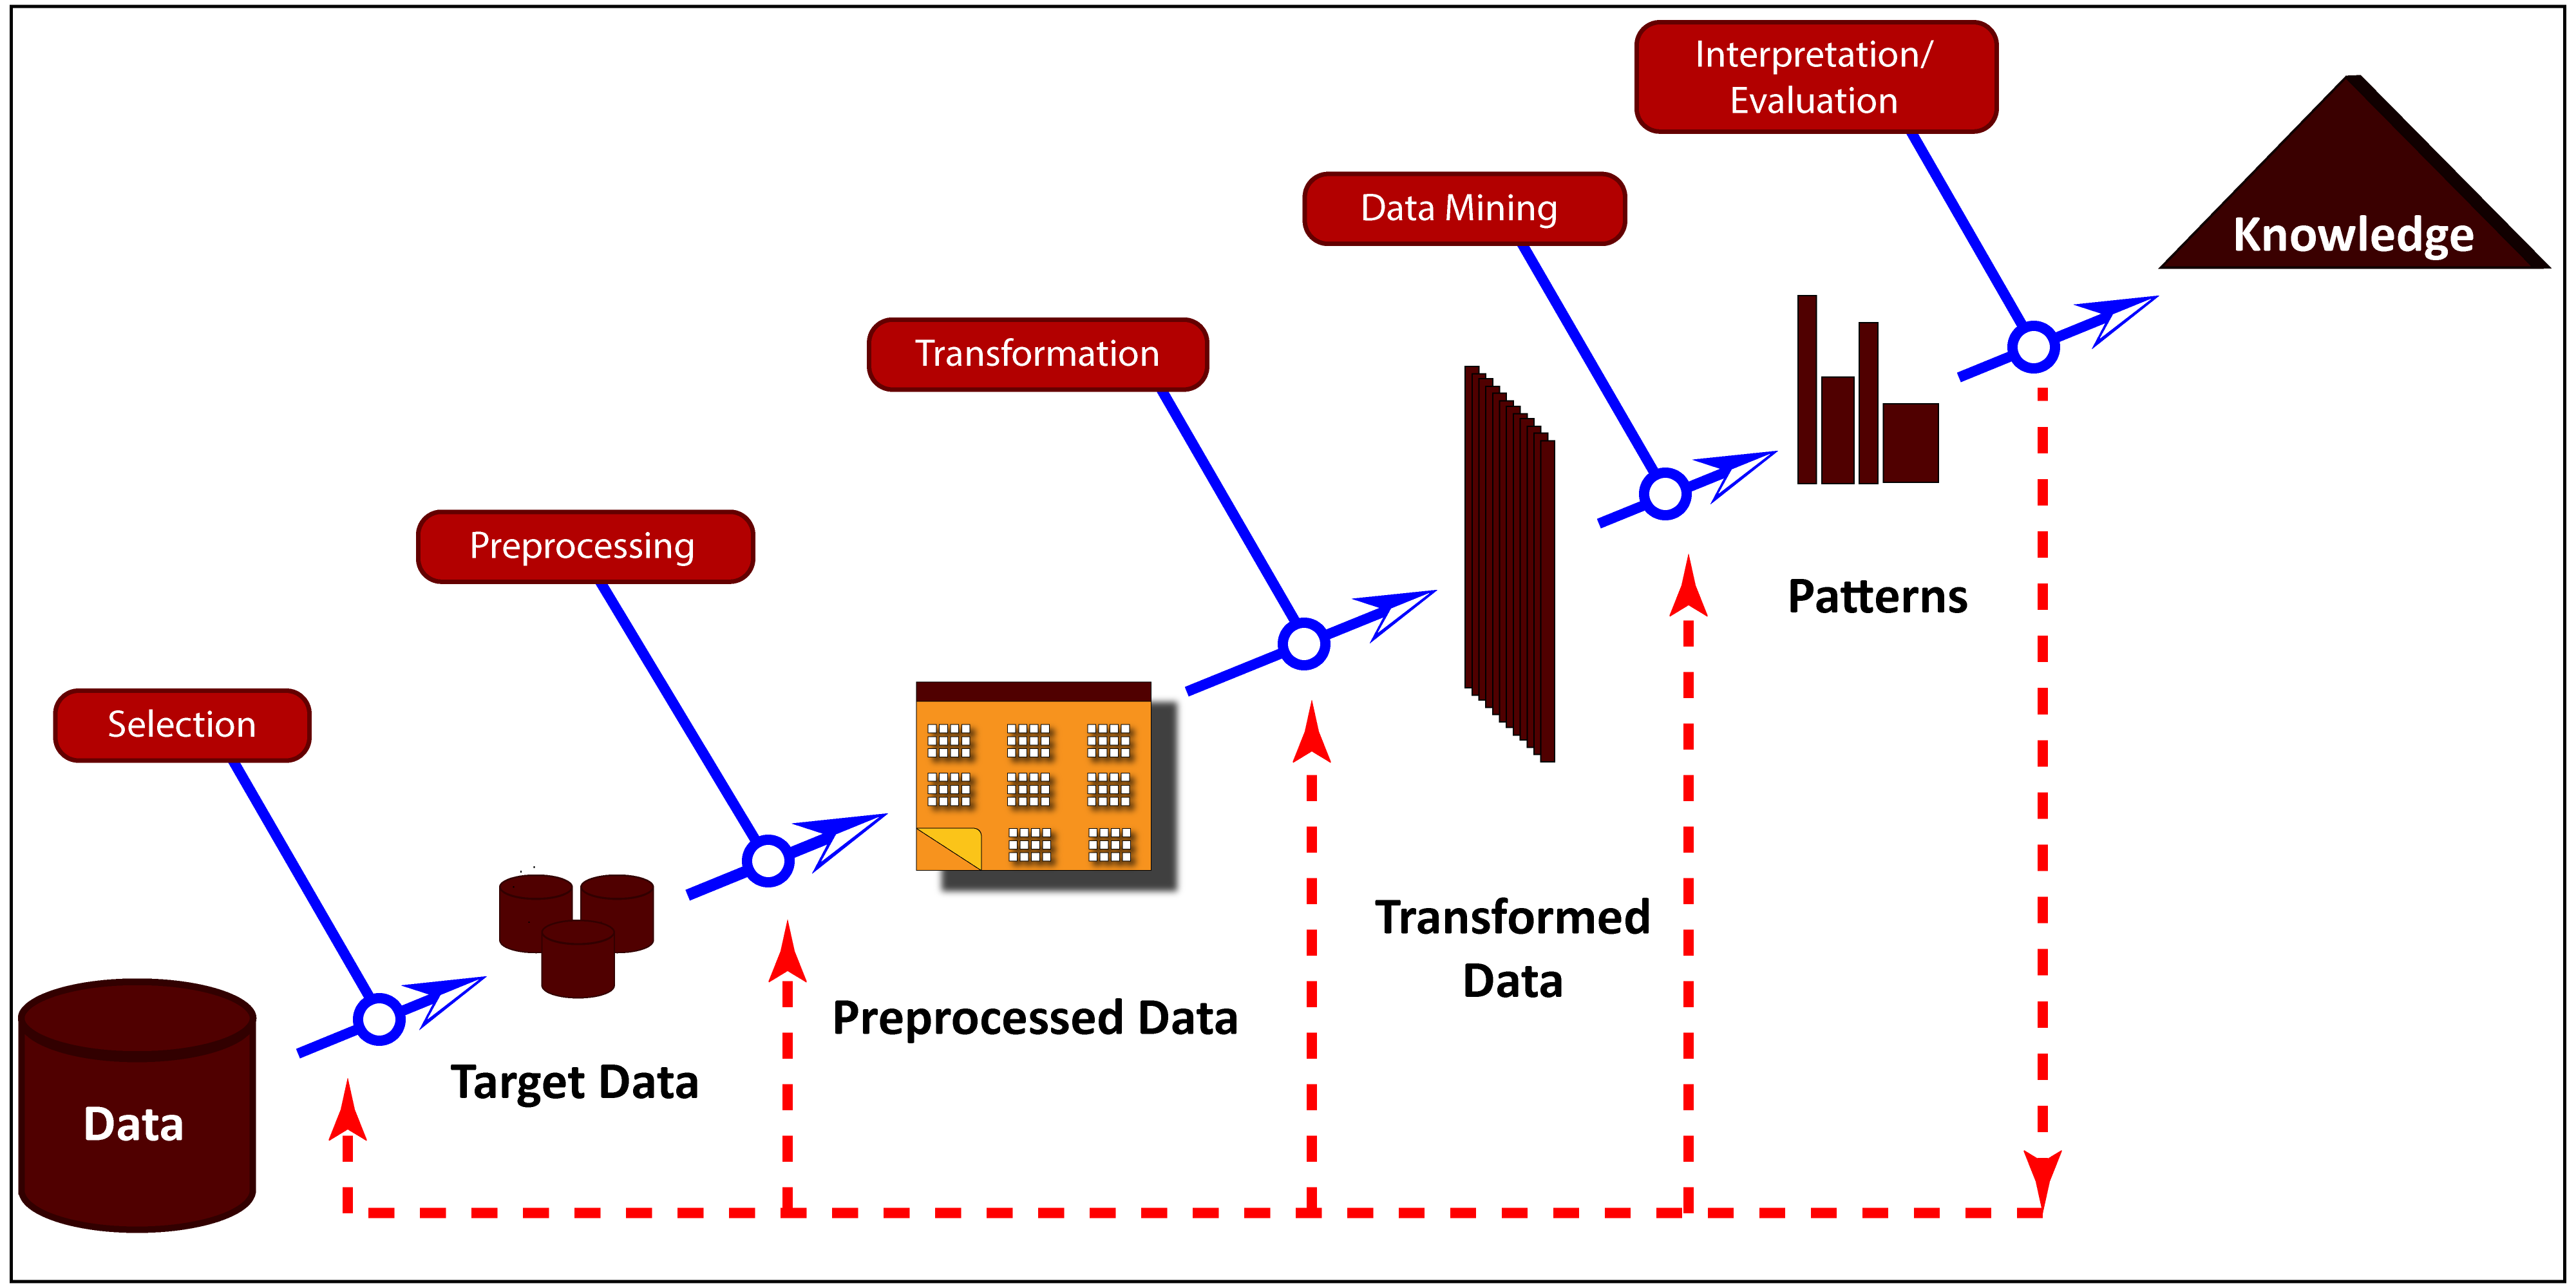
\includegraphics[width=\textwidth]{images/chapitre1/extract_data_steps.png}
		\end{center}
    \caption{Les étapes de l'extraction de connaissances à partir de données}
    \label{extraction_connaissances}
    \end{figure}
    
    \subsection{Les méthodes du data mining}
    Le clustering et la classification sont deux tâches fondamentales dans l'exploration de données.
    La classification est principalement utilisée comme méthode d'apprentissage supervisé, le clustering pour 
    l'apprentissage non supervisé (certains modèles de clustering sont pour les deux). Le but du clustering est descriptif, 
    celui de la classification est prédictif (Veyssieres et Plant, 1998). \\
    « Comprendre notre monde nécessite de conceptualiser les similitudes et les différences entre les entités qui 
    le composent » (Tyron et Bailey, 1970) \cite{Educational_data_mining_a_survey_from_1995_to_2005}. De ce fait, certains coefficients de corrélations sont utilisés pour 
    calculer la similarité entre deux éléments ou plusieurs et, des métriques et les critères de liaison permettent 
    qu’en ta eux de déterminer le lien entre plusieurs entités afin de les groupées dans une même classe 
    (c’est le cas du clustering). \\
    Certaines méthodes comme : rule of association, preaching, neural networks, decision trees sont utilisé aussi pour 
    explorer et analyser des jeux de données.

    \section{Intelligent Tutorial Systems (ITS)}

    \subsection{Définition}
    Les systèmes de tutorat intelligents (ITS) sont des environnements d'apprentissage informatisés issus de l'IALT 
    (Intelligent Computer Assisted Instruction) qui visent à personnaliser la formation. En effet, ils ont été développés 
    pour répondre aux limites du CAI (Computer Assisted Instruction) en utilisant l'intelligence artificielle pour mettre 
    en œuvre des systèmes plus flexibles et interactifs qui s'adaptent « aux besoins spécifiques de l'apprenant en évaluant 
    et en diagnostiquant ses problèmes afin de fournir les assistances » (Buche C., 2005). L'objectif est de mimer le 
    comportement d'un tuteur humain en sa qualité de pédagogue expert et d'expert dans le domaine. Ainsi, tout comme 
    un tuteur, un logiciel de ce type a le potentiel d'amener l'apprenant à accomplir une tâche et à fournir un retour 
    sur leurs actions. ITS répond ainsi à la nécessité de placer l'apprenant au centre du processus d'apprentissage \cite{buche:tel-00011223}. \\
    Les ITS sont essentiellement un environnement de résolution de problèmes ou d'exercice. Ils favorisent l'apprentissage 
    dans un domaine spécifique en guidant et en aidant l'apprenant. Parfois, ils exposent d'abord le contenu de la matière 
    à l’apprenant ; parfois ils présentent directement les exercices qui permettront à l'apprenant d'assimiler les 
    connaissances \cite{handbook_of_educational_data_mining}.

    \begin{figure}[H]
		\begin{center}
			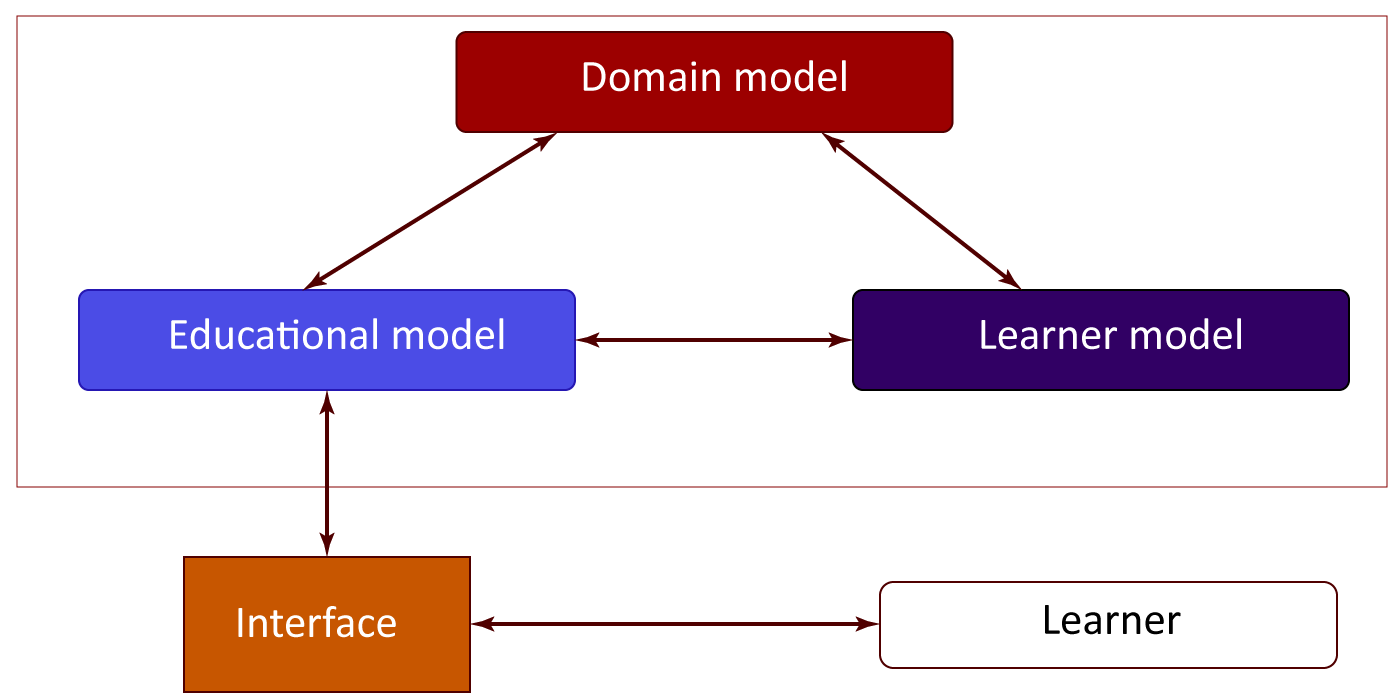
\includegraphics[width=\textwidth]{images/chapitre1/ITS architecture}
		\end{center}
    \caption{ITS architecture}
    \label{itsArchitecture}
    \end{figure}

    \subsection{ITS architecture}
    L'architecture conceptuelle d'un ITS est illustrée à la figure \ref{itsArchitecture} et comprend : \cite{handbook_of_educational_data_mining}
    \begin{itemize}
		    \item[$\bullet$] \textbf{Un modèle de l'interface :} qui représente la couche de communication entre l'apprenant et le système, c'est-à-dire les interactions entre l'apprenant et le système. Cette interface peut faire varier le type d'environnement d'apprentissage et l'objectif étant de privilégier une approche de conception qui ne gêne pas l'apprentissage. La qualité de l'interaction peut influencer les résultats d'apprentissage. Par conséquent, les principaux problèmes avec les interfaces d'apprentissage sont les problèmes d'interaction personne / machine. Pour surmonter ces problèmes, il faut prêter attention à la convivialité pour que la charge mentale associée à l’interface soit négligeable, ainsi qu’à l’utilité en facilitant l’accès, en permettant l’accès au domaine d’apprentissage et en soutenant la métacognition de l’apprenant. Les tendances actuelles s'orientent vers des dialogues tutoriels en langage naturel, l'intégration de la dimension affective dans l'interaction et les interfaces tangibles.
		
		    \item[$\bullet$] \textbf{Modèle du domaine :} également appelé modèle expert, il représente l'expertise de l'enseignant dans le domaine, c'est-à-dire ce qui doit être enseigné. Elle peut être modélisée de trois manières : une approche « boîte noire » : appliquer toute méthode de raisonnement sur le domaine inexpliqué, sans aucune transparence pour l'utilisateur ; un système expert peut expliquer son raisonnement et un modèle cognitif : simuler la manière dont les humains utilisent les connaissances.
        
        \item[$\bullet$] \textbf{Un modèle d'apprentissage :} qui peut personnaliser l'apprentissage en tenant compte des spécificités de l'apprenant.
        
        \item[$\bullet$] \textbf{Un modèle éducatif :} qui sait enseigner.

    \end{itemize}
    
    \section{Educational Data mining}
    \subsection{Définition}
    La communauté d'exploration de données appliquée dans l'éducation a défini ce terme comme suit : 
    « L'exploration de données appliquée dans l'éducation est une discipline qui concerne le développement de méthodes
     permettant d'explorer les types uniques de données provenant des milieux éducatifs. Ces méthodes sont utilisées 
     pour mieux comprendre le comportement des apprenants et environnement de leur apprentissage. » \cite{state_of_educational_data_mining_in_2009_a_review_and_future_visions} \\
    L'exploration de données éducatives (EDM) vise à développer, rechercher et appliquer des méthodes informatisées
     pour détecter des modèles dans de grandes collections de données éducatives qui seraient autrement difficiles 
     ou impossibles à analyser en raison de l'énorme volume de données dans lesquelles elles existent \cite{Educational_data_mining_a_survey_from_1995_to_2005}. \\
    Ce domaine est une forme d'intersection des trois domaines principaux tels que : l'informatique, l'éducation 
    et les statistiques illustrés dans la figure \ref{domaine_exploration_données}.

    \begin{figure}[H]
		\begin{center}
			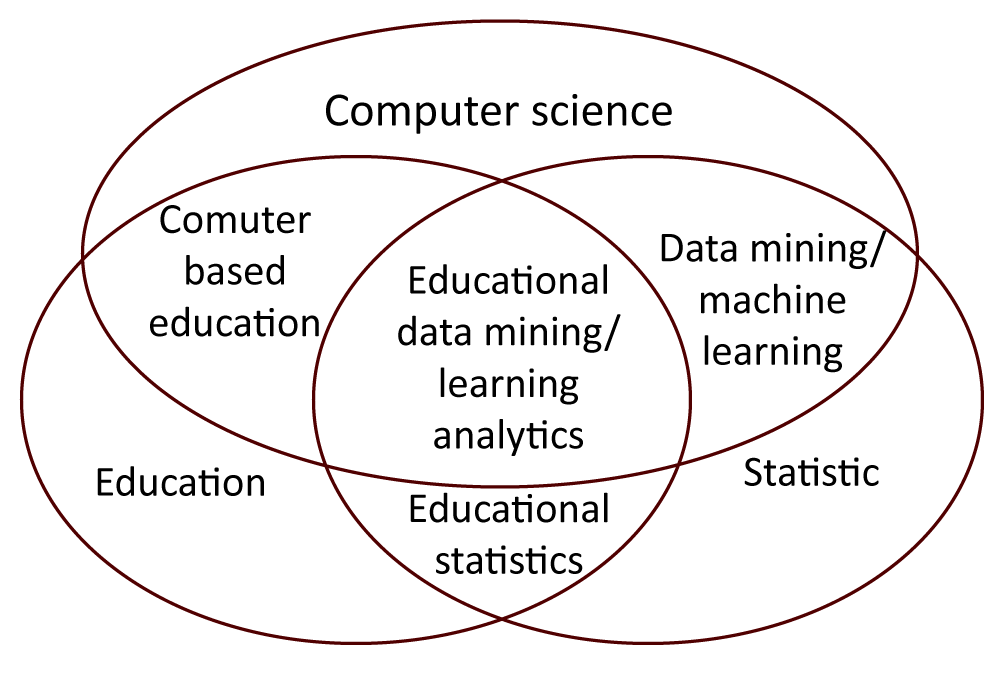
\includegraphics[width=\textwidth]{images/chapitre1/Principaux domaines liés à l'exploration de données éducatives}
		\end{center}
    \caption{Principaux domaines liés à l'exploration de données éducatives}
    \label{domaine_exploration_données}
    \end{figure}

    Les techniques d'exploration de données (EDM) sont devenues plus importantes dans la recherche et le développement en raison du développement rapide de la technologie, de la croissance rapide des connaissances humaines et de l'augmentation du nombre de personnes détenant des systèmes d'enseignement informatisé. \\
    
    \subsection{Processus d'application du DM en éducation}
    Le processus d'application de l'exploration de données appliqué dans l'éducation peut être considéré comme
    un cycle itératif de formulation, de test et de raffinement d'hypothèses. Dans ce processus, l'objectif n'est pas seulement de transformer les données en connaissances, mais aussi de filtrer les connaissances extraites pour savoir comment les modifier. \\
    L’environnement éducatif pour améliorer l’apprentissage des apprenants est présenté dans la figure \ref{dataMiningProcess}. Des études ont montré que l'application de l'EDM est similaire au processus Knowledge from Data (KDD). Ce processus commence par la collecte de données à utiliser à partir de l'environnement éducatif. \\
    Les données brutes obtenues nécessitent un nettoyage et un prétraitement tels que : fusion de données hétérogènes, traitement des données manquantes, conversion de données d'une source de données à une autre, et données, etc. Cette phase nécessite souvent l'utilisation de certaines données techniques minières. \\
    Le résultat de ce dernier est un modèle capable de structurer les données stockées. Enfin, la dernière étape est l'interprétation et l'évaluation des résultats obtenus \cite{dm_tuteurs}.

    \begin{figure}[H]
		\begin{center}
			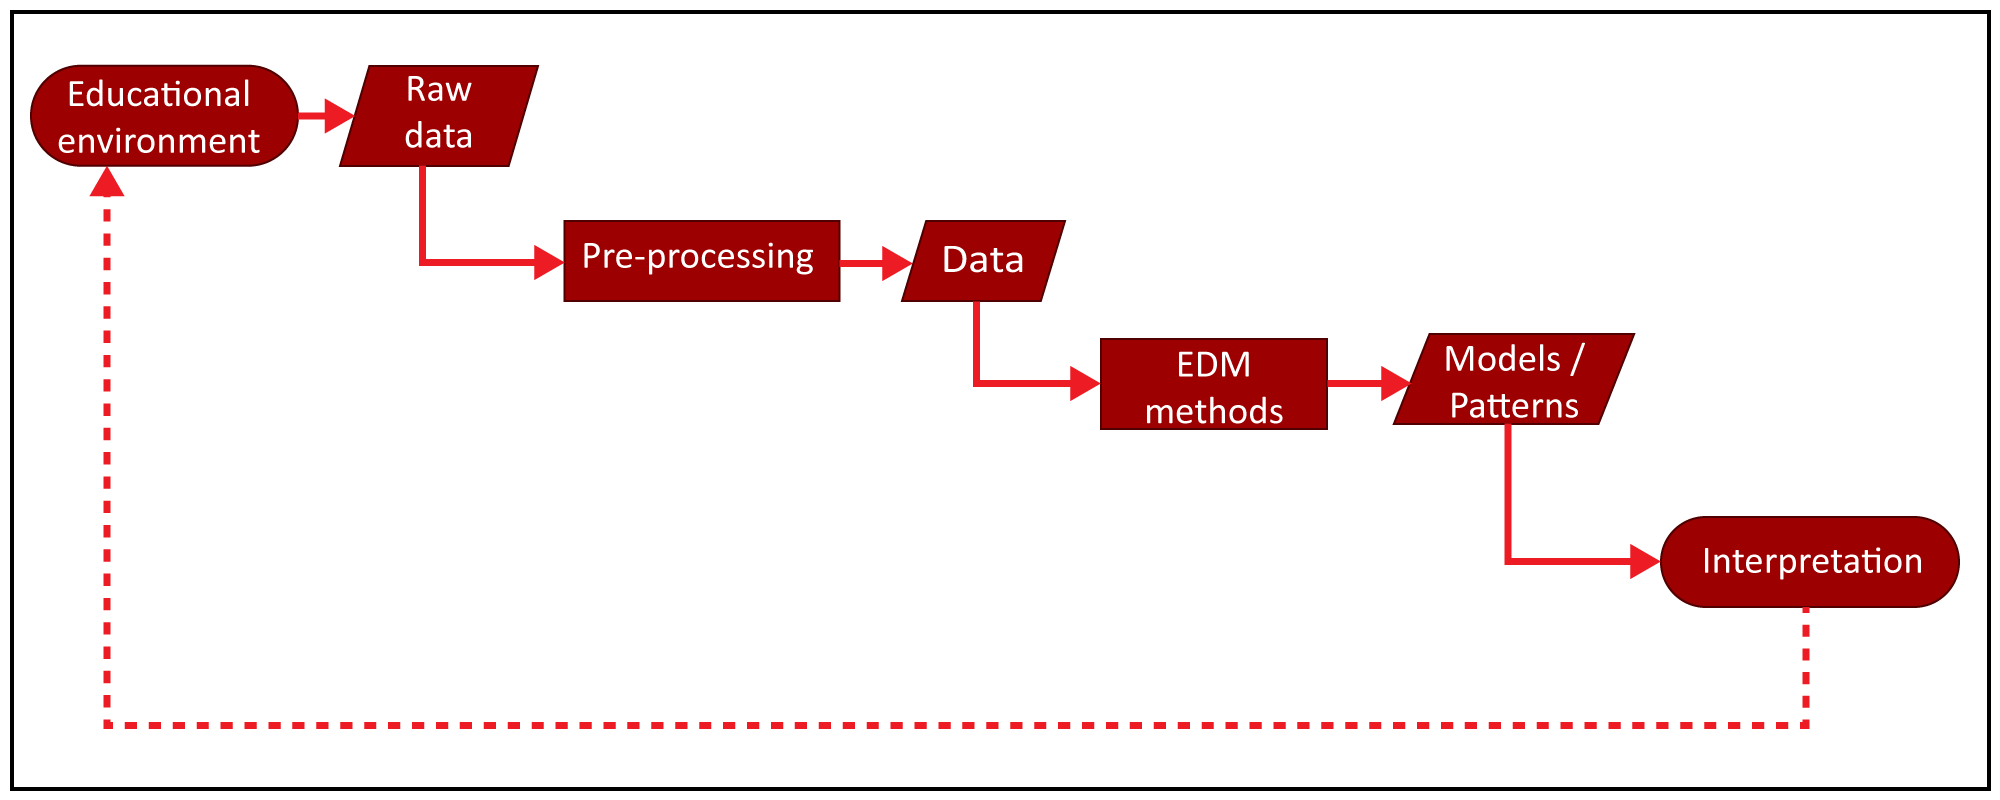
\includegraphics[width=\textwidth]{images/chapitre1/Data mining application process applied in education}
		\end{center}
    \caption{Data mining application process applied in education}
    \label{dataMiningProcess}
    \end{figure}

    \subsubsection{Les méthodes d’analyse et d’exploration appliquer dans EDM}
    Certaines méthodes du data mining ont été largement appliquées sur les données issues des systèmes éducatif 
    afin d’obtenir des connaissances cacher et des modèles. Les méthodes du data mining ont été appliquer dans 
    plusieurs domaines de recherche tels que : le e-learning, le système de tuteur intelligent, text mining, 
    réseaux sociaux, web mining, etc. Les méthodes d’analyse et d'exploration de données éducatives sont 
    tirées de diverses sources littéraires, notamment l'apprentissage automatique, la psychométrie et d'autres 
    domaines de la modélisation informatique, des statistiques et de la visualisation de l'information. \\

    \begin{figure}[H]
		\begin{center}
			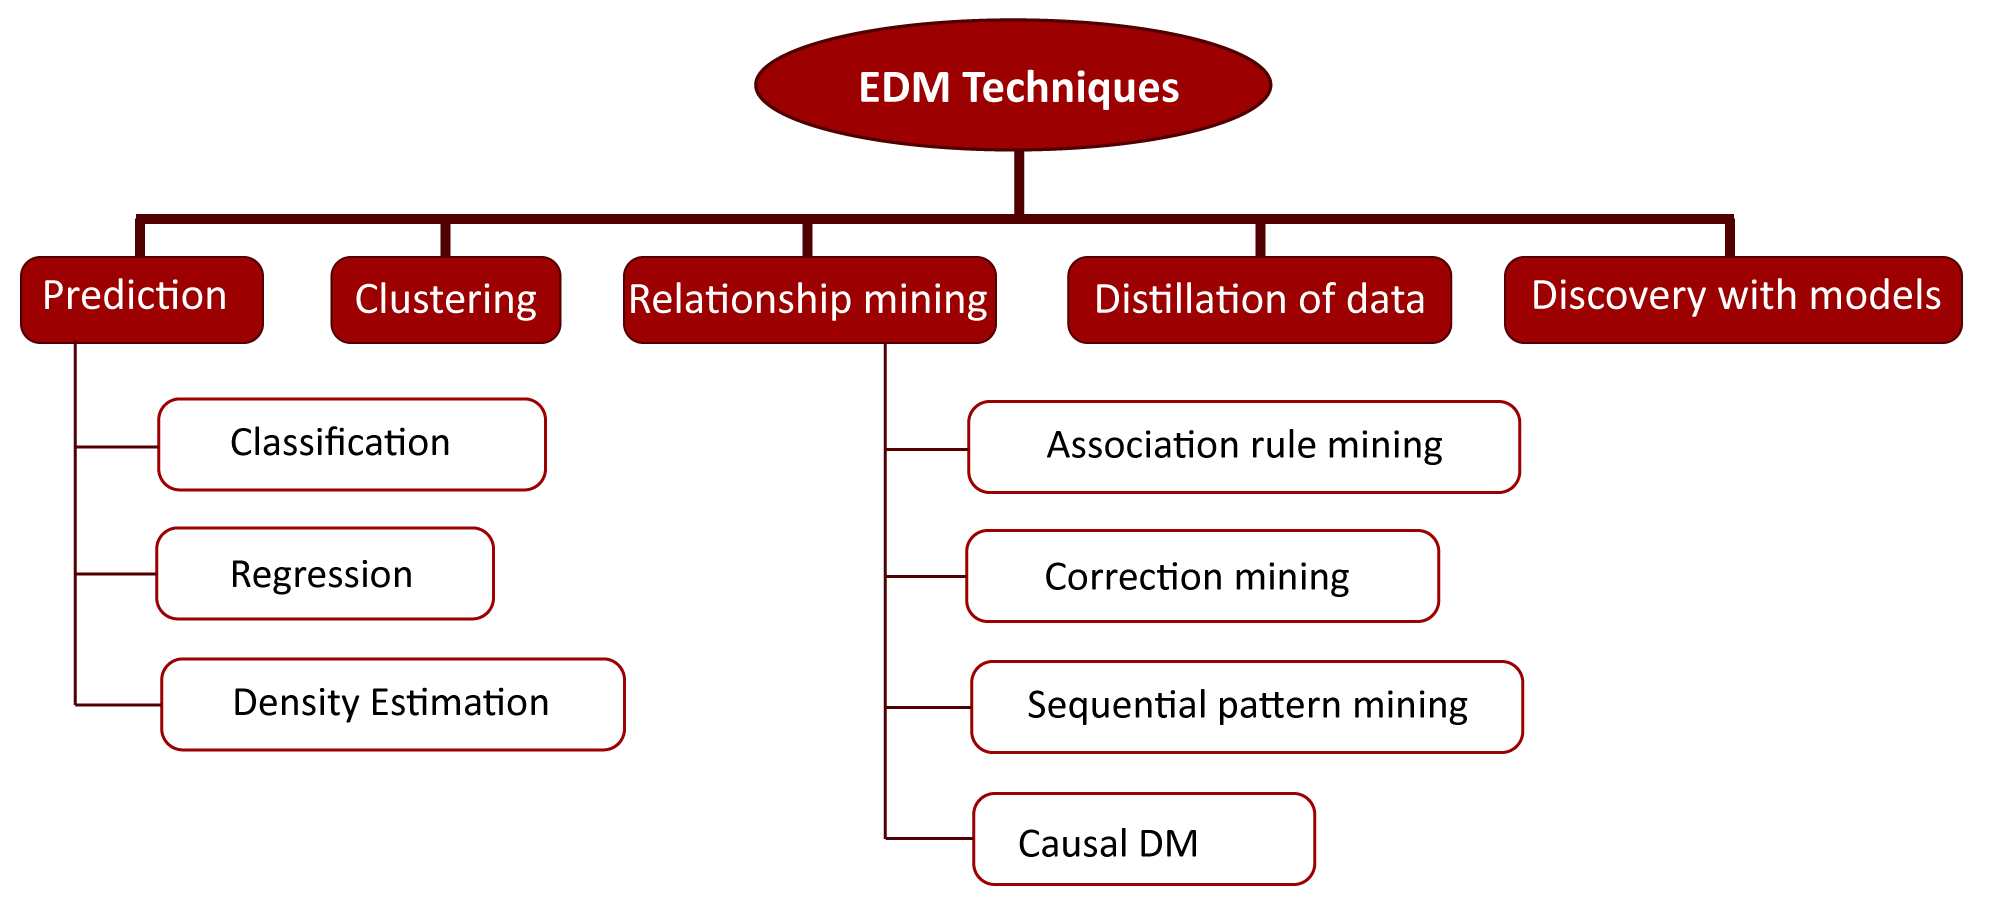
\includegraphics[width=\textwidth]{images/chapitre1/edm techniques}
		\end{center}
		\caption{EDM techniques}
    \end{figure}

    \paragraph{L'induction de modèle supervisée}

    L'induction de modèle supervisée comprend des techniques d'apprentissage automatique qui déduisent des modèles de prédiction à partir de instances d'entraînement pour lesquelles les valeurs d'un attribut cible sont connues. Les modèles de prédiction acceptent
    instances en entrée (généralement décrites comme un vecteur d'attribut) et en sortie une prédiction pour la cible attribut. Les modèles qui prédisent des valeurs cibles catégorielles sont appelés modèles de classification ; des modèles qui prédire les valeurs cibles continues sont appelés modèles de régression. Les modèles de prédiction peuvent être basés sur
    différentes représentations, par exemple, les arbres de décision, les machines à vecteurs de support (les deux classifications) et modèle de régression linéaire (régression) \cite{Scheuer2012}.

    \paragraph{L'induction de modèle non supervisée}

    L'induction de modèle non supervisée comprend des techniques d'apprentissage automatique qui déduisent des modèles à partir d'instances d'apprentissage pour lesquelles les valeurs d'un attribut cible ne sont pas connues. 
    Les méthodes non supervisées utilisent une approche ascendante, c'est-à-dire que les modèles et les structures 
    sont recherchés dans l'espace d'entrée sans catégories cibles explicitement définies ni exemples étiquetés. 
    Une approche largement utilisée est le clustering, qui est utilisé pour identifier des groupes d'instances dans 
    un ensemble d'apprentissage qui sont « similaires » à certains égards. En règle générale, une sorte de mesure de 
    distance (par exemple, la distance euclidienne) est utilisée pour décider de la similitude des instances. Une fois un 
    ensemble de clusters a été déterminé, de nouvelles instances peuvent être classées en déterminant le cluster le plus 
    proche. Un algorithme de clustering bien connu est le clustering k-means \cite{Scheuer2012}.
    
    \paragraph{L'estimation des paramètres}
    L'estimation des paramètres comprend des techniques statistiques pour déduire des paramètres de modèles probabilistes à partir d’un jeu de données. Ces modèles peuvent être utilisés pour prédire la probabilité d'événements d'intérêt. L'approche est basée sur l'hypothèse que le modèle a une forme paramétrique donnée (par exemple, une distribution gaussienne avec les paramètres moyenne et variance). Un exemple d'application en EDM est l'estimation des paramètres Bayesian Knowledge Tracing (BKT). Le BKT est utilisé pour déterminer la probabilité qu'un élève maîtrise une compétence sur la base de l'historique des performances passées. Un modèle BKT peut être compris comme un réseau bayésien dynamique avec quatre paramètres (priorité, estimation, glissement et taux d'apprentissage). Ces paramètres peuvent être déterminés, par exemple, avec l'algorithme Espérance-Maximisation. Aussi l’utilisation de la théorie des réponses aux items (Item Response Theory IRT) permet de capter plus de nuances dans le comportement humais et d’estimer la capacité de l’apprenant à réussir un item et aussi d’estimer la difficulté, la discrimination des items \cite{Scheuer2012}.

    \paragraph{L'exploration de relations (Relationship mining)}
    L'exploration de relations concerne l'identification des relations entre les variables, des relations qui peuvent être de nature associative, corrélationnelle, séquentielle ou causale. Par exemple, une approche courante de l'exploration de règles d'association consiste à apprendre les règles SI-ALORS qui dépassent un seuil minimum de « support » et de « confiance ». La prise en charge indique la fréquence relative des transactions qui correspondent à la fois aux parties IF et ALORS de la règle. La confiance dénote la fréquence relative des transactions qui correspondent à la partie THEN de la règle dans l'ensemble de transactions qui correspondent à la partie IF. Apriori est, par exemple, un algorithme de règle d'association classique. Un exemple d'application en EDM est l'identification d'erreurs qui se produisent fréquemment ensemble (par exemple, les étudiants qui ont commis les erreurs A et B ont également souvent commis l'erreur C) \cite{Scheuer2012}.
    
    \paragraph{La distillation des données pour le jugement humain (Distillation of data for human judgment)}
    La distillation des données pour le jugement humain vise à représenter les données de manière intelligible à l'aide de statistiques, méthodes de visualisation et interfaces d'information interactives. Par exemple, les performances moyennes les scores peuvent être calculés pour chaque élève et présentés à un enseignant par ordre croissant dans un graphique à barres. Un autre exemple est les courbes d'apprentissage, qui tracent les performances d'un élève (par exemple, le temps de réponse) par rapport au nombre d'occasions de pratiquer une compétence. Une courbe d'apprentissage idéale montre que la performance s'améliore en douceur et de façon monotone, suivant approximativement une loi de puissance ou une fonction exponentielle. D'un autre côté, les courbes d'apprentissage avec des pointes indiquent qu'une autre compétence pourrait interférer avec la compétence réellement modélisée, c'est-à-dire que le modèle de compétence pourrait être amélioré \cite{Scheuer2012}.
    
    \paragraph{Discovery with models}
    Discovery with models (découverte avec des modèles) comprend des approches qui amorcent des modèles déjà existants pour faire des découvertes plutôt que de calculer de nouveaux modèles à partir de zéro. Par exemple, un modèle de prédiction pourrait être appliqué à un ensemble de données pour prédire les valeurs d'une catégorie cible d'intérêt. Les prédictions elles-mêmes pourraient être utilisés à nouveau comme données dans d'autres analyses, par exemple, ils pourraient être corrélés avec une catégorie cible d’un autre modèle de prédiction. Un autre exemple consiste à scruter les différentes composantes d'un modèle de prédiction pour en savoir plus sur les facteurs qui influencent la prédiction \cite{Scheuer2012}.
    
    \section{Conclusion}
    Dans ce chapitre, nous avons passé en revue le domaine de l'exploration de données éducatives, en présentant brièvement ses applications et ses techniques. L'application des méthodes d'exploration de données dans le secteur de l'éducation est un phénomène intéressant. Les techniques d'exploration de données dans les organisations éducatives nous aident à en apprendre davantage sur les performances des apprenants, le comportement des apprenants, la conception des programmes et à motiver les apprenants sur divers paramètres.
	
	
\chapter{Modèle de l'apprenant et découverte des prérequis} 
\minitoc
\thispagestyle{empty}
\newpage
\section{Introduction}
Le terme "apprentissage" fait souvent référence à l'apprentissage électronique ou e-learning. L’apprentissage en ligne, l'apprentissage à distance et l'apprentissage en ligne. L'apprentissage en ligne est connu comme des activités d'étude avec le soutien d'un ordinateur et d'un réseau (Fröschl, 2005, p. 12). \\
Dans l'apprentissage en ligne, la communication entre les apprenants et les enseignants ou les apprenants et les apprenants se fait sur le réseau ou sur Internet, les supports d'apprentissage sont souvent des documents électroniques tels que des pages Web et des fichiers au lieu de livres traditionnels sur papier \cite{learner_model__adaptive_learning}. Dans ce chapitre, nous décrivons la modélisation de l'apprenant compte tenu de son importance dans tous les domaines de recherche. Nous commençons par une présentation des notions du modèle de l'apprenant et des caractéristiques des méthodes utilisées pour la modélisation de l'apprenant. Puis nous terminons avec la Découverte des prérequis.

\section{Learner Model}

\subsection{Définition}
Winkels décrit le modèle de l'apprenant comme une structure de données qui reflète l'état des connaissances supposées de l'apprenant sur un domaine cible (le domaine d'apprentissage) \cite{user_modelling_help_systems}. Selon Self, le modèle de l'apprenant devrait inclure les informations suivantes : les connaissances et les idées fausses de l'apprenant, ses compétences et son comportement. Pour déterminer ce que l’apprenant a fait, Self souligne qu’il est nécessaire d’avoir un historique des interactions de l’apprenant avec le système \cite{user_learner_modeling_workbench}. \\
Greer considère le modèle de l'apprenant comme une représentation abstraite des croyances, des connaissances et des compétences de l'apprenant dans le système, y compris l'historique des actions de l'apprenant qui peut être analysé et interprété \cite{psycho_oncology}.

\subsubsection{Caractéristiques des méthodes utilisées pour la modélisation de l'apprenant}
Il existe plusieurs modèles existants classés selon la nature des informations extraites par le modèle et les méthodes utilisées pour les traiter \ref{Caracteristiques_modelisation_apprenants1}\ref{Caracteristiques_modelisation_apprenants2}.[5]

\begin{table}[!htbp]
	\begin{tabular}{|m{3cm}|m{4cm}|m{4cm}|m{4cm}|} %\rule{0pt}{1.5\normalbaselineskip}
	\hline
	\rowcolor{blueforest}
	\color{white} \textbf{Méthodes} & \color{white} \textbf{Applications} & \color{white} \textbf{Avantage} & \color{white} \textbf{Limites} \\
	\hline\hline
	\textbf{Modèle de superposition} \newline {------------------} \newline  \textbf{Modèle différentiel}   &
	  Modélisation des connaissances  de l'apprenant à travers   le modèle de connaissance. \newline {-------------------------------} \newline  Identification des lacunes dans les connaissances des apprenants &
	  -Haute expressivité des   problèmes complexes et   flexibilité du raisonnement humain.\newline - utilisation de la structure   du modèle de connaissance.&
	  -Impossible de détecter   les erreurs de l'apprenant \newline -La complexité dépend de   la structure du domaine. \newline  - Défaut de modéliser   les erreurs de l'apprenant. \\ \hline
	  \textbf{Modèle d'erreur}  &
	  Identification des erreurs et fausses croyances de l'apprenant sur un domaine.&
	  Identification des erreurs et fausses croyances de l'apprenant dans un domaine.&
	  Difficulté à modéliser et à définir les erreurs. \\ \hline
	  \textbf{Stéréotypes}  &
	  Classification des apprenants selon des caractéristiques communes, les plus utilisées sont : le style d'apprentissage, le style cognitif, le niveau de connaissance et les préférences.&
	  Initialisation de nouveau caractéristiques de l'apprenant. & \\ \hline
	  \textbf{Les ontologies}  &
	  -Modélisation du modèle de connaissance. \newline
	  -Réutilisation et partage des ressources.&
	  -Ajout de sémantique aux relations entre concepts. \newline
	  -Réutilisation des ressources.&  \\ \hline
	  \textbf{Logique floue}  &
	  -Expression linguistique du niveau de connaissance. \newline
	  -Évaluation des apprenants.\newline
	  -Identification du style de l'apprenant.&
	  -Expression du degré d'incertitude. \newline
	  -Grande expressivité linguistique et logique.&
	  -Consommation de ressources \newline
	  -Pas d'apprentissage. \\ \hline
	\end{tabular}
	\caption{Caractéristiques des méthodes utilisées pour la modélisation des apprenants partie[1]}
	\label{Caracteristiques_modelisation_apprenants1}
\end{table}

\begin{table}[!htbp]
	\begin{tabular}{|m{3cm}|m{4cm}|m{4cm}|m{4cm}|} %\rule{0pt}{1.5\normalbaselineskip}
	\hline
	\rowcolor{blueforest}
	\color{white} \textbf{Méthodes} & \color{white} \textbf{Applications} & \color{white} \textbf{Avantage} & \color{white} \textbf{Limites} \\
	\hline\hline
	  \textbf{Réseau Bayésien}  &
	  -Apprendre et prédire le comportement et le raisonnement de l'apprenant. \newline
	  -Classement des apprenants. \newline
	  -Prédiction des performances des apprenants.&
	  -Apprendre et s'adapter à un environnement incertain.\newline
	  -Résoudre le problème « onlearning » \newline
	  -Fonction avec des données manquantes.&
	  -Consommation de ressources \newline
	  -Difficulté à comprendre les inférences (interprétation) \newline
	  -Grand nombre de variables utilisées. \\ \hline
	  \textbf{Programmation génétique}  &
	  - Recommandation d'un chemin de navigation optimal. \newline
	  -Prédiction des performances des apprenants. \newline
	  -Amélioration des algorithmes de classification.&
	  -Recherche globale \newline
	  -représentation flexible aux changements. \newline
	  -des recherches puissantes dans un espace de problèmes complexes et mal définis.&
	  -Temps d'exécution \newline
	  -Convergence vers les optima locaux \\ \hline
	  \textbf{Réseau flou de neurones}  &
	  -Évaluation et prédiction des performances des apprenants.&
	  -Grand Expressivement \newline
	  -Apprentissage \newline
	  -gestion des incertitudes.&
	  La complexité augmente avec le nombre d'entrées du réseau. \\ \hline
	\end{tabular}
	\caption{Caractéristiques des méthodes utilisées pour la modélisation des apprenants partie[2]}
	\label{Caracteristiques_modelisation_apprenants2}
\end{table}

\subsection{Composantes du modèle de l'apprenant}
\begin{figure}[H]
	\begin{center}
		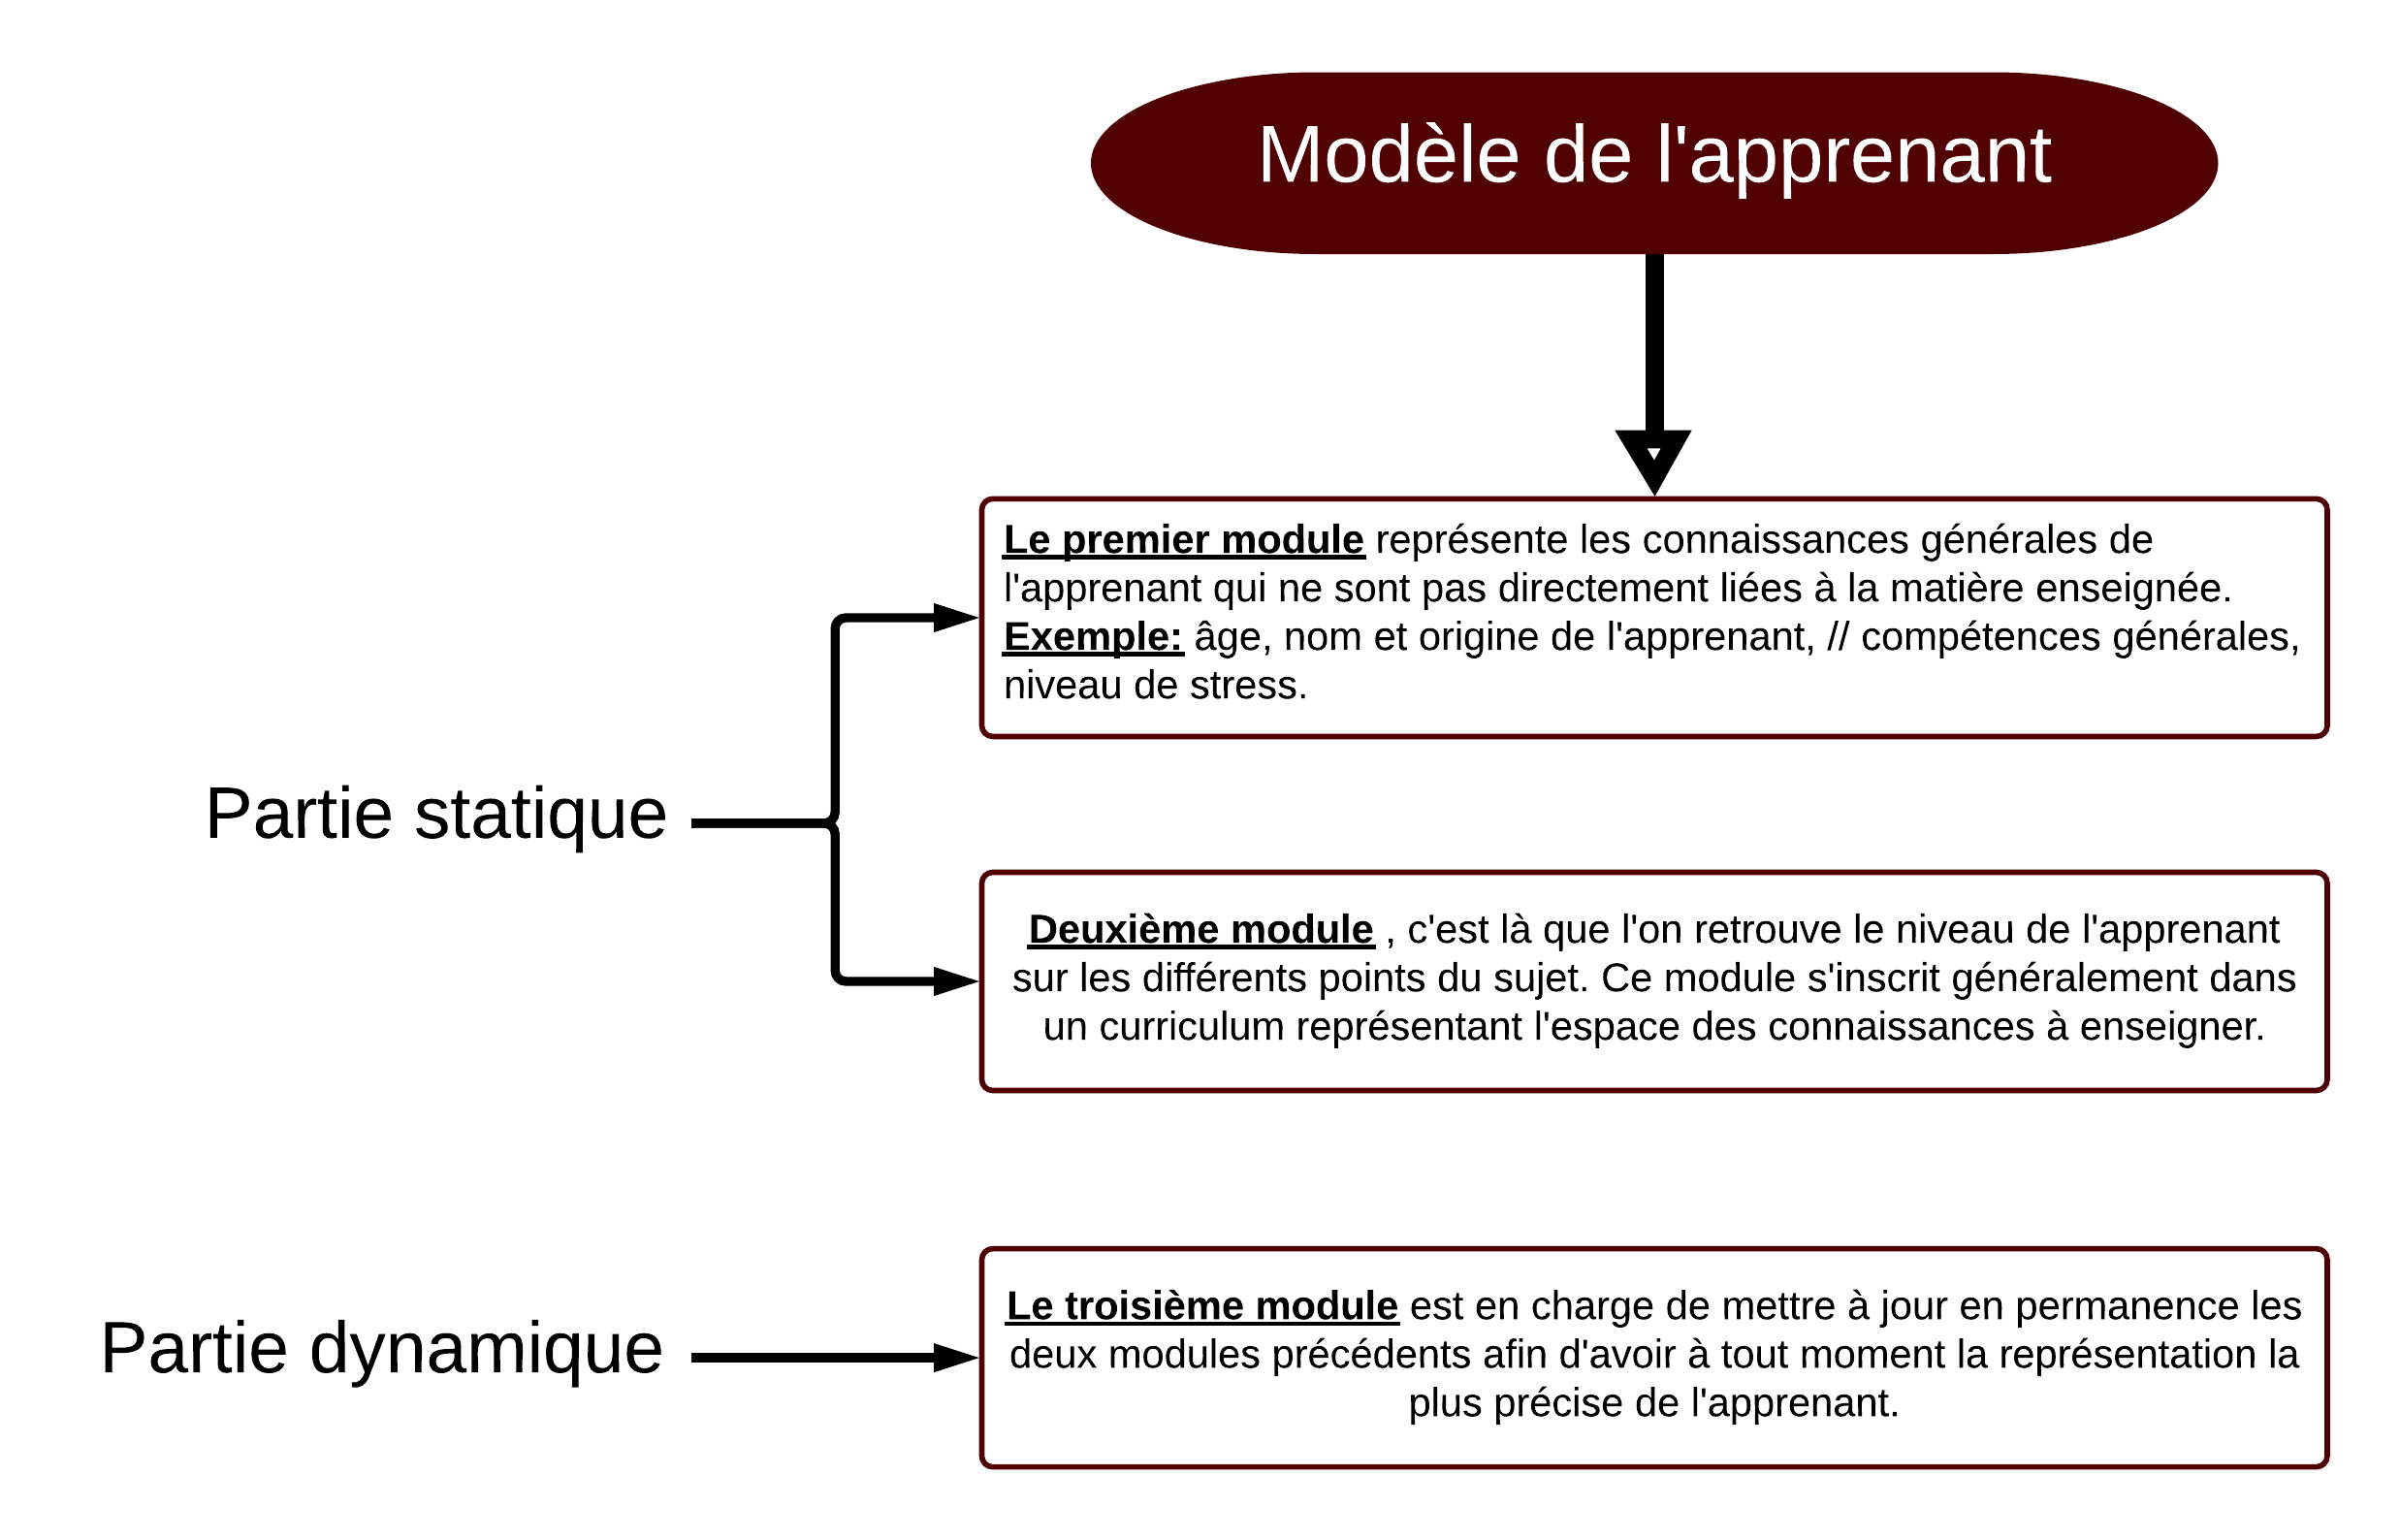
\includegraphics[width=\textwidth]{images/chapitre2/Learner_model.png}
	\end{center}
\caption{Composantes du modèle de l'apprenant}
\label{learnerModel}
\end{figure}
Carr et Goldstein citent, par exemple, quatre informations nécessaires pour maintenir ce modèle : la difficulté du sujet, les questions directement posées par l’apprenant, la performance de l’apprenant et son expérience d’apprentissage. [6] Self définit le modèle de l'apprenant comme un 4-tuplet contenant les variables P (connaissance procédurale), C (connaissance conceptuelle), T (caractéristiques individuelles) et H (histoire). [7] \\
Un modèle de l'apprenant \ref{learnerModel} comprend toujours des connaissances liées au domaine d'enseignement : ce que l'apprenant sait et ce que l'apprenant peut faire. Dans son état le plus complet, ce modèle comprend également des connaissances indépendantes du domaine enseigné. Certaines de ces connaissances sont liées à ses mécanismes d'apprentissage : comment fonctionne l'apprenant ? Comment découvre-t-il de nouveaux concepts ? De nouvelles techniques ? Etc. Les autres concernent les stratégies pédagogiques correspondantes : quels sont les types et modalités d'intervention les plus efficaces ? Etc. \\
Selon Nkambou, le modèle de l'apprenant est identifié en trois parties: [8]

\subsubsection{Modèle cognitif}
Description de l’état des connaissances de l’apprenant par rapport au sujet considéré par le bailleur de fonds. Ces informations concernent :
\begin{itemize}
	\item[$\bullet$] Capacités : les informations sur les capacités reflètent le niveau de connaissances de l'apprenant. Robert M. Gagne a classé les capacités de l’apprenant en cinq catégories : l’information verbale, les compétences intellectuelles, les attitudes, la motricité et les stratégies cognitives.
	\item[$\bullet$] Objectifs : les informations sur les objectifs indiquent si l'apprenant a déjà atteint ou non un objectif.
	\item[$\bullet$] Ressources : les informations sur les ressources (exercices, problèmes, tests, etc.) reflètent le fait qu'une ressource a déjà été utilisée par un apprenant et le contexte dans lequel cette ressource a été utilisée.
	\item[$\bullet$] Relations éventuelles : les informations sur les relations indiquent si l'apprenant a réussi ou échoué à établir une relation (par exemple, analogie, abstraction, cas particulier, etc.) entre deux connaissances (et par conséquent, la connaissance d'une relation entre deux connaissances est aussi connaissance (méta-connaissance)).
\end{itemize}

\subsubsection{Modèle d'inférence}
Cette partie est une sorte de moteur d’inférence qui fonctionne en permanence pour ajuster le modèle de l’apprenant. Il contient des règles qui lui permettent de raisonner sur le modèle cognitif et sur le modèle psychologique (modèle affectif) pour inférer de nouvelles connaissances dans le modèle de l’apprenant.

\subsubsection{Modèle émotionnel}
Ce modèle est un ensemble de données qui nous permet d'identifier la personnalité et les différentes facettes d'un apprenant. Il contient des connaissances sur les caractéristiques permanentes ou momentanées particulières de l’apprenant. Parmi ceux-ci, nous avons :
\begin{itemize}
	\item[$\bullet$] Connaissance des conditions mentales PUX. Par exemple, l'apprenant est spatial ou verbal, réfléchi ou impulsif, etc.
	\item[$\bullet$] Connaissance des sentiments et de la personnalité. Par exemple, l'apprenant est calme ou anxieux. Il est attentif ou distrait. Etc.
\end{itemize}

\subsubsection{Utilitaire du modèle de l'apprenant}
Selon Ragnemalm, il y a quatre utilisations du modèle de l’apprenant : [9]
\begin{itemize}
	\item[$\bullet$] Importance du modèle pour la planification de l’éducation : quel contenu faut-il enseigner ?
	\item[$\bullet$] Présentation du contenu pédagogique : quelles expériences sont appropriées pour le contenu d’apprentissage ?
	\item[$\bullet$] Le feedback du système doit prendre en compte les connaissances précédemment mobilisées par l'apprenant, ainsi que le contexte d'apprentissage actuel.
	\item[$\bullet$] Traiter les idées fausses : en les signalant à l'apprenant, en fournissant un contre-exemple ou en suscitant une discussion
\end{itemize}

\subsubsection{Types de modèles d'apprentissage}
\begin{itemize}
	\item[$\bullet$] Implicit : lorsque des informations décrivant le comportement de l'apprenant et influençant le cours de l'interaction avec le système sont incorporées dans le système.
	\item[$\bullet$] Explicit : lorsque les informations sur l'apprenant sont intégrées et codées dans le système de manière explicite pour gérer l'interaction avec l'apprenant.
	\item[$\bullet$] Static : lorsque les connaissances de l'apprenant sont déterminées avant toute utilisation et ne peuvent pas être modifiées en cours de session.
	\item[$\bullet$] dynamic : lorsque des données peuvent être ajoutées ou modifiées pendant la session.
	\item[$\bullet$] Specific : quand il peut être adapté à une catégorie d'apprenants.
	\item[$\bullet$] Surface : lorsqu'elle contient des informations limitées qui ne peuvent expliquer l'état cognitif de l'apprenant.
	\item[$\bullet$] Deep : lorsqu'il contient des informations plus représentatives de l'état cognitif de l'apprenant. [10]
\end{itemize}

\section{Modèle de compétence}
Un modèle de compétences auquel il est fait référence ici ne concerne que les couches cachées du graphe des « couches de modélisation de l'apprenant ». [12]

\subsection{Granularité}
La hiérarchie de granularité est une représentation courante d'un modèle d'apprenti. [13] Il décrit comment un domaine est décomposé en composants. Les composants de connaissance dans un modèle de domaine sont généralement décrits à différents niveaux de granularité. Une hiérarchie de granularité capture différents niveaux de détail dans un type de réseau sémantique. Les relations d'agrégation sont utilisées pour décrire les relations entre les composants de connaissances à différents niveaux. Les relations d'agrégation peuvent être utilisées pour diviser un composant de connaissance composite en plusieurs composants de connaissance à une granulométrie plus fine. Les observateurs sont généralement liés aux éléments de connaissance à un niveau plus fin. Les informations observées sont propagées par agrégation des liens vers les composants de connaissances aux niveaux plus grossiers.\\
Le schéma de clustering AND-OR est proposé par Collins et al pour capturer les relations d'agrégation et les groupes équivalents dans leur hiérarchie de granularité. [14]
\begin{figure}[H]
	\begin{center}
		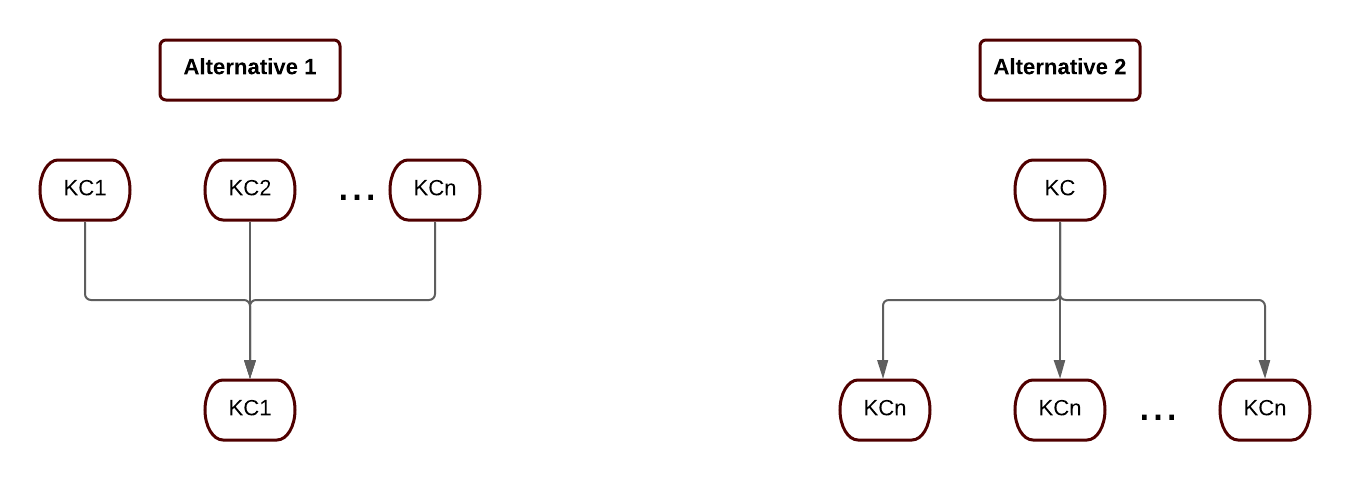
\includegraphics[width=\textwidth]{images/chapitre2/Two_Aggregation_relationships.png}
	\end{center}
\caption{Deux alternatives pour modéliser les relations d'agrégation.}
\label{two_agregationrelationships}
\end{figure}

Tchétagni et Nkambou ont proposé d’évaluer les connaissances des apprenants en logique propositionnelle à plusieurs niveaux de granularité. Ils ont utilisé le modèle alternatif 2 de la figure \ref{two_agregationrelationships} pour représenter les relations d'agrégation dans leur hiérarchie. Ils ont souligné que dans cette architecture, il existe des restrictions sur la façon dont les preuves se propagent dans tout le réseau. Cela est dû au fait que deux nœuds enfants peuvent influencer leur parent, sans s'influencer mutuellement : ils sont séparés. [15] \\
Carmona et Conejo ont utilisé dans la figure \ref{two_agregationrelationships} le modèle alternatif 1 pour représenter les relations d'agrégation dans leur modèle d'apprenant utilisé dans MEDEA, un système ouvert pour le développement de systèmes de tuteurs intelligents. Certaines approches récentes ont abordé la granularité du modèle de compétences d'un point de vue statistique. 

Dans ces approches, les modèles de compétences n'impliquent que les éléments de connaissance les plus fins, qui expliquent directement les comportements des apprenants. Un problème permanent dans un modèle d’apprenant est de savoir à quel niveau de granularité les compétences des apprenants doivent être modélisées. [16] Pardos et Heffernan ont exploré des modèles avec différents niveaux de granularité (modèles de compétences 1, 5, 39 et 106) et mesuré la précision de ces modèles en prédisant la performance des apprenants dans leur SIT, c'est-à-dire ASSISTment, ainsi que dans un test. Leurs résultats ont montré que plus la granularité du modèle de compétence est fine, meilleure est la prédiction des performances de l'apprenant. [17]

\subsection{Relations pré-requises}
Des relations préalables existent généralement entre les éléments de connaissance de certains domaines. \\
Reye a analysé comment utiliser les réseaux bayésiens pour modéliser les relations antérieures. Ils ont déclaré que les probabilités conditionnelles dans un réseau bayésien devraient remplir certaines conditions. Par exemple, si la composante de connaissance A est une condition préalable de la composante de connaissance B, l'équation II.1 doit être satisfaite. Cependant, ils ont également déclaré que la relation préalable n'est pas toujours stricte, de sorte qu'ils permettent une incertitude pour les probabilités conditionnelles. Les valeurs d'incertitude pour ces probabilités conditionnelles sont spécifiées par des experts dans leur méthode. [18]
\begin{equation}
	\begin{split}
		P(learnerKnows(A) \vee  learnerKnows(B)) = 1\\
	P(learnerKnows(B) \vee learnerKnows(A)) = 0
	\end{split}
\end{equation}
Carmona et al. ont présenté les relations préalables à un modèle générique d'apprentissage du BN pour MEDEA, afin d'améliorer l'efficacité des mécanismes d'adaptation et le processus d'inférence. Ils ont utilisé une porte ET bruyante modifiée ou une porte OU bruyante modifiée pour modéliser les relations de prédicat. [19] \\
Ferguson et al ont utilisé l'algorithme EM pour apprendre les paramètres cachés dans les BN et ont comparé le modèle de compétence plat (les compétences sont mutuellement indépendantes) avec le modèle de compétence hiérarchique (relations a priori entre des compétences données a priori) selon le critère d'information bayésien (BIC). Leurs résultats montrent qu'un modèle hiérarchique correspond mieux à leurs données que le modèle plat. [20]

\begin{figure}[H]
	\begin{center}
		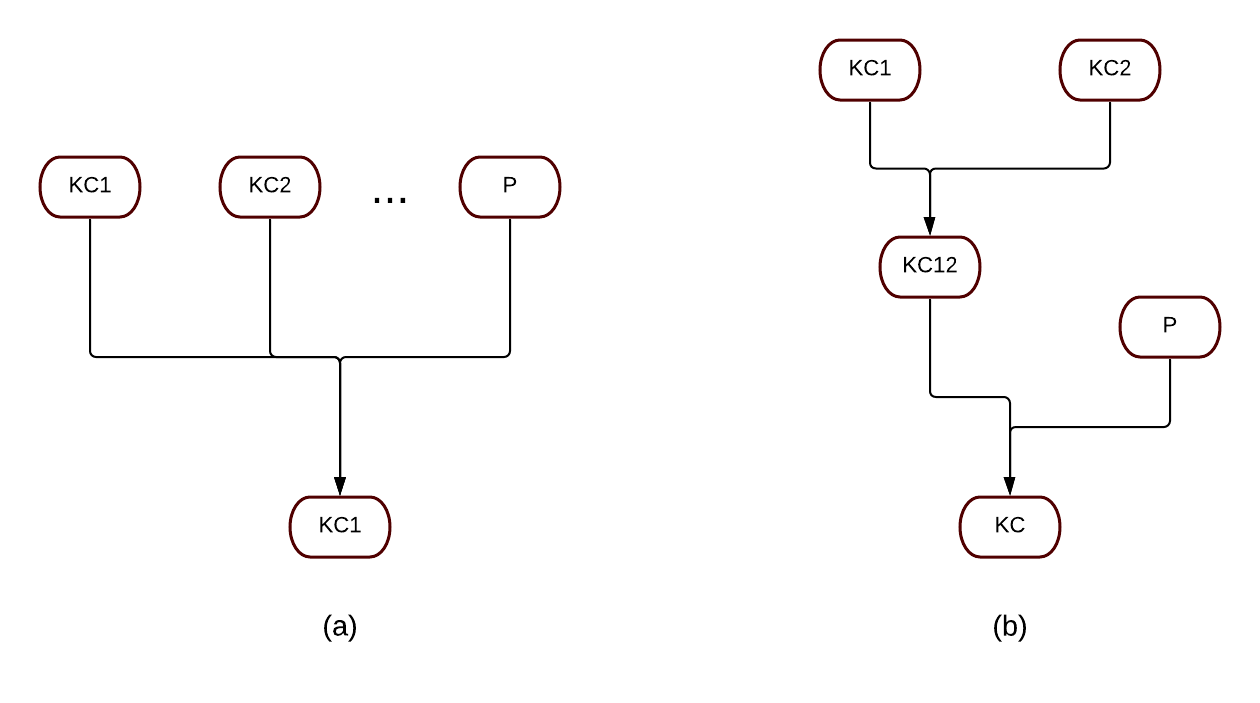
\includegraphics[width=\textwidth]{images/chapitre2/aggregationModelisation.png}
	\end{center}
\caption{Agrégation de modélisation de réseau bayésien et relations préalables simultanément}
\label{agregationModelisation}
\end{figure}

Millan et coll. discuté d'un problème courant dans la modélisation des apprenants, à savoir modéliser simultanément les relations de pré-requis et de granularité. Si les deux sont inclus dans le même modèle, les relations avec des interprétations différentes sont mélangées et il est alors difficile de construire et de comprendre le modèle. Par exemple, si une compétence KC composite est composée de deux sous-compétences, KC1 et KC2, il existe également une compétence P qui est un prérequis pour KC. Les probabilités conditionnelles de K données à ses parents sont difficiles à préciser (figure 1.3 (a)). Ils ont proposé une solution qui consiste à regrouper des variables de même type en introduisant des variables intermédiaires (figure 1.3 (b)). [21]

\section{Découverte des prérequis}
Nous modélisons les compétences comme des variables continues qui représentent le degré auquel un apprenant a maîtrisé ou est conscient d'une compétence particulière. Nous traitons les éléments comme des variables continues qui reflètent le degré auquel un apprenant a correctement terminé une tâche. En pratique, la mesure de l'achèvement des tâches est souvent une variable binaire avec des valeurs = correct / incorrect. Un élément binaire peut cependant être considéré comme une projection d'un élément continu, et les corrélations entre éléments continus idéalisés peuvent être estimées en calculant la matrice de corrélation tétrachorique parmi les éléments binaires mesurés. [22]

\begin{figure}[H]
	\begin{center}
		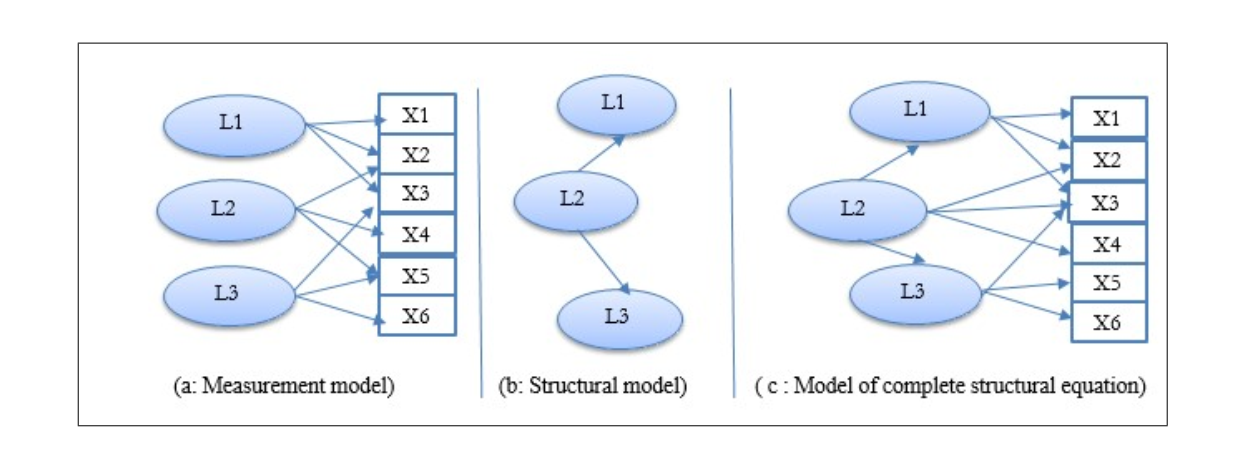
\includegraphics[width=\textwidth]{images/chapitre2/Modèles d'équations structurelles.png}
	\end{center}
\caption{Modèles d'équations structurelles}
\label{modeleEquation}
\end{figure}

L'utilisation de la matrice Q consiste généralement à définir quels éléments « chargent » sur quelles compétences latentes. Nous pouvons définir un « modèle de mesure » qui relie les compétences latentes aux items mesurés \ref{modeleEquation}. En modélisant les relations entre les compétences comme un modèle analytique causal du chemin entre les variables latentes \ref{modeleEquation}, appelé « modèle structurel », nous pouvons combiner le « modèle de mesure » et le « modèle structurel » pour former un modèle d'équation structurelle linéaire complet \ref{modeleEquation}. [23] \\
En supposant que le modèle de mesure est connu, nous pouvons rechercher le modèle structurel avec l'algorithme de découverte causale PC, dans lequel les entrées sont les relations d'indépendance et d'indépendance conditionnelle qui figurent parmi les variables latentes. Nous calculons ou testons les relations d'indépendance entre les latents en construisant un modèle structurel séparé et en l'ajustant aux données pour chaque test d'indépendance particulière requis. Notre méthode de construction de modèle produit un test cohérent et éprouvé de chaque relation d'indépendance conditionnelle. [22]

\section{Conclusion}
Tout au long de ce chapitre, nous avons présenté les principaux concepts liés au modèle de l'apprenant dans l'environnement de l'apprentissage basé sur le Web, qui permet aux apprenants de travailler en collaboration sur un projet ou de coconstruire le sens des concepts en utilisant la technologie comme un tuyau pour le développement des connaissances partagées, aussi, la modélisation des compétences est importante pour découvrir les prérequis d'un apprenant en représentant le degré auquel il a maîtrisé.
Le prochain chapitre sera consacré à la présentation de l'exploration de données éducatives.









\chapter{L'approche items-to-skills mapping} 
\minitoc
\thispagestyle{empty}
\newpage
\section{Introduction}
Les systèmes éducatifs contiennent un grand nombre d'items (problèmes, questions). Ces éléments sont proposés aux apprenants à résoudre. Ceci est particulièrement vrai pour les systèmes adaptatifs, qui tentent de présenter des éléments adaptés à différents types d'apprenants. La gestion d’un grand nombre d’éléments est très difficile. Ainsi, les systèmes éducatifs collectent des données sur les performances des apprenants et ces données peuvent être utilisées pour obtenir un aperçu des propriétés des éléments. [1] \\
Dans ce chapitre, nous présentons les approches pour mapper les éléments aux compétences. En outre, nous décrivons les concepts de l'approche de similarité avec ses différentes catégories, et nous représentons les différentes mesures de similitude telles que Pearson, Kappa, Yule et Fisher.
\section{Knowledge (La connaissance)}
\subsection{Définition}
"Compréhension ou information sur un sujet que vous obtenez par expérience ou étude, soit connue par une personne ou par des personnes". [Dictionnaire Cambridge] La « connaissance » en éducation est constituée de faits de base alors que les composants de connaissance peuvent être des procédures, des schémas d'intégration, des stratégies de raisonnement complexes, des compétences métacognitives ..., c'est-à-dire (1er niveau de la taxonomie de Bloom (1956)). \\
La « connaissance » en philosophie est une « croyance vraie justifiée » alors que notre utilisation des éléments de connaissance comprend à la fois une connaissance incorrecte (fausse) et une connaissance implicite (sans croyance ou justification explicite). [2]

\subsection{Knowledge component (Composante connaissance)}
Un élément de connaissance est une description d'une structure mentale ou d'un processus qu'un apprenant utilise, seul ou en combinaison avec d'autres éléments de connaissance, pour accomplir les étapes d'une tâche ou d'un problème. (Koedinger, Corbett \& Perfetti, 2012) Les items qui requièrent la même compétence pour différents apprenants constituent une composante de connaissance (KC) [3]. \\
Composante de connaissance est un terme que nous utilisons tous les jours comme concept, principe, fait ou compétence, et des termes de sciences cognitives comme schéma, règle de production, idée fausse ou facette. [4]
La description de la composante de connaissance est présentée dans la figure \ref{knowledge_component}.

\begin{figure}[H]
	\begin{center}
		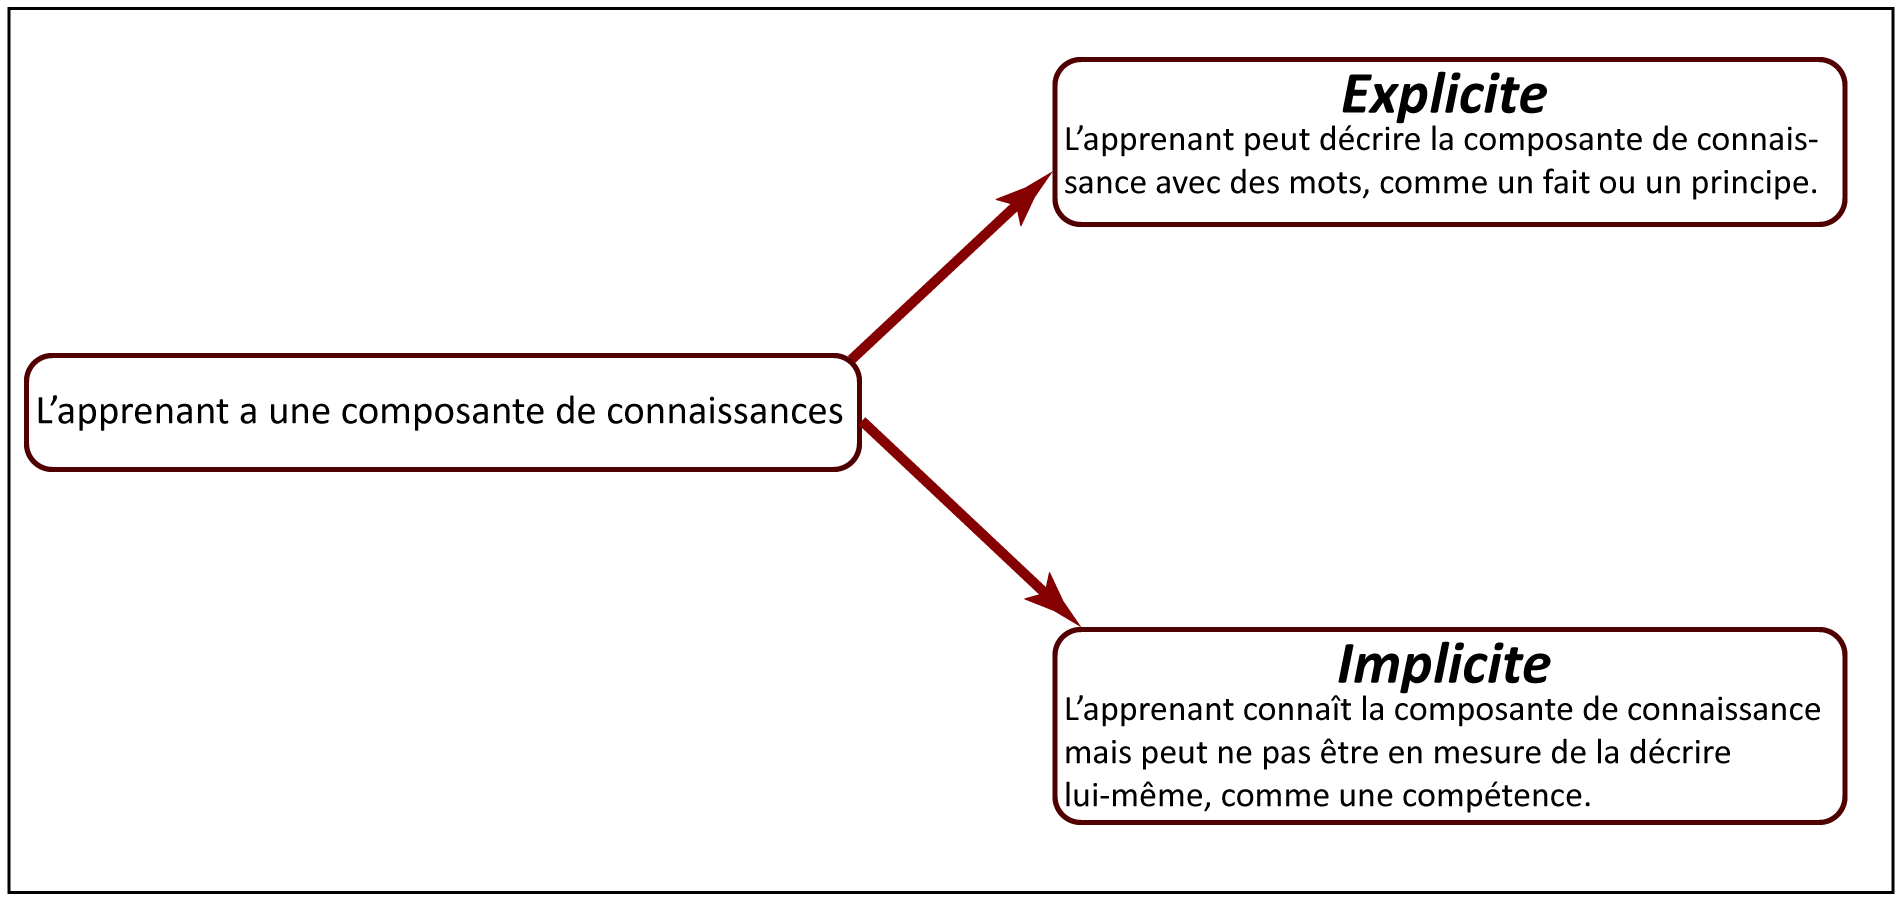
\includegraphics[width=\textwidth]{images/chapitre3/Knowledge_component.png}
	\end{center}
\caption{Knowledge Component}
\label{knowledge_component}
\end{figure}
\textbf{\underline{Exemple :}}
"Si l'angle A = 60 et (A = B, C = 60) Alors triangle équilatéral." \\
L'élève peut dessiner un triangle équilatéral sans être capable de décrire la règle. Une grande partie de ce que les apprenants de première langue savent de leur langue maternelle implique des éléments de connaissances implicites. Pertinence : la plupart des composants de connaissance explicites impliquent de nombreux composants de connaissance tacites (compétences innées ou acquises, le savoir-faire et l'expérience). La réponse et la fonctionnalité sont liées par la composante de connaissance, où les deux peuvent être externes, dans le monde, comme des signaux dans un stimulus et une réponse motrice ou interne, dans l'esprit, comme des fonctionnalités inférées et un nouvel objectif. [4].

\subsection{Les types de composante de connaissance}

La composante de connaissance est une représentation mentale de : [5]

\begin{itemize}
    \item[$\bullet$] \textbf{Connaissance du domaine :} faits, concepts, principes, règles, procédures, stratégies.
    \item[$\bullet$] \textbf{Connaissances préalables :} connaissance de l'encodage des fonctionnalités.
    \item[$\bullet$] \textbf{Connaissance intégrative :} schémas ou procédures qui connectent d'autres KC.
    \item[$\bullet$] \textbf{Connaissances métacognitives :} sur les connaissances, le contrôle de l'utilisation ou l'acquisition des connaissances.
    \item[$\bullet$] \textbf{Croyances et intérêts :} ce que l'on aime, croit.
    \item[$\bullet$] \textbf{Toute représentation externe des connaissances :} (comme les descriptions de manuels ou un exemple) ou les structures cognitives génériques (mémoire de travail), soit, les paramètres continus sur les représentations des connaissances (force, niveau d'engagement, valeur implicite d'un objectif, affect) ne sont pas des composants de connaissances.
\end{itemize}

\section{Items-to-skills mapping}
\subsection{Définition}
Mapper les éléments aux compétences latentes est l'automatisation de la découverte des compétences derrière les éléments de question à des fins d'ingénierie cognitive est hors de portée dans l'état actuel de la recherche, des moyens pour aider à déterminer le nombre de compétences et les compétences communes entre les éléments est un effort raisonnable au milieu -terme. [6]

\subsection{items-to-skills mapping Structure}
Il existe deux approches de la cartographie des éléments aux compétences présentées dans la figure \ref{items_to_skills_mapping}:

\begin{figure}[H]
	\begin{center}
		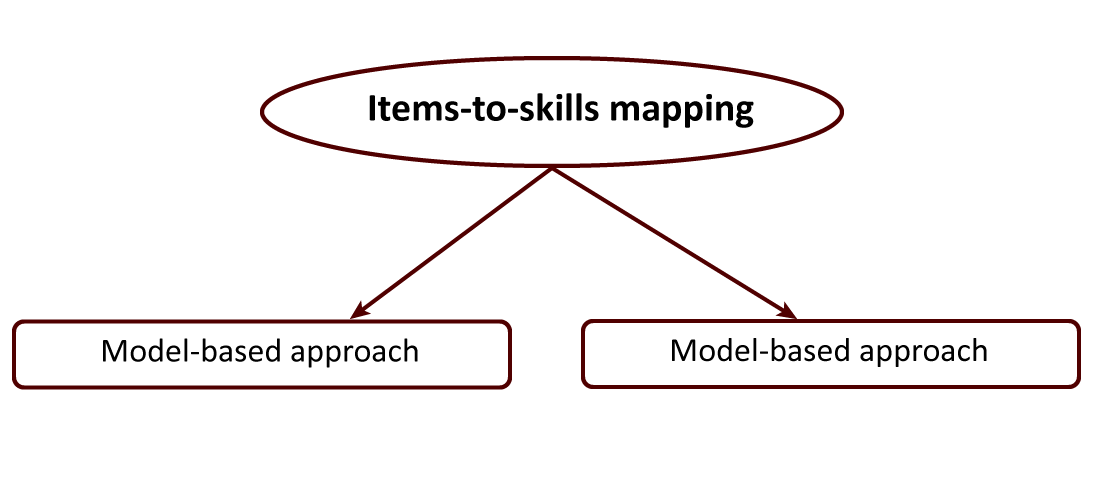
\includegraphics[width=\textwidth]{images/chapitre3/Items_to_skills_mappin_structure.png}
	\end{center}
\caption{Items-to-skills mapping Structure}
\label{items_to_skills_mapping}
\end{figure}

\subsubsection{Model-Based approach}
\paragraph{Définition}
La construction d'un modèle simplifié qui explique les données observées. Basé sur une matrice de réponses des apprenants aux éléments, le modèle prédit les réponses de l'apprenant. Le modèle attribue plusieurs compétences latentes aux apprenants et utilise une cartographie des éléments aux facteurs latents correspondants. Ce type de modèle peut souvent être exprimé naturellement à l'aide de la multiplication matricielle, c'est-à-dire que l'ajustement d'un modèle conduit à une factorisation matricielle. Une fois que nous obtenons le résultat après avoir ajusté le modèle aux données, nous avons désigné les items avec la même valeur d'un facteur latent comme « similaires ». Cette approche conduit naturellement à plusieurs composantes de connaissance par compétence. [1] Le modèle basé sur le modèle présenté dans la figure \ref{model_based} développe un modèle de notation des utilisateurs, les algorithmes de cette catégorie adoptent une approche probabiliste en calculant la valeur attendue de la prédiction de l'utilisateur et en tenant compte des notes de l'utilisateur sur d'autres éléments. [8] \\
Le processus de modèle peut être produit par différents algorithmes d'apprentissage automatique tels que le réseau bayésien, le clustering et l'approche basée sur des règles. [7]

\begin{figure}[H]
	\begin{center}
		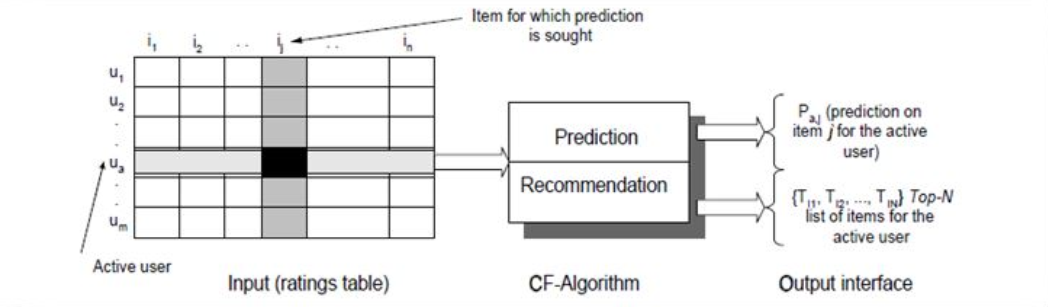
\includegraphics[width=\textwidth]{images/chapitre3/Model_based.png}
	\end{center}
\caption{Model based}
\label{model_based}
\end{figure}

Cette approche guide des composants de connaissances différents et multiples par compétence. Le modèle est généralement calculé à l'aide d'une technique d'optimisation qui ne mène qu'à des optima locaux (par exemple, une descente de gradient). \\
Dans les systèmes recommandés, cette approche est utilisée pour la mise en œuvre du filtrage collaboratif ; elle est souvent appelée "Décomposition en valeurs singulières" (SVD). [9] 

\paragraph{Model Based Techniques}
Dans le contexte pédagogique, de nombreuses variantes de l'approche basée sur les modèles ont été proposées : \\

\begin{itemize}
    \item[$\bullet$] \textbf{Q-matrix :} Est une matrice binaire illustrée à la figure 4 montrant la relation entre les éléments de test et les attributs ou concepts latents ou sous-jacents (Birenbaum, et al., 1993). Les états de connaissance ont été attribués aux apprenants en fonction de leurs réponses aux tests et de la matrice q construite. [10]
\end{itemize}

\begin{figure}[H]
	\begin{center}
		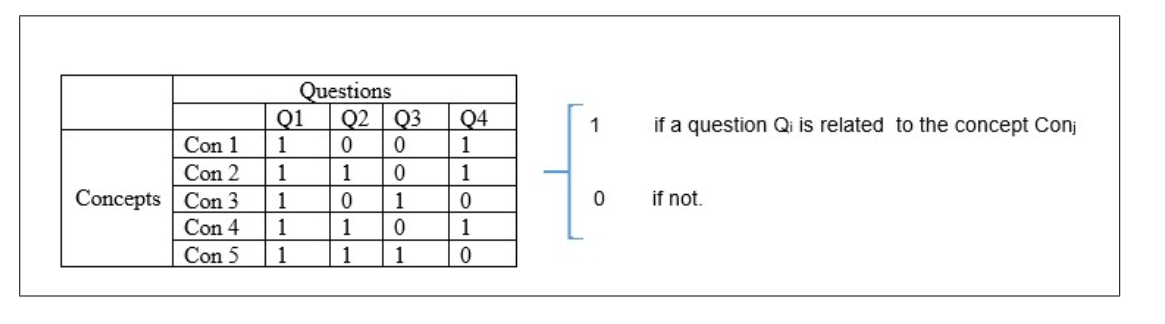
\includegraphics[width=\textwidth]{images/chapitre3/q_matrix.png}
	\end{center}
\caption{Q-matrix}
\label{q_matrix}
\end{figure}

\subsection{Similarity-based approach (Item-Similarity)}
\subsubsection{Définition}
En statistiques et en mathématiques, la mesure de similarité ou la fonction de similarité est une fonction à valeur réelle qui mesure la similarité entre deux éléments. Les valeurs de similarité entre les éléments sont quantifiées par l'observation de la performance des utilisateurs sur les éléments, qu'il s'agisse de négatif ou non [11]. La mesure des similitudes est une étape très importante dans une analyse plus approfondie telle que le regroupement des éléments, ce qui est utile à plusieurs égards. [12]  \\
Dans cette approche, nous calculons directement une mesure de similarité pour chaque paire d'éléments. Ces similitudes sont ensuite utilisées pour faire le clustering, pour faire la visualisation en projetant ces éléments dans un plan a 2 ou 3 dimensions, ou pour faire d’autre analyse en essayant de récupérer les éléments les plus similaire. Cette approche est illustrée à la figure \ref{illustration_item_similarity}. 

\begin{figure}[H]
	\begin{center}
		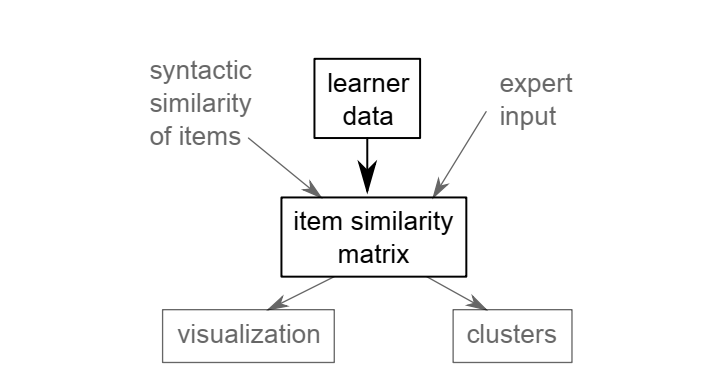
\includegraphics[width=\textwidth]{images/chapitre3/Illustration_item_smilarity.png}
	\end{center}
\caption{Illustration de l'approche générale de l'analyse des éléments basée sur les similitudes des éléments.}
\label{illustration_item_similarity}
\end{figure}

Dans l'apprentissage éducatif, la définition de la similarité des éléments a été analysée en utilisant la corrélation des réponses des apprenants et les temps de résolution des problèmes, ainsi qu'en utilisant les mauvaises réponses des apprenants. [12]

\subsubsection{Processus de similarité des items (éléments)}
Une étape importante de l'approche basée sur les items consiste à calculer le degré de similitude entre chaque paire d’items, puis à sélectionner les éléments les plus similaires. Il peut être décrit comme l'opération de calcul de similarité entre deux éléments i et j, où il s'agit d'abord de définir les utilisateurs qui ont évalué ces deux éléments, puis d'appliquer une technique de calcul de similarité pour déterminer le score de similarité entre i et j. [13] La figure \ref{calcul_application_similarity} ci-dessous montre l'approche générale du calcul et de l'application de la similarité des items.

\begin{figure}[H]
	\begin{center}
		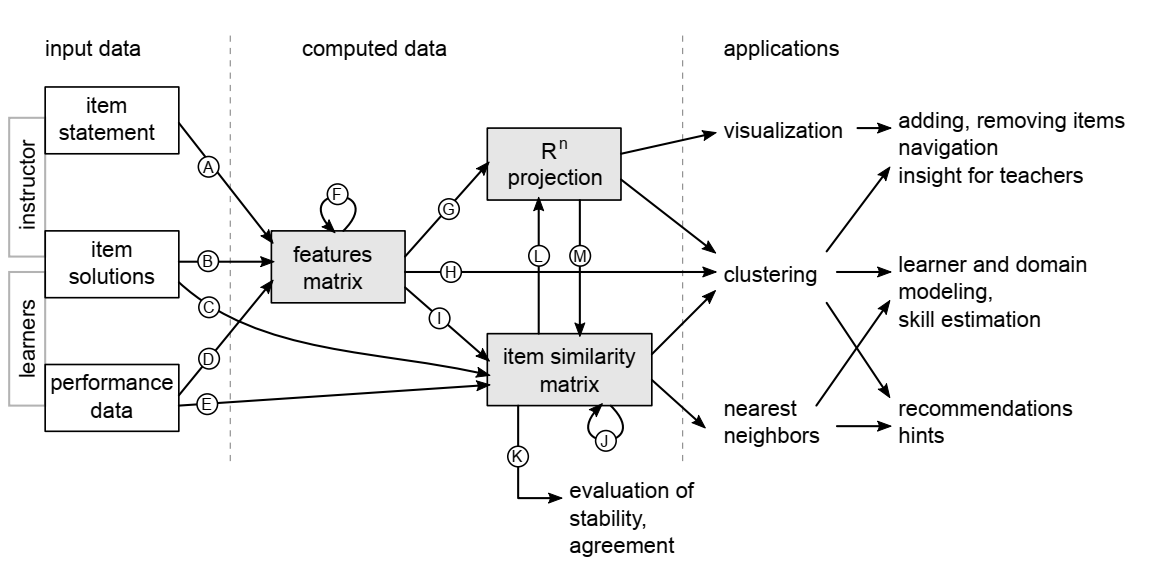
\includegraphics[width=\textwidth]{images/chapitre3/calcul_application_similarity.png}
	\end{center}
\caption{L'approche générale du calcul et de l'application de la similarité des éléments.}
\label{calcul_application_similarity}
\end{figure}

Nous allons brièvement parcourir les trois étapes input data, computed data, applications illustrées dans la figure \ref{calcul_application_similarity}. 
\paragraph{Input Data}

\begin{itemize}
    \item \underline{Item statement (Arrow A) :} Un énoncé d'item dans est la spécification de la tâche que l'apprenant doit résoudre donnée en langage naturel, ou des exemples d'entrée-sortie.
    
    \begin{itemize}
		\item La construction de la matrice des fonctionnalités nécessite d'abord un prétraitement à l'item qu'il soit en langage naturel,
		\item Les techniques du modèle du sac de mots qui permettent par exemple de représenter le texte par un vecteur avec le nombre d'occurrences de chaque mot
		\item D'autres caractéristiques peuvent être obtenues à partir de la spécification des données d'entrée, par exemple, les types de variables (entier, chaîne, liste)
	\end{itemize}
	
\end{itemize}

\begin{itemize}
    \item \underline{Item solution} Est simplement la solution donnée par l’apprenant ou la solution commune des apprenants. Elle est présentée comme un programme dans un langage de programmation donné.
    
    \begin{itemize}
		\item Feature Matrix : (Arrow B)
		\begin{itemize}
			\item Analyse du code source jusqu'aux fonctions de calcul décrivant l'apparition des concepts de programmation et des mots-clés (alors, if, return,print, ) soit l'utilisation d'opérateurs.
			\item Le modèle du sac de mots est appliqué uniquement sur les mots-clés de programmation au lieu de mots dans un langage naturel.
		\end{itemize}

		\item Direct computation of similarities: (Arrow C)
		\begin{itemize}
			\item Le calcul de la distance entre les solutions choisies des deux items.
			\item Il est calculé par plusieurs méthodes, par exemple : distance d'édition d'arbre d'exemple pour l'arbre de syntaxe abstraite, ou la distance d'édition de base de Levenshtein pour le code canonisé.
		\end{itemize}
	\end{itemize}
	
\end{itemize}

\begin{itemize}
    \item \underline{Performance data} Informations sur la performance des apprenants lors de la résolution des items par exemple : exactitude de la réponse, temps de réponse, nombre d'indices utilisés et nombre de tentative faite sur un seul item.
    
    \begin{itemize}
		\item Feature matrix (Arrow D) : Les données sont transformées en fonctionnalités telles qu'un écart de performance ou le ratio d'apprenants qui ont résolu l'élément correctement.

		\item Direct computation of similarities: (Arrow E)
		\begin{itemize}
			\item La similitude des items i, j est le résultat du calcul de leur corrélation basé sur les performances des apprenants qui ont résolu les items i et j.
			\item Il peut être calculé en utilisant la méthode de correction (réponse correcte/incorrecte) ou la méthode des temps de résolution (plutôt que la correction).
		\end{itemize}
	\end{itemize}
	
\end{itemize}

\paragraph{Computed Data}

\begin{itemize}
    \item \underline{Features matrix :} c'est la matrice qui contient les éléments et leurs caractéristiques qui peuvent être par exemple une solution d'élément ou des mots-clés apparaissant dans une déclaration d'élément. La matrice de caractéristiques peut être normalisée ou transformée (flèche F) à l'aide de techniques telles que la transformation terme fréquence-fréquence inverse du document. La matrice de caractéristiques peut être normalisée ou transformée (flèche F) à l'aide de techniques telles que la transformation terme fréquence-fréquence inverse du document.A partir de la matrice de caractéristiques, nous pouvons calculer une projection sur Rn (flèche G et flèche L). La projection est généralement utilisée pour des applications, en particulier pour la visualisation d'éléments. Cependant, cela peut également être une étape de traitement utile dans le calcul des similitudes d'articles, par exemple, pour décorréler des caractéristiques.
	\item \underline{Item similarity matrix :} est une matrice bidimensionnelle m, où m[i,j] désigne la similarité des items i et j. Le calcul de la matrice de similarité basée sur la matrice de caractéristiques (flèche I) ou sa projection dans Rn (flèche M) est une opération courante en apprentissage automatique, avec de nombreux choix disponibles, par exemple la similarité cosinus, le coefficient de corrélation de Pearson et la distance euclidienne (transformé en mesure de similarité par soustraction).
\end{itemize}

\subsubsection{Item-Similarity measures}
Pour calculer le score de similarité entres deux items, il faut tout d’abord créer la matrice d’accord entre item i et item j. Cette matrice d’accord appeler aussi matrice de confusion ou (confusion matrix en anglais) est illustrer par le tableau 3.

\begin{table}[!htbp]
    \centering
	\begin{tabular}{|c| c|c|}
	\hline
	 & Item i (Correct) & Item i (Incorrect)  \\ \hline
	 Item j (Correct) & a & b  \\  \hline
	 Item j (Incorrect) & c & d  \\  \hline
	\end{tabular}
	\caption{La matrice d’accord pour deux items}
	\label{matrice_accord}
\end{table}

Ensuite cette matrice d’accord est utilisée pour calculer la similarité entre l’item i et j. Les coefficients de calcule de similarité qui peuvent être utiliser sont les suivants (Figure 4) :

\begin{table}[!htbp]
    \centering
	\begin{tabular}{|c| c|}
	\hline
	Mesures & Equation  \\ \hline
	Yule  & \(\displaystyle Sy = (ad-bc)/(ad+bc)\)   \\  \hline
	Pearson  &  \(\displaystyle Sp = (ad-bc)/\sqrt{(a+b)(a+c)(b+d)(c+d)}\) \\ \hline
	\makecell{\\Cohen \\ \\ \\}  & \makecell{\(\displaystyle Sc = (Po-Pe)/(1-Pe) \) \\ \(\displaystyle Po = (a+d)/n\) \\  \(\displaystyle Pe = ((a+b)(a+c)+(b+d)(c+d))/n^{2} \)}  \\  \hline
	Sokal  & \(\displaystyle Ss = (a+b)/(a +b +c + d)  \)   \\  \hline
	Jaccard  & \(\displaystyle Sj = a/(a+b+c) \)   \\  \hline
	Ochiai  & \(\displaystyle So = a/\sqrt{(a+b)(a+c)} \)   \\  \hline
	\end{tabular}
	\caption{Ccv}
	\label{differentes_mesures_similarité}
\end{table}

\section{Conclusion} 
Dans ce chapitre nous avons a introduit les concepts de base de la composante connaissance, la cartographie des approches des compétences, en spécifiant différentes similitudes qui peuvent ensuite être utilisées dans une analyse plus approfondie des relations d'un élément, telles qu'un regroupement d'éléments ou une visualisation. Ensuite, la revue de la littérature et les travaux connexes dans le domaine de l'apprentissage profond et de l'exploration de données éducatives.
%\chapter{Le Deep Learning et les Techniques de Détection d'intrusions}
\minitoc
\thispagestyle{empty}
\newpage	
	
	\section{Introduction}
Comme nous l'avons vu dans les chapitres précédents qu'une fois que les appareils connectés à l'Internet, ils deviennent vulnérables à d'éventuelles attaques informatiques et avec la croissance du nombre d'objets connectés ainsi que les menaces dont fait face l'IoT, il est fortement primordial d'assurer la sécurité des données et des objets connectés.\\  
	La meilleure façon de protéger un réseau ou un système informatique est de détecter les attaques et de se défendre avant même qu’elles ne se produisent. Pour cela beaucoup font appel aux systèmes de détection d’intrusion(IDS) et des systèmes de prévention d'intrusions (IPS) afin de détecter les attaques que peut subir une machine ou le réseau.\\Ces systèmes de surveillance du réseau et des hôtes sont devenus pratiquement indispensables dû à l'incessant accroissement en nombre et en dangerosité des attaques ces dernières années.
	
Par exemple pour assurer l'intégrité des maisons et la sécurité de leurs propriétaires certaines personnes équipent leurs  maisons de systèmes d'alarme qui se déclenchent pour prévenir les propriétaires ou les autorités contre toute effraction ou intrusion dans la maison. \\
De même que le système d'alarme signale l'intrusion dans une maison, le système de détection d'intrusion signale aussi l'intrusion dans une machine ou dans un réseau.\\    

Les systèmes de détection d'intrusion tiennent leur origine de l'armée Américaine qui a initié pour la première fois les techniques de détection d’intrusions en 1980 \cite{refids}. Par la suite plusieurs projets de recherches sur le sujet ont vu le jour dont certains furent couronnés de succès. Avec l'apparition du machine learning et du deep learning de récents travaux utilisant ses techniques d'apprentissages intelligentes ont données des résultats promettants \cite{refidsann} \cite{6664371} \cite{articleids}.\\
  
  Dans ce chapitre, nous présentons premièrement les systèmes de détection d'intrusion, ses diverses caractéristiques, les différents types d'IDS. Ensuite nous exposons le Deep Learning, son origine et ses différents modèles. Enfin on présentera notre approche résiliente pour l'identification et la détection des attaques DDoS dans les réseaux IoT basée sur les modèles de Deep Learning.	
	\section{systémes de détection d'intrusion}
	\subsection{Définition }
Un Système de détection d'intrusion(IDS) est un composant logiciel ou matériel spécialisé, dont le rôle est de surveiller l'activité d'un réseau ou d'un hôte en vue de détecter toute effraction dans l’utilisation des ressources.\\
L’ef{\kern0pt}fraction ou l’intrusion est définie comme une pénétration illégale dans un système, une tentative d’un utilisateur du système d'obtenir des privilèges non autorisés, ou bien toute tentative de viol de la politique de sécurité \cite{zaidi}. Cela veut dire qu'elle peut être d'origine intérieure ou  d'origine extérieure.\\

Vu l'évolution de la complexité des attaques et l'hétérogénéité du trafic des objets connectés ainsi que les dif{\kern0pt}férents paramètres entrant en jeu dans le processus de détection, la détection des intrusions devient une tâche très complexe. Néanmoins, il existe plusieurs travaux de recherches qui ont abouti à de multiples approches et de résultats promet{\kern0pt}tants.
\subsection{Architecture de base d'un IDS}
Plusieurs architectures ont été proposées pour décrire les dif{\kern0pt}férents éléments intervenants dans un système de détection d’intrusion. Il y a trois modules communs à la majorité des architectures IDS proposées\cite{zaidi} : la source de données, l’analyseur des données et le module des réponses.
\begin{itemize}
\item\textbf{la source de donnnées :} ou senseur joue le rôle de collecteur d'informations, telles que les données de trafic sur le réseau ou les données log et les transmet ensuite à l'analyseur. Un IDS peut contenir plusieurs senseurs qui doivent être placée à une position stratégique pour une meilleure qualité de détection du système.
\item\textbf{L'analyseur :} son rôle est d'analyser les données reçues des senseurs et indiquer s'il y a eu anomalie ou pas.
\item\textbf{Le module de réponse :} comme son nom l'indique, il s'occupe de la réponse de l'IDS face aux anomalies détectées. Ça peut être un simple message d’alerte, une sauvegarde dans un fichier log ou bien une interruption de la connexion.   
\end{itemize}
\subsubsection{Architecture CIDF}
Le Common Intrusion Detection Framework (CIDF) est un effort visant à développer des protocoles et des interfaces de programmation d'application afin que les projets de recherches sur la détection d'intrusion puissent partager des informations et des ressources pour que les composants de détection d'intrusion puissent être réutilisés dans d'autres systèmes \cite{refcief}.
L'architecture CIDF, utilise quatre modules : Générateur d'événements, Analyseur d'événements, Unité de réponse et une Base de données d'événements. Les trois premiers modules jouent les mêmes rôles que ceux cités dans la section précédente. Tandis que la Base de données des événements est utilisée pour le stockage des évènements et des données analysées \cite{zaidi}
\cidf
\subsubsection{L’architecture IDWG}
Dans l'architecture proposée par le groupe Intrusion Detection exchange format Working Group (IDWG) de l'IETF, on trouve les trois modules cités précédemment couplés avec d’autres composants. Dans cette architecture, l’objectif était la définition d’un standard de communication entre les composants d'un IDS. Cette architecture définit un format d'échange de message pour les IDS. 
\idwg
Cette architecture est composée des modules suivants\cite{zaidi} :
\begin{itemize}
\item \textbf{source de données :} c’est l’interface entre le système surveillé et l’IDS, elle fait la collecte d’informations sur les activités du système.
\item \textbf{Capteur :}chargé de filtrer et de formater les informations brutes envoyées par la source de données. Le résultat de ce traitement sera un message formaté, appelé aussi événement, il représente l'unité de base dans un scénario d'attaque.
\item \textbf{Analyseur :} permet d’analyser les évènements générés par le capteur. S’il détecte une activité intrusive, il émet une alerte qui est un message sous un format standard. Dans cette architecture, le capteur et l’analyseur forment ensemble une sonde.
\item \textbf{Manager :}en plus de la notification des alertes, il offre à l’administrateur la possibilité de configurer une sonde et de gérer les alertes envoyées par l’analyseur.
\end{itemize} 
\subsection{Classification des systèmes de détection d'intrusion}
Les IDS peuvent être classés selon leur architecture, la provenance de leurs données ainsi que selon leur approche de détection et de réponse\cite{articletypeids}. La figure \ref{ids} résume ses dif{\kern0pt}férents types d'IDS\label{classification}
\typeids
\subsubsection{L’emplacement d’IDS }
%généralement placée derrière le par-feu pour une meilleur
Il existe trois types d'IDS selon l'emplacement de la source de l'information où ils opèrent. Ces sources d'information représentent les paquets capturés à partir des réseaux, des fichiers des systèmes d'exploitation, des logiciels ou encore à partir des fichiers log.
\paragraph{Détection d'intrusion basée sur l'hôte (HIDS) : }
Un système de détection d'intrusion basé sur l'hôte est un IDS spécifique à un hôte unique. il analyse exclusivement l'information concernant cet hôte et surveille son système contre les attaques internes et externes. 
L'IDS est installé sur le système lui-même, une Position idéal pour filtrer avec précision l'ensemble du trafic venant d'extérieur vers cet hôte. 
Les HIDS sont en général placés sur des machines sensibles, susceptibles de subir des attaques et possédantes des données sensibles pour l’entreprise.
\hids
\paragraph{ Détection d'Intrusion basée sur une application (AIDS):} 
Les IDS basés sur les applications (AIDS) sont un sous-groupe des IDS
hôtes. Ils contrôlent l'interaction entre un utilisateur et une application en ajoutant des fichiers log afin de fournir de plus amples informations sur les activités d'une application particulière. Un AIDS se situe
au niveau de la communication entre un utilisateur et l’application surveillée.
L’avantage de cet IDS est sa capacité de détecter et d’empêcher des
commandes particulières dont l'utilisateur pourrait se servir avec le programme et
de surveiller chaque transaction entre l’utilisateur et l’application. De plus, les données sont décodées dans un contexte connu, leur analyse est donc plus fine et précise. Par contre, du fait que cet IDS n’agit pas au niveau du noyau, la sécurité assurée est plus faible, notamment l'attaques de type "Cheval de Troie". Ce type d’IDS est utile pour surveiller l’activité d’une application sensible, mais son utilisation s'effectue en général en association avec un HIDS. Il faudra dans ce cas contrôler le taux d’utilisation CPU des IDS afin de ne pas compromettre les performances de la machine.\cite{reftypeids}
\paragraph{ La Détection d'Intrusion Réseau (NIDS) :}
Un IDS basé sur le réseau est un IDS qui examine le trafic réseau en analysant les paquets par rapport à une base de données contenant des signatures d'attaques connues afin de détecter les anomalies. Il est défini juste à l'entrée du réseau ou entre le réseau et le serveur. L'avantage de cela est que ça permet d'analyser efficacement et rigoureusement le trafic venant de l'extérieur vers le réseau.\\ 
L'implantation d’un NIDS sur un réseau se fait de la façon suivante : des
capteurs sont placés aux endroits stratégiques du réseau et génèrent des alertes s’ils détectent une attaque. Ces alertes sont envoyées à une console sécurisée, qui les analyse et les traites éventuellement. Cette console est généralement située sur un réseau isolé, qui relie uniquement les capteurs et la console. Dans le cadre de réseaux IoT, l'IDS peut être placé au niveau de l'IoT gateway.
\nids
\subsubsection{Mode de détection }
Les systèmes de détection d'intrusion ont été conçu de telle sorte qu'ils puissent détecter et identifier efficacement les menaces.
Deux modes de détection ont été proposées : l'approche comportementale et la
reconnaissance de signatures.
\paragraph{L'Approche comportementale :}\label{comportement}
 La détection d'intrusion par l'approche comportementale consiste à détecter le comportement d'un trafic d'intrus(attaque) par rapport à un profil de trafic habituel(normal) en ce qui concerne la bande passante et le protocole. 
 \begin{comment}
 Sa mise en œuvre comprend : 
\begin{itemize}
\item envoie le jeu de donnée normale(le trafic normal)
\item  phase d'apprentissage au cours de laquelle les IDS apprennent le fonctionnement "normal" des entités surveillés.
\item phase de comparaison de tout le trafic réseau à ce comportement normal appris.
\item déclencher une alerte en cas d'une incohérence avec le comportement normal connu
À titre d’exemple, un projet très ambitieux a été sponsorisé par la DARPA (en 98 et 99), en collaboration avec le laboratoire Lincoln du MIT \cite{refdarpa}. L'objectif était de fournir un jeu de données d'apprentissage comprenant trafic de fond et activités intrusives (c’est-à-dire du trafic intrusif ou des événements systèmes causés par des attaques). Le trafic de fond était déduit des données statistiques collectées sur le réseau des bases de l’Air Force alors que les attaques étaient générées par des scripts créés spécialement, mais aussi par des scripts collectés à travers des sites spécialisés et des listes de diffusion. Les données collectées concernaient à la fois des HIDS et des NIDS.\\ 
\end{itemize}
\end{comment} 
Dans le cas du HIDS, ce type de détection peut être basé sur des informations telles que le taux d’utilisation CPU, l’activité sur le disque, les horaires de connexion ou d’utilisation de certains fichiers (horaires de bureau…).\\
\textbf{Avantages : } les IDS basés sur l'approche comportementale ont des capacités de détecter tous les types d'attaques y compris les Zéro day attaques.
Cette approche permet de produire l'information utile pour la définition des
signatures des IDS à base de signatures\cite{reftypeids}.\\
\textbf{Inconvénients :} Le grand défaut de cette approche est le grand nombre de fausses alertes dues aux comportements imprévisibles des utilisateurs du réseau. Elle exige souvent l’historique à long terme des évènements enregistrés afin de caractériser les modèles normaux de comportement \cite{reftypeids}.
\paragraph{La reconnaissance de signature :}
La détection d'intrusion basée sur la reconnaissance de signatures consiste à la détection d'attaques en recherchant des signatures spécifiques, tels que des séquences d'octets dans le trafic réseau ou des séquences d'instructions malveillantes connues utilisées par des logiciels malveillants. Une signature permet de définir les caractéristiques d’une attaque, au niveau des differentes couches protocolaires du modèle (TCP/IP). Ces signatures proviennent en général des antivirus qui donnent une signature spécifique à chaque types d'attaques. \\
C'est une approche qui utilise les connaissances accumulées sur les attaques spécifiques et les vulnérabilités du système
\begin{comment}
 Sa mise en œuvre comprend : 
\begin{itemize}
\item un jeu de donnée contenant les signatures des attaques connues
\item  phase d'apprentissage au cours de laquelle les IDS apprennent les signatures des attaques.
\item phase de comparaison des données des entités surveillés par rapport aux signatures des attaques connues.
\item déclencher une alerte en cas de similarité entre des données et la base de signature.
\end{itemize}
\end{comment}
\textbf{Avantages : } le plus grand avantage des systèmes de détection d'intrusion basés sur la reconnaissance de signature est qu'il détectent de façon très efficace les attaques dont ils disposent de leur signature sans produire un grand nombre de fausses alertes. \\ 
\textbf{Les inconvénients :}
Les IDS basés sur la reconnaissance de signature ne peuvent pas détecter les attaques dont ils ne possèdent pas les signatures. De ce fait, il nécessite des mises à jour fréquentes de sa base de signature.
Les pirates contournent facilement ces types d'IDS en utilisant les techniques dites "d'évasion" qui consistent à faire varier les signatures des attaques de tels sorte que les IDS ne les reconnaissent plus.
\subsubsection{Types de réponse}
les IDS étant des systèmes très réactifs donc chaque fois qu'une intrusion est détectée, le système déclenche une alerte. cette section décrit comment le système réagira à l'alerte déclenchée. Il existe deux types de réponses : réponse passive et réponse active.
La majorité des IDS existants fournissent une réponse passive. Par contre la réponse active est plus ou moins implémentée\cite{articlepa}.
\paragraph{ La réponse passive :}
La réponse passive d’un IDS consiste à enregistrer les intrusions détectées dans un fichier log qui sera analysé par l'administrateur du système. Cette réaction peut être aussi par l'envoie d'un email ou l'ouverture d'une fenêtre console contenant les détails de l'intrusion. Il est à noter que ce type d'IDS n’empêche pas directement une attaque de se produire, c'est à la charge de l'administrateur système de prendre la décision d'appliquer la politique de sécurité nécessaire pour empêcher l'intrusion de se produire. 
\paragraph{ La réponse active :} 
En plus d'être un IDS passif, Un IDS actif peut stopper une attaque au moment de sa détection. Pour cela, à la détection d'une attaque l'IDS prend des décisions pour modifier l'environnement du système attaqué sans l'intervention requise d'une personne. Cette altération peut consister à la déconnexion de l'attaquant ou la ré-configuration des mécanismes réseaux pour bloquer toutes les connections provenant de la même adresse source.
\subsubsection{La fréquence d'utilisation }
Le mode d'utilisation d'un IDS peut être choisi selon les besoins en fonction du mode d'utilisation : continue (online) ou périodique (offline). 
\paragraph{Utilisation continue :}
L'utilisation continue est une analyse en temps réel(online) c'est-à-dire la détection d'attaques se fait au moment où elle se produit. Le principal avantage est que les alertes sont lancées dès que les attaques sont détectées. Cet état de veille coute cher en termes de ressources et nécessite des algorithmes plus complexes que ceux d'une analyse différé.\cite{reftmqb} 
\paragraph{ Utilisation périodique :}
L'utilisation périodique est une analyse différé(offline) cela veut dire que L'analyse s'effectue sur des données stockées (non fraîches) dans des fichiers logs. Elle est préférable pour avoir une défense plus fiable du point de vue du temps de calcul. En effet pour un IDS online le temps de calcul de l'IDS doit être supérieur au temps du trafic réseau, ce qui est difficilement atteignable et peut affecter considérablement le trafic réseau.
\subsection{Exemples d'IDS existants }
Le marché des IDS est très vaste. Certains produits sont gratuits et d'autres
payants. Voici quelques exemples d'IDS :\\
\textbf{Snort:}
Snort a été créé par Cisco et est considéré comme le leader de l'industrie du NIDS. Il est gratuit et disponible sur Windows et Linux \cite{snort}.  \\
\textbf{Ossec :}
OSSEC est un HIDS gratuit. Il effectue l'analyse des journaux, la vérification de l'intégrité, la surveillance du registre Windows, la détection des rootkits, les alertes en temps réel et la réponse active. Il fonctionne sur la plupart des systèmes d'exploitation notamment Linux, OpenBSD, FreeBSD, MacOS, Solaris et Windows. \cite{ossec}\\
\textbf{Zeek :} Zeek est le nouveau nom de l'ancien IDS "Bro", c'est un analyseur de trafic réseau passif et open source. Il analyse le trafic réseau à la recherche de signes d'activités suspectes. Il est disponible sur Linux, FreeBSD, macOS \cite{zeek}\\
\textbf{Prelude :} Prelude est un IDS hybride (HIDS et NIDS), appelé aussi un système de gestion des informations de sécurité et des événements. Prelude collecte, normalise, trie et détecte les anomalies liés à la sécurité  des entités surveillées. \cite{prelude} 
\begin{comment}
\subsection{Evaluation des IDS}

\end{comment}
\subsection{Critère de choix d'un IDS}
Comme nous l'avons vu dans la section \ref{classification} qu'il existe plusieurs types d'IDS. Chacun de ces IDS présentent des avantages et des faiblesses, c'est pourquoi, il est indispensable de choisir son IDS selon certains critères bien spécifiques. Les critères de sélection sont détaillés ci-dessous \cite{refsecuriteinfo}
\begin{itemize}
\item\textbf{Réactivité :} Un IDS doit être en mesure de détecter les zero day attaques ou nouveaux types d'attaques. Par exemple, l'IDS par l'approche comportementale \ref{comportement}. 
\item \textbf{Facilité d'utilisation et d'adaptabilité :} Un IDS doit être facile à utiliser et surtout s'adapter au contexte dans lequel il doit opérer. Il est inutile d'avoir un IDS émettant des alertes en moins de 10 secondes si les ressources nécessaires à une réaction ne sont pas disponibles pour agir dans les mêmes contraintes de temps \cite{refsecuriteinfo}.
\item\textbf{Performance :} l'installation d'un IDS ne doit en aucun cas affecter les performance des systèmes surveillés. ni affecter la vitesse du trafic réseau. De plus, il faut toujours avoir la certitude que l'IDS a la capacité de traiter toute l'information à sa disposition. Par exemple un IDS réseau doit être capable de traiter l'ensemble du flux pouvant se présenter à un instant donné sans jamais supprimer de paquets car dans le cas contraire il devient trivial de masquer les attaques en augmentant la quantité d'information.\cite{refsecuriteinfo}
\item\textbf{Fiabilité :} Un IDS est fiable s'il détecte quasiment tous les vraie positifs (alerte que lorsqu'il y a attaque) et moins de faux de positifs.
\end{itemize}
\section{Le Deep Learning}
\begin{comment}Dans cette section on donnera un aperçu sur le deep learning, son origine, ses avancées récentes dans les systèmes de détections d'intrusions.\end{comment}
\subsection{Définition et Historique}
Le Deep Learning(DL) ou apprentissage profond est un sous-domaine particulièrement puissant du Machine Learning(ML)ou apprentissage automatique. Ce dernier étant aussi un sous-domaine de l'intelligence artificielle(IA) qui consiste à doter les systèmes informatiques de capacité d'apprendre sans être explicitement programm.\cite{refclassroom}.
\dl
 Le Deep Learning tient ses origines de l'avancement des algorithmes des réseaux de neurones artificiels \ref{RNA}.
Contrairement aux réseaux de neurones artificiels, les méthodes d'apprentissage profond utilisent plusieurs couches cachés(réseau profond) d'où son nom Deep learning en référence aux nombres de couches cachées leurs permettant de résoudre des problèmes complexes\cite{refbookdl}.\\
Les algorithmes à base de DL sont devenus très populaires ces dernières années notamment avec leur succès dans la résolution de problèmes complexes pourtant 
les fondements de ces méthodes ne sont pas si récents. En effet leurs origines remontent en 1943 lorsque McCulloch et Pitts \cite{refhistoiredl} ont publié une étude présentant le modèle mathématique basé sur le neurone biologique. Cela a été mis en œuvre par la suite dans les années 50 par l'invention du Perceptron par le chercheur Frank Rosenblatt\cite{Rosenblatt58theperceptron} ainsi que les travaux de Yan LeCun en 1989\cite{yanlecun1} sur les réseaux de neurones convolutifs.
Longtemps délaissé entre 1989 et 2000 par la communauté scientifique, c'est grâce à l'avènement des données massives(Big Data) et des puissances de calcul phénoménales des processeurs graphiques(GPU) que les chercheurs Yann Le Cun, Yoshua Bengio et Geoffrey Hinton décident en 2003 \cite{yannlecun} de démarrer un programme de recherche dénommé \textit{conspiration de l'apprentissage profond} pour remettre au goût du jour les réseaux neuronaux. 
Suivront de nombreux développements des réseaux de neurones convolutifs et les réseaux de neurones profonds(deep learning) qui en découlent en 2012 et ouvrent la voie à de nombreux champs d'application comme la vision, le traitement du langage, la reconnaissance de la parole ou à la cybersécurité.
\subsection{Les réseaux de neurones artificiels}\label{RNA}
Les réseaux de neurones artificiels (RNA) sont des algorithmes d'apprentissage automatique inspirés du système nerveux humain. Ils sont constitués d'une interconnexion de neurones artificiels ou formels \ref{atn}. Les réseaux de neurones se distinguent par leur architecture, leur niveau de complexité (le nombre de neurones, présence ou non de boucles), par le type de fonctions d'activation utilisé ainsi que par l'objectif visé : apprentissage supervisé ou non \cite{Kim2018}
\subsubsection{Neurone artificiel :}\label{atn} Un neurone artificiel est une abstraction mathématique très simplifiée d’un neurone du cerveau humain. Un neurone biologique reçoit des signaux électriques par ses dendrites, les transforme dans ses synapses et s’active ou non en fonction des signaux reçus. Si un neurone biologique s’active, cela signifie qu’il transmet le signal électrique reçu à d’autres neurones\cite{bioneurone}.\\
	 Comme pour le neurone biologique le neurone formel reçoit des valeurs en entrée, pondère ces valeurs avec des poids (ou coefficients) et retourne une valeur en sortie en fonction de la somme des valeurs pondérées. L'action d'envoyer une valeur par le neurone s'appelle alors une activation. La figure \ref{atnn} illustre un neurone artificiel.
\neurone
	\begin{equation}\label{eqpondere}
	\text{Somme pondérée }    z = \sum_{i=1}^n (X_i \times W_i) + bias
	\end{equation}
	\begin{equation}
		\textbf{Fonction d'activation }  y = \varphi (z)
	\end{equation}
\subsubsection{Reseaux de neurones Profonds(DNN)}\label{dnn}
Comme son nom l'indique, un réseau de neurones profond(DNN) est un réseau composé de multiples couches successives. Une couche est un ensemble de neurones n’ayant pas de connexion entre eux. un modèle de deep learning est dit profond s'il comporte au moins 2 couches cachées, et plus un modèle est profond, plus il apprend et réalise des taches comme les humains. 
\begin{comment}
La figure \ref{perceptro} presente un DNN composé d'une couche d’entrée(3 neurones)qui lit les entrées, deux couches cachés et une couche de sortie qui fournit la réponse du système. L’algorithme que les perceptrons utilisent la rétropropagation du gradient pour mettre à jour leurs poids ce qui les permet d'avoir moins d’erreur dans leur prédiction\cite{RNNCNN}. Nous avons utilisé dans ce mémoire cette représentation dans la définition de notre modèle de deep learning.
\perceptron 
\end{comment} 
Les éléments essentiels qui constituent un DNN sont :\\
\textbf{- La Couche d'entrée} : représente les données d'entrées du réseaux. Par exemple, pour les données textuelles, il peut s'agir de mots ou des personnes, pour une image, il peut s'agir de valeurs pixels brutes provenant de différents canaux de couleur.\\
\textbf{- Les couches cachées :}
Les couches cachées sont des couches situées entre les couches d'entrée et de sortie. Le nombre de couches cachées rend le réseau profond, c'est pourquoi ils sont appelés réseaux de neurones profonds (DNN) et le processus d'apprentissage dans le DNN est le DL\cite{yakuz}.\\
\textbf{- La couche de sortie :}
La couche de sortie représente les valeurs de sortie du réseau. En général, le nombre de neurones dans la couche de sortie est égale au nombre de classe de sortie.\\
\textbf{Les fonctions d'activations : }
La fonction d'activation définit la manière dont chaque neurone artificiel réagit face aux signaux entrants et sortants d'un neurone. Elle permet le passage ou non d’information si un certain seuil est atteint et s'applique sur la fonction suivante : $x = \sum( entrée * poids ) + biais$
\begin{comment}
\paragraph*{-La fonction Step :}Elle renvoi tout le temps 1 pour un signal positif, et 0 pour un signal négatif.\\
\begin{minipage}{.4\textwidth}
\[
 f(x) = 
  \begin{cases} 
   0 & \text{si } x < 0 \\
   1       & \text{si } x \geq 0
  \end{cases}
\] 
\end{minipage}
\begin{minipage}{.3\textwidth}
\begin{tikzpicture}
\begin{axis}[
    axis lines=middle,
    xmax=6,
    xmin=-6,
    ymin=-0.05,
    ymax=2.05,
    xlabel={$x$},
    ylabel={$y$}]
\addplot [domain=-5.5:0, samples=100, thick, blue] {min(0,1)};
\addplot [domain=-0:5.5, samples=100, thick, blue] {max(0,1)};
\end{axis}
\end{tikzpicture}
\end{minipage}
\end{comment}
\paragraph*{- La fonction Sigmoïde :} est utilisé en couche de sortie pour la classification binaire. Ses valeurs sont comprises entre 0 et 1. Son souci est sa perte d'information dans la phase de feed forward et de backpropagation\cite{sigm}.\\
\begin{minipage}{.4\textwidth}
\begin{equation}
	\text{sigmoïde}(x)=\frac{1}{1+e^{-x}}
\end{equation} 
\end{minipage}
\begin{minipage}{.3\textwidth}
\begin{tikzpicture}
\begin{axis}[
    axis lines=middle,
    xmax=10,
    xmin=-10,
    ymin=-0.05,
    ymax=1.05,
    xlabel={$x$},
    ylabel={$y$}
]
\addplot [domain=-8.5:8.5, samples=100, thick, blue] {1/(1+exp(-x))};
\end{axis}
\end{tikzpicture}
\end{minipage}
\paragraph*{- Fonction tangente hyperbolique (tanh) : } 
La différence fondamentale entre les fonctions tanh et sigmoïde est que tanh est centré sur 0. Sa plage de sortie est comprise entre [-1, 1] et est plus efficace que sigmoïde \cite{livredlE}. Cependant elle souffre encore du problème de disparition du gradient \\
\begin{minipage}{.4\textwidth}
\begin{equation}
	\text{tanh}(x)= \frac{e^{x}-e^{-x}}{e^{x}+e^{-x}}
	\label{eqtanh}
\end{equation} 
\end{minipage}
\begin{minipage}{.3\textwidth}
\begin{tikzpicture}
\begin{axis}[
    axis lines=middle,
    xmax=10,
    xmin=-10,
    ymin=-1.05,
    ymax=1.05,
    xlabel={$x$},
    ylabel={$y$}]
\addplot [domain=-9.5:9.5, samples=100,
     thick, blue] {(exp(x) - exp(-x))/(exp(x) + exp(-x))};
\end{axis}
\end{tikzpicture}
\end{minipage}
\paragraph*{- Fonction ReLU : }
Une Unité Linéaire Rectifiée(ReLU) est l'une des fonctions d'activations la plus courante et la plus populaire actuellement à cause de sa rapidité dans l'entrainement des Réseaux de neurones profonds. En effet La fonction ReLU traite le problème du gradient de disparition des précédentes fonctions d'activation (sigmoïde et tanh) ainsi qu'une propagation efficace du gradient dans les réseaux profonds \cite{livredlE}. Elle est très utilisée dans les CNN, RBM, et a un intervalle de sortie $[0, +\infty[$. ReLU souffre du phénomène de ‘Dying ReLU’, auquel on préférera les variantes de ReLU notamment : Leaky ReLU, Parametric ReLU(PReLU), Randomized Leaky (ReLU)etc.\\
\begin{minipage}{.4\textwidth}
\[
 \text{ReLU}(x) = 
  \begin{cases} 
   max(0,x) & \text{si } x \geq 0 \\
   0      & \text{si }  x < 0
  \end{cases}
\] 
\end{minipage}
\begin{minipage}{.3\textwidth}
\begin{tikzpicture}
\begin{axis}[
    axis lines=middle,
    xmax=6,
    xmin=-6,
    ymin=-0.05,
    ymax=5.05,
    xlabel={$x$},
    ylabel={$y$}]
\addplot [domain=-5.5:5.5, samples=100, thick, blue] {max(0, x)};
\end{axis}
\end{tikzpicture}
\end{minipage}
\paragraph*{- La Fonction Softmax :} est utilisée sur la dernière couche pour générer des probabilités décimales à chaque classe(sortie) d'un problème de multi-classification à plusieurs sorties \cite{livredlE} tel que la somme de ces probabilités décimales soit égale à 1. Son intervalle de sortie est $[0, 1]$ : 
\begin{minipage}{.4\textwidth}
\begin{equation}
 \text{Softmax}(x_i) = \frac{e^{x_i}}{\sum_{j=1}^k e^{x_j}}
 \label{eqsoft}
\end{equation} 
\end{minipage}
\begin{comment}
\begin{minipage}{.3\textwidth}
\pgfmathdeclarefunction{sumexp}{3}{%
\begingroup%
\pgfkeys{/pgf/fpu,/pgf/fpu/output format=fixed}%
\pgfmathsetmacro{\myx}{#1}%
\pgfmathtruncatemacro{\myxmin}{#2}%
\pgfmathtruncatemacro{\myxmax}{#3}%
\pgfmathsetmacro{\mysum}{0}%
\pgfplotsforeachungrouped\XX in {\myxmin,...,\myxmax}%
{\pgfmathsetmacro{\mysum}{\mysum+exp(\XX)}}%
\pgfmathparse{\mysum+exp(#1)}%
\pgfmathsmuggle\pgfmathresult\endgroup%
}%
\begin{tikzpicture}
            \begin{axis}[
            axis lines=middle,,
            ylabel=$y$,
            xlabel=$x$,
            xmin=-10,
            xmax=10,
            ymin=-5.05,
    		ymax=5.05]
               \addplot[blue,domain=-5:5,samples=100] 
               {exp(x)/ (\sum_1^5 exp(x))};
            \end{axis}
        \end{tikzpicture}
\end{minipage}
\end{comment}
\subsection{Classification des modèles de Deep Learning}\label{model}
Selon l'architecture et les techniques utilisées par le modèle, Aminanto et  Muhamad Erza \cite{Kim2018} classent les modèles de deep learning en trois catégories : Apprentissage supervisé(génératif), apprentissage non supervisé(discriminatif) et architecture hybride. La figure \ref{typedl} présente une illustration simplifiée de ces différents modèles.
\typedl
\subsubsection{Apprentissage supervisé}
L'apprentissage supervisé est le type d'apprentissage où les modèles apprennent et classent des éléments selon une classe donnée. Une classe représente un groupe d'éléments ayant les mêmes similarités. Les données de la classe cible sont nécessaires pendant la phase d'apprentissage. Le modèle créerait une base de connaissance à partir des informations apprises qu'il utilisera par la suite  pour déterminer la correspondance d'une donnée avec une classe cible. \\
Avec l’apprentissage supervisé, la machine peut apprendre à faire une certaine tâche en étudiant des exemples de cette tâche. Par exemple, elle peut apprendre à reconnaître une photo de chien après qu’on lui ait montré des millions de photos de chiens. Ou bien, elle peut apprendre à traduire le français en chinois après avoir vu des millions d’exemples de traduction français-chinois\cite{refgm}.
\paragraph{Les réseaux de neurones convolutifs : }
inventé par Yann Lecun \cite{yannlecun}, les réseaux convolutifs sont une forme particulière de réseau neuronal multicouches dont l’architecture des connexions est inspirée de celle du cortex visuel des mammifères.
Ils contiennent en général trois types de couches : des couches de convolution, des couches de regroupement(pooling) et des couches entièrement connectées(full connected). Une couche convolutive, est basée comme son nom l’indique sur le principe mathématique de convolution, et cherche à repérer la présence d’un motif (dans un signal ou dans une image par exemple)\cite{convolution}.\\
  La couche convolutive détecte les connexions des entités locales de la couche précédente et la couche de regroupement s'occupe de la tâche de fusionner les entités sémantiquement similaires en une seule entité, enfin la couche entièrement connectée rassemble ces informations pour fournir la sortie(Output). 
 La Figure \ref{cnn} présente une architecture classique d’un réseau de neurones convolutif. Une image est fournie en entrée (input) et est convoluée avec des filtres (première couche de convolution) dont les cartes d’activation sont regroupées et concaténées en sortie. 
 Cette technique est généralement employée pour les techniques de traitement d'image.
%\cnn
 \subsubsection{Apprentissage non supervisé}
Contrairement à  l'apprentissage supervisé, l'apprentissage non supervisé se fait de façon totalement autonome, c'est-à-dire que les données sont envoyées au modèle sans lui fournir des étiquètes attendus comme sortie. Cette technique est utilisée dans la détection d'anomalies, la cybsersécurité, mais aussi dans le dépistage précoce de maladies.\paragraph{ Auto encodeurs : }
L’idée de base derrière les auto-encodeurs est d’encodé des informations et d’apprendre une représentation (encodage) d’un ensemble de données. L’ensemble du réseau ressemble à un sablier, avec des couches cachées plus petites que les couches d’entrées et de sorties. La plus petite couche est toujours au milieu et représente l’endroit où l’information est la plus compressée (le bottleneck). La première moitié est dénommée l'encodage, la seconde moitié le décodage.
%\autoencodeur
\paragraph{Réseaux de neurones récurrents (RNN) :}
Dans un réseau neuronal traditionnel, nous supposons que toutes les entrées (et les sorties) sont indépendantes les unes des autres. Mais pour de nombreuses tâches, cela est une mauvaise conception. Par exemple, si on veut prédire le prochain mot dans une phrase, il faut connaître les mots qui sont venus avant. Les RNN répondent à ce genre de conception en conservant des informations dans leurs unités cachées un «vecteur d'état» qui contiennent implicitement des informations sur l'historique de tous les éléments passés dans la séquence \cite{RNNCNN}. Ils sont appelés récurrents car ils possèdent des connexions récurrentes, c'est-à-dire qu'ils exécutent la même tâche pour chaque élément d’une séquence dont la  sortie est dépendante des calculs précédents. Ils sont beaucoup utilisés dans la prédiction des textes.
Néanmoins, ce transfert d’information à double sens rend leurs entrainements beaucoup plus compliqués, et ce n’est que récemment que des méthodes efficaces ont été mises au point comme les réseaux à large mémoire court-terme(LSTM)\cite{LSTM}. L'utilisation des réseaux LSTM ont révolutionné la reconnaissance de la voix par les machines (Speech Recognition) et la génération automatique de texte
\paragraph{Machines de Boltzmann :}
Les machines de Boltzmann(BM) sont des modèles de Deep Learning génératifs non déterministes capables de prendre des décisions stochastiques\cite{bt}. Un BM est non déterministe du fait qu'il n'a pas de sortie typique comme les autres modèles classiques de deep learning. Elles ont été inventées par Geoffrey Hinton et Terry Sejnowski\cite{histoirebm}. Les BMs sont composées de deux catégories de neurones : les neurones visibles et les neurones  cachés. Dans un réseau BM, tous les neurones sont connectés entre eux qu'ils soient dans la catégorie visible ou dans la catégorie cachée. La Machine Boltzmann restreinte(RBM)\cite{RBM} est un BM personnalisé sans connexions entre les neurones cachés ni entre les neurones visibles(entrées).
\subsubsection{Hybride }
L'architecture profonde hybride combine à la fois des architectures génératives(supervisé) et discriminatives(non supervisé). Un exemple d'architecture hybride est le Réseau Génerateur Adversatif(GAN).
\paragraph{ Génerateurs Adversatifs :} sont constitués de                                                                                                              deux réseaux travaillant en parallèle, l’un ayant pour tâche de générer du contenu (le générateur) et l’autre d’en juger la qualité (le discriminateur). L’objectif des réseaux génératif est d'augmenter le taux d’erreur du réseau discriminant(c’est-à-dire de "tromper" le discriminateur en produisant de nouveaux cas qui semblent provenir de la vraie distribution de la population d’entraînement) \cite{cnn}.
\section{\'Etudes expérimentales}
Cette section présente les différents outils matériels et logiciels utilisés pour la réalisation de notre approche basée sur le deep learning. Premièrement, nous présentons les outils utilisés ensuite l'architecture de notre modèle, une étude du Dataset utilisé ainsi que quelques interfaces graphiques de l'application réalisée. Enfin, on présente nos résultats obtenus ainsi qu'une comparaison avec les autres travaux dans la littérature.   
\subsection{Outils de développement}
les outils matériels et logiciels utilisés pour le développement sont : 
\subsubsection{Materiels}
Notre IDS a été réalisé et testé sur 2 PCs (Personnal Computer)dont les caractéristiques sont les suivants :
\begin{table}[H]
\centering
\begin{tabular}{cccc}
  \toprule
   \textbf{Marque} & \textbf{CPU} & \textbf{RAM} & \textbf{OS} \\
   \midrule
     \textbf{HP Notebook} & AMD Radeon R4 2GHz & 8Go & Windows10 64bits \\
     \textbf{THOSIBA TECRA} & Intel Core i3 2GHz & 8GO & Windows10 64bits \\
  \bottomrule
\end{tabular}
\caption{Caractéristiques du matériels utilisés}
\label{tabmat}
\end{table}
\subsubsection{JAVA} 
Java est un langage de programmation orienté objet crée par Sun Microsystems (aujourd'hui racheté par Oracle) \cite{java}. Plus de 10 millions de développeurs et plus de 15 milliards de périphériques tournent sur java. Connu pour sa portabilité, c’est un langage très populaire car il met à la disposition des développeurs les API, les Framework ainsi que les bibliothèques(library) nécessaires pour la création de programmes riche et robuste. 
Pour la réalisation de notre projet nous avons opté pour la version 1.8 du JDK et le framework JavaFX(pour GUI) qui est devenu depuis la version 8, une référence pour la création des interfaces graphiques.
\subsubsection{DeepLearning4j}
Comme son nom l'indique Deeplearning4J (DL4J) est un framework Java pour le deep learning pour tirer profit de sa portabilité. Il est distribué sous la licence Apache 2.0, open source et écrit en Java et Scala \cite{dl4j}. DL4J a été initié fin 2013 en tant que projet chez Skymind qui rejoint en 2017 la Fondation Eclipse pour sa mise en œuvre. DL4J est actuellement le seul Framework de deep learning qui intègre Hadoop et Spark pour l'entrainement des réseaux de neurones. En effet DL4J utilise Map-Reduce et Spark pour entraîner le réseau tout en s'appuyant sur d'autres bibliothèques notamment les librairies ND4J, DataVec etc. DL4J traite la phase de chargement des données et des algorithmes d'entraînement comme des processus séparés c'est-à-dire distribués le traitement en s'appuyant sur Map-Reduce et spark. Cette séparation du traitement lui offre une grande flexibilité.
DL4J fonctionne sur des CPU et des GPU distribués et possède à la fois une version communautaire et une version entreprise.
\subsubsection{IDE IntelliJ}
IntelliJ est un environnement de développement intégré (IDE) pour le développement de logiciels. Il propose de nombreux outils pour faciliter le développement dont l’auto-complétion syntaxique, une vérification d’erreur en live, différents outils de compilation, des outils de debugging avancés, etc.
\subsection{Mise en œuvre}
Nous avons développé notre approche résiliente avec le langage de programmation JAVA et le framework DL4J. Pour l'entrainement et nos differents tests nous avons utilisé les datasets IoT Botnet et NSL-KDD.
nous présenterons seulement la mise en œuvre en utilisant le dataset IoT Botnet vu que les procédures pré-traitement, entrainement et test sont similaires pour les deux datasets. 
%\newpage
Le développement de notre approche suit l'architecture  suivant :
\architecture
 \subsubsection{Choix du Dataset : }
 \begin{comment}
Pour le choix du jeu de données, nous avons opté pour deux types de jeux de données notamment NSL-KDD et Bot IoT 2020. 
\textbf{NSL-KDD :}\\
Le Dataset NSL-KDD \cite{nslkdd} est une version amélioré du dataset KDD99 \cite{kdd}, proposé en 2010 par les chercheurs dans le domaine de détection d'intrusions dans les réseaux afin de résoudre certains problèmes de redondance apparu dans la base KDD 99. NSL-KDD est considéré comme une référence dans l'évaluation des systèmes détection  d'intrusions. Il présente les améliorations apportés à KDD99 en éliminant les enregistrements redondants dans les données d'apprentissage(Training set) et en supprimant aussi les enregistrements double dans les données de test (Testing set) de KDD99. Il est composé de 41 caractéristiques résumé dans le tableaux ci-dessous : 
\nslkdd
\end{comment}
\textbf{IoT Botnet:}\\
Le dataset Bot-IoT a été développé à l'Université de New South Wales Canberra en Australie \cite{botiot1}. Ce dernier contenait 46 caractéristiques et deux types de trafics réseaux (normal et anormal). Ce dataset reflète des trafics générées depuis un environnement de réseaux IoT.
 En Mars 2020 les chercheurs Imtiaz Ullah et Qusay Mahmoud de l'université Ontario Oshawa au Canada ont mis au point IoT Botnet \cite{botiot2020} une version améliorée du dataset Bot-IoT précédent. Le fichier CSV résultant est l'IoT Botnet composé de 83 caractéristiques et 5 catégories de trafic réseaux : normal, DDoS, DoS, Reconnaissance ou Theft. La figure ci-dessous  montre un résumé des attaques.
\iot 
Les étapes d'entrainement et d'évaluation de notre modèle ont été réaliser en utilisant 10\% des données du dataset IoT Botnet. Ces 10\% aussi ont été diviser en deux datasets : un dataset pour l'entrainement(training data) et un dataset pour le test(testing data) comme montre ci-dessous \ref{architecture}. 
\graphe
\subsubsection{Préparation des données(pre-processing):} 
Le pré-traitement des données est la phase au cours de laquelle les données sont transformées, pour les amener à un état tel que la machine puisse facilement les comprendre et les analyser. Il consiste à une élimination des données bruités, une normalisation et une transformations des données. Cette phase de pré-traitement est appliquée à la fois aux données d'entrainements et aux données de tests. Une portion de code sous DL4J de cette phase est présentée ci dessous.
\lstset{
		frame=tb,
		tabsize=2,
		numbers=left,
		commentstyle=\color{green},
		keywordstyle=\color{blue},
		stringstyle=\color{red}	
	}
\begin{lstlisting}[language=Java, caption={Préparation des données(instances normales) pour l'AE}]
	// Schema transformations
		// Features selection and transformation
		transformProcess = new TransformProcess.Builder(schema)
				.removeAllColumnsExceptFor(
					"Src_IP", "Dst_Port",                                                                                                                                                             				"Protocol","Flow_Duration",
                    "Flow_Byts_s", "Flow_Pkts_s", "Flow_IAT_Mean",
                    "Flow_IAT_Std", "Flow_IAT_Max",
                    "Flow_IAT_Min", "Fwd_IAT_Tot", "Fwd_IAT_Mean",
                    "Subflow_Fwd_Pkts", "Subflow_Fwd_Byts",
                    "Subflow_Bwd_Pkts", "Subflow_Bwd_Byts", "Cat")
        .categoricalToInteger("Src_IP")
        .categoricalToInteger("Cat")
        .build(); 
	public void preprocessingA(String fileNormalInstances){
        try{// Load Training Set A
            RecordReader rrTrainA = new CSVRecordReader(0, ',');
            File fileTrainA = new ClassPathResource(
            fileNormalInstances).getFile();
            rrTrainA.initialize(new FileSplit(fileTrainA));
	 RecordReader tpRecordReaderTrainA = 
            new TransformProcessRecordReader(
            rrTrainA, transformProcess);
            this.iteratorTrainA = new RecordReaderDataSetIterator(
            tpRecordReaderTrainA, batchSize, labelIndex, numClasses);
            // Features Normalisation
            normalizer = new NormalizerMinMaxScaler();
            normalizer.fit(iteratorTrainA);
            iteratorTrainA.setPreProcessor(normalizer);
        } catch (Exception e){
            e.printStackTrace();}}   
\end{lstlisting}
Après le pré-traitement, les caractéristiques pertinentes résultantes de notre Dataset sont résumées dans le tableau \ref{features}.
\begin{comment}
\begin{table}[H]
\begin{tabular}{ll}
 \hline
 \textbf{Nom de la caractéristique}&\textbf{Explication}\\
 \hline 
  Src IP & ip source \\
  \hline
   Flow IAT Min & Durée minimale \\
  \hline 
   Flow IAT Max & Durée maximale \\
   \hline
    Fwd IAT Tot & Durée totale\\
 \hline 
  Dst Port & port destination \\
  \hline
   Fwd IAT Mean &  Durée moyenne \\
  \hline 
 	Protocol & protocole\\
  \hline
  Subflow Fwd Pkts & Nombre de paquets  destination à la source \\
  \hline
  Flow Duration & La  durée totale \\
  \hline
  Subflow Fwd Bkts & nombre de paquets destination à la source\\
  \hline 
  Flow Byts/s & Nombre total d'octets dans la transaction \\
  \hline
   Flow Pkts/s & Nombre total de paquets dans la transaction\\
  \hline  
  Subflow Bwd Pkts & Nombre d'octets de destination à source \\ 
  \hline
  Subflow Bwd Byts & Nombre d'octets source-destination \\ 
  \hline
  Flow IAT Mean & État de la transaction \\
\hline  
  Flow IAT Std & Écart type des enregistrements agrégés\\
  \hline 
\end{tabular}
\caption{Les Caractéristiques sélectionnées du Dataset  }
\label{features}

\end{table}
 \end{comment}  
  \begin{table}[H]
\begin{tabular}{ll}
 \hline
 \textbf{Nom de la caractéristique}&\textbf{Nom de la caractéristique}\\
 \hline 
  Src IP & Protocol\\
  \hline
   Flow IAT Min & Flow IAT Max\\
  \hline 
    Fwd IAT Tot &  Dst Port\\
 \hline 
   Fwd IAT Mean &  Subflow Fwd Pkts \\
  \hline 
  Flow Duration & Subflow Fwd Bkts \\
  \hline
  Flow Byts/s &  Flow Pkts/s\\
  \hline
  Subflow Bwd Pkts &Subflow Bwd Byts\\ 
  \hline
  Flow IAT Mean & Flow IAT Std\\
\hline   
\end{tabular}
\caption{Les Caractéristiques sélectionnées du Dataset }
\label{features}
\end{table}
\subsubsection{Définition du modèle}
Nous avons construis notre modèle en combinant les modèles AE et DNN discutés dans les sections précédentes pour pouvoir profiter des capacités d'apprentissage supervisé et non supervisé. Le modèle AE comporte 5 couches dont le nombre de neurones à l'entrée et en sortie est égale à 16 qui correspond au nombre de caractéristiques des données après pré-traitement.La figure \ref{model} présente la structure de l'AE.
\modelAE
Le Modèle DNN comporte 5 couches dont le nombre de neurones à l'entrée est égale à 16 et le nombre de neurones en sortie égale à 5 qui correspond au nombre des classes(type de trafic).La figure \ref{modelDNN} présente la structure du DNN.
\modelDNN
\subsubsection{Entrainement et test du modèle}
Une fois la configuration du Modèle et le pré-traitement des données terminés, nous arrivons à la phase d'apprentissage qui est l'une des phases les plus importantes du Deep Learning. Sur notre training set, nous avons récupéré et sauvegardé dans un fichier (IoT-Bot-6train-Normal.csv) toutes les entrées normales(sortie normale). Ce fichier a été envoyé à l'auto encodeur pour permettre au modèle d'apprendre efficacement la représentation des  données de trafics normaux. L'idée derrière est de permettre au modèle d'apprendre et de créer une base de connaissance du trafic normal. Au début, les poids sont initialisés aléatoirement, le modèle encode en utilisant :
\begin{equation}
h_n = f_\theta(x_n) = \sigma(W{x_n}+b)
\label{eq5}
\end{equation} 
et décode les données. en appliquant : 
\begin{equation}
g_i = k_\theta(h_n) = \sigma(W{h_n}+b)
\label{eq6}
\end{equation}
on obtient ainsi à la sortie de l'AE les  meilleurs poids et les meilleurs représentation des données.\\

Nous soumettons ensuite le training set complet(normaux et attaques) au modèle DNN. Les paramètres poids et bias obtenus à la sortie de l'AE sont utilisés comme paramètres d'initialisation du DNN. Le DNN effectue le traitement en utilisant la formule  \ref{eqpondere}. La fonction d'activation tanh \ref{eqtanh} est utilisée sur les couches cachées et softmax \ref{eqsoft} sur la dernière couche. Nous avons utilisé aussi les fonction d'optimisations Stochastic Gradient-Descent(SGD) et la fonction de perte Mean squared logarithmic error (MSLE). Au bout de 50 epochs, nous avons obtenu des résultats très satisfaisants.\\
Pour le test de notre modèle, nous avons utilisé le même processus que celui utilisé précédemment pour entrainer le modèle, mais en utilisant cette fois-ci le dataset dédié pour le test(testing data). L'algorithme ci-dessous présente le processus d'entrainement de notre modèle : \\
\begin{comment}
\begin{algorithm}[H]
\SetAlgoLined
\KwResult{Write here the result }
 %initialization\;
 \textbf{Entrée:} Training data \textit{X} = \{$x_{1}$,$x_{2}$,...,$x_{m}$\}: pour le pre-training non supervisé avec AE \;
\textit{Y} = \{$y_{1}$,$y_{2}$,...,$y_{p}$\}: pour l'apprentissage supervisé avec DNN\;
	Avec un nombre de couches L\; 
\textbf{ Debut}\;
Initialiser \{\textit{$W_{l}$}, \textit{$b_{l}$}\};\;	 Couche d'encodage;\;
 \While{}{
 % instructions\;
 Pour \textit{l} de 1 à L faire;  \>   \>  \\ 
	  \>  Initialiser \{\textit{$W_{l}$}, \textit{$b_{l}$}\}; \>  \\ 
	 Couche d'encodage;
  \eIf{condition}{
   instructions1\;
   instructions2\;
   }{
   instructions3\;
  }
 }
 \caption{How to write algorithms}
\end{algorithm}
\end{comment}

	\begin{minipage}{1pt}
		\begin{tabbing}
	\hspace{0.75cm}\=\hspace{0.75cm}\=\kill
	 \textbf{Entrée:} Training data \textit{X} = \{$x_{1}$,$x_{2}$,...,$x_{m}$\}: pour le pre-training non supervisé avec AE, \>   \>  \\
	  \>  \> \textit{Y} = \{$y_{1}$,$y_{2}$,...,$y_{p}$\}: pour l'apprentissage supervisé avec DNN, \\
	  \>  \> Nombre de couches L; \\
	 Debut \>   \>  \\ 
	 Pour \textit{l} de 1 à L faire;  \>   \>  \\ 
	  \>  Initialiser \{\textit{$W_{l}$}, \textit{$b_{l}$}\}; \>  \\ 
	 Couche d'encodage; \>   \>  \\ 
	  \>  Calculer l'encodage ou la représentation cachée à l'aide de l'équation \ref{eq5}; \>  \\  
	 Couche de décodage; \>   \>  \\ 
	  \>  Tant que perte <> critère d'arrêt faire; \>  \\ 
	  \>   \> Calculer \textit{$g_{l}$} en utilisant l'équation  \ref{eq6} et donner label $\hat{x}_{n}$ à la couche de sortie; \\ 
	  \>   \> Calculer la fonction de perte : MSLE \\ 
	  \>   \> Mettre à jour les paramètres de couche $\theta$ = \{\textit{W}, \textit{b}\}; \\ 
	  \>  fin tant que; \>  \\ 
	 fin pour; \>   \>  \\ 
	 Classifieur: Dense Neural Network, fonction d'activation Softmax à la couche de sortie; \>   \>  \\ 
	  \>  Initialiser \{\textit{$W_{l+1}$}, \textit{$b_{l+1}$}\} par les poids et biais optimaux de l'AE; \>  \\ 
	  \>  Calculez les étiquettes pour chaque échantillon $y_{n}$ de l'ensemble de données 
	  d'entraînement Y; \>  \\ 
	  \>  Effectuer une rétro-propagation de manière supervisée pour régler les paramètres \>  \\
	   \>   \> de toutes les couches, fonction de perte : categorical cross-entropy; \\ 
	 fin; \>   \>  \\ 
	 \textbf{Sortie:} Classes labels\>   \>  \\ 
	\end{tabbing} 
	\end{minipage}	
	\newpage
\subsubsection{Interface}
Quelques interfaces graphiques de l'IDS implémenté :
\data
\analyse
\apprentissage
\evaluation
\prediction
\subsection{\'Evaluation }
 Dans la littérature de nombreux chercheurs utilisent une variété de paramètres pour mesurer quantitativement les performances des IDS. La plupart évalue leur IDS en utilisant le taux de réussite(trafic correctement analysé) et le taux de fausse alertes\cite{refevaluation}.
Les performances de notre IDS sont évalués par rapport à son taux de Réussite(Accuracy)et son taux de faux positifs et sa précision. Elles sont calculées par rapport aux paramètres suivants : \\
   Vrai positif (TP) : une attaque correctement détectée lors du test.\\
   Faux positif (FP) : une activité normale détectée comme attaque lors du test\\ 
   Vrai négatif (TN) : une activité normale correctement détectée lors du test.\\
   Faux négatif (FN) : une attaque détectée comme activité normale lors du test.\\

\textbf{Accuracy (taux de réussite) :} indique le pourcentage des activités normales et attaques correctement détectées.  Il est calculé en effectuant le rapport entre les détections correctes et les détections totales.  
\begin{equation}
\text{Accuracy} = \frac{TP + TN}{FP+FN+TP+TN}
\end{equation}
\textbf{Le taux de Faux Positifs (FPR) :} indique le pourcentage des fausses alertes. Il est obtenu en effectuant le rapport entre le nombre de trafic incorrectement classés comme intrusions et le nombre total de trafic normal.
\begin{equation}
\text{FPR} = \frac{FP}{FP+TN}
\end{equation}
\textbf{La précision :} La précision révèle le pourcentage d'attaques détectées par un IDS qui sont des attaques réelles.
\begin{equation}
\text{precision} = \frac{TP}{TP + FP}
\end{equation}
\textbf{Recall (taux de détection) :} indique le pourcentage d'attaques détectées par rapport à toutes les attaques présentées dans le dataset. Il est le rapport entre le nombre d'intrusions correctement détectées et le nombre total d'intrusions.
\begin{equation}
\text{Recall} = \frac{TP}{FN + TP }
\end{equation}
\textbf{F Score (Moyenne harmonique) :} est la moyenne harmonique F combine le rappel et la précision en un nombre compris entre 0 et 1.
\begin{equation}
\text{F Score } = 2 \times \frac{precision \times rappel}{precision+rappel}
\end{equation}
\begin{comment}
Nous avons testé et évalué notre IDS  avec deux datasets différents pour être sûr de la fiabilité de notre modèle. nous avons utilisé premièrement Bot Iot 2020 pour répondre aux objectifs de notre mémoire ensuite nous avons utilisé NSL-KDD.de notre IDS.\\
\end{comment}
 Dans la matrice de confusion ci-dessous les éléments de la diagonale représente le nombre d'éléments classifiés correctement par le modèle .  
\begin{table}[H]
\begin{tabular}{ccccccc}
  \toprule
    \multirow{2}{*}{} & \multicolumn{6}{c}{\textbf{Classe prédite}} \\
    \cmidrule{2-7} & \textbf{Classifié}	$\longrightarrow$ & \textbf{Normal} & \textbf{DDoS} & \textbf{DoS} & \textbf{Reconn}& \textbf{Theft} \\
  \midrule
    \multirow{5}{*}{\textbf{Classe réelle}} & \textbf{Normal} & 29238 & 1 & 4 & 11 & 0\\
    \cmidrule{2-7}            & \textbf{DDOS} & 0 & 26684  & 357 & 19 & 0 \\
    \cmidrule{2-7}            & \textbf{DOS} & 0 & 718 & 26033 & 79 & 0  \\
    \cmidrule{2-7}            & \textbf{Reconn} & 2 & 59 & 175 & 17909 & 0 \\
    \cmidrule{2-7}            & \textbf{Theft} & 0 & 0 & 0 & 13 & 25\\
  \bottomrule
\end{tabular}
\caption{Matrice de confusion résultante du test du dataset Bot IoT 2020}
\end{table}
\begin{table}[H]
\centering
\begin{tabular}{cccc}
  \toprule
   \textbf{Type d'attaque} & \textbf{Precision(\%)} & \textbf{Recall(\%)} & \textbf{F Score (\%)} \\
   \midrule
   	 \textbf{Normal}  & 99.99  & 99.94 & 99.96\\
     \textbf{DDoS}  & 97.16 & 98.61 & 97.88 \\
     \textbf{DOS}  & 97.98 & 97.02 & 97.58  \\
     \textbf{Reconn} &  99.32 & 98.69 & 99.01 \\
     \textbf{Theft} & 1.0 & 65.78 & 79.36 \\
   \midrule
    \textbf{Moyenne} & 98.89 & 92.01 & 94.75 \\
   \midrule
  \multicolumn{2}{c}{$\text{Accuracy} = 98.58\%$} & \multicolumn{2}{c}{$\text{FPR} = 0.38\%$}\\
 \bottomrule
\end{tabular}
\caption{Les résultats obtenu du tests du dataset Bot IoT avec un taux de réussite 98.58\% et un taux de faux positifs de 0.38\% }
\label{tab1}
\end{table}
\begin{table}[H]
\centering
\begin{tabular}{cccccc}
  \toprule
   \textbf{Dataset} & \textbf{Accuracy} & \textbf{FPR} & \textbf{Precision} & \textbf{Recall} & \textbf{F Score} \\
   \midrule
     \textbf{Bot IoT} & 98.58\% &0.38\%& 98.89\%  & 92.01\% & 94.75\% \\
     \textbf{NSL-KDD} & 99.12\% & 0.32\% & 97.42\% & 78.75\% & 82.48\%\\
  \bottomrule
\end{tabular}
\caption{Comparaison des resultats de tests des deux datasets}
\label{tab2}
\end{table}
\subsection{Comparaison avec d'autres approches}
 Le tableau \ref{tab3} présente une comparaison entre notre approche proposée et d'autres approches présentes dans la littérature avec les mêmes techniques de détection d'intrusion basées sur le deep learning. Cette comparaison est basée sur les performances obtenues en termes de taux de réussite(accuracy) et le dataset utilisé.
 \begin{table}[H]
\begin{tabular}{cccc}
  \toprule
   \textbf{Méthodes} & \textbf{L'année} & \textbf{Dataset} & \textbf{Accuracy(taux de reussite)}\\
   \midrule
   \textbf{CNN}   \cite{refcnn} & 2020 & Bot IoT & 91.27\% \\
     \textbf{FNN} \cite{reffnn} & 2019 & Bot IoT & 95.1\%  \\
    \textbf{CNN}  \cite {refc2n} & 2020 & NSLKDD & 86.95\%  \\
     \textbf{AE} \cite{refcompa5} & 2018 & NSK KDD & 87\%  \\
     \textbf{MLP} \cite{reftemon} & 2018 & NSL-KDD  & 93.57\% \\
\midrule  
\multirow{2}{*}{\textbf{Notre Approche}}&\multirow{2}{*}{2020}&Bot IoT & 98.58\% \\
 \cmidrule{3-4} 											&{}& NSL-KDD & 99.12\% \\
  \bottomrule
\end{tabular}
\caption{comparaison de notre approche avec d'autres approches dans la littérature}
\label{tab3}
\end{table} 
\section{Discussion}
Sur la base des résultats expérimentaux présentés ci-dessus, nous constatons l'efficacité de l'approche proposée pour l'identification et la détection des attaques DDoS. En terme de trafic correctement analysé(taux de réussite) par l'IDS et le taux de faux positifs(FPR) notre approche s'avère efficace vis-à-vis des résultats obtenus. 
Les résultats ont démontrés que l'utilisation des modèles de deep learning sur des datasets pour la détection d'intrusion n'implique pas toujours de bonnes performances et ne reflète pas souvent la réalité sur le terrain. Ainsi, avoir de bonnes performances dans la détection  est lié au bon choix du modèle de deep learning utilisé, ses paramètres et du bon dataset. Il est à noté que l'IDS implémenté dans ce projet de fin d'études n'est pas dédiée à la détection d'intrusion en temps réel ni d'empêcher une attaque de se produire. Il est plutôt destiné à analyser un trafic réseau stocké à posteriori dans un fichier log et alerte l'administrateur en cas de détection d'une intrusion, c'est à ce dernier de prendre les actions appropriées pour pour endiguer l'intrusion en cours.
\section{Conclusion}
\begin{comment}
Les IDS jouent un rôle très important dans le processus de protection des systèmes
d’information. Les IDS sont très efficaces dans la détection des activités malveillantes et des
tentatives d'intrusions s'ils sont bien configurés. Cependant, avec les réseaux de nouvelles générations caractérisés par une grande dynamique de changement et des mutations rapides, les IDS doivent faire face à des problèmes très pertinents, tels que, les vitesses de transfert très élevées et le grand nombre d’attaques.
Pour avoir une sécurité optimale Il est très utile de coupler les systèmes de détection entre eux ou avec un par-feu. Par exemple placer des NIDS, HIDS  dans le même réseau.\\
Le choix d'un IDS doit être basé sur un certain nombre de critères notamment la fiabilité, la réactivité, la facilité de mise en œuvre, sa performance ainsi que plusieurs canaux d'alertes. L'IDS doit aussi avoir une bonne détection, générer peu de fausses alarmes. pour cela il faut tenir compte des algorithmes, ainsi que les techniques utilisées dans la conception et l’implémentation de l’IDS notamment les réseaux de neurones, algorithmes génétiques etc.%\cite{refeval}
\end{comment}
Dans ce dernier chapitre nous avons présenté notre approche proposée. Nous avons présenté d'abord les IDS de façon générale ensuite le Deep learning et à la fin nous avons implémenté  notre approche résiliente pour l'identification et la détection des attaques DDoS. 
Elle est réalisée avec l'exploitation successives des techniques d'apprentissage non supervisé (Auto encodeur) et supervisé (DNN). Notre approche a été testé et validé sur les datasets IoT Botnet et NSL-KDD  pour l'apprentissage et le test.
Les résultats obtenus sont très satisfaisants et prouvent l'efficacité de notre approche avec un taux de réussite(Accuracy) de 98.58\% et un taux de faux positifs de 0.38\%.


\chapter{Inférence bayésienne et la théorie de la réponse aux items}
\label{chap:irt}
\minitoc
\thispagestyle{empty}
\newpage

\section{Introduction}
Lors du 25e anniversaire de la Psychometric Society en 1961, Harold Gulliksen a décrit « le problème de la théorie des tests » comme « la relation entre la capacité de l'individu et son score au test" (Gulliksen, 1961). Vingt-cinq ans plus tard, Charles Lewis a observé qu' « une grande partie des progrès récents de la théorie des tests a été réalisée en traitant l'étude de la relation entre les réponses à un ensemble d'items de test et un trait hypothétique (ou traits) d'un individu comme un problème d'inférence statistique" (Lewis, 1986), apportant ainsi des solutions à des problèmes autrefois insolubles tels que l'adaptation des tests aux candidats individuels (par exemple, Lord, 1980, chap. 10), le tri des relations dans les modèles de réussite dans les systèmes scolaires hiérarchiques (par exemple, Aitkin \& Longford, 1986) et l’estimation des paramètre des modèles IRT. Et les concepts et outils d'inférence statistique aider à expliquer les relations entre les preuves et l'inférence sur les connaissances, l'apprentissage et les réalisations des élèves que ce qui est traditionnellement associé à la théorie des tests standard et aux résultats standardisés \cite{mislevy1994evidence}. \\
L'inférence peut être défini comme un raisonnement à partir de ce que nous savons et de ce que nous observons jusqu'aux explications, conclusions ou prédictions parce que nous raisonnons toujours en présence d'incertitude et les informations avec lesquelles nous travaillons sont généralement incomplètes, peu concluantes, se prêtent à plus d’une explication. L’utilisation de l’inférence bayésienne permet donc d’estimer à partir d’observations les paramètres d’écrivant la distribution de probabilité en tenant compte des informations supplémentaire appelé aussi des informations apriori. Par exemple dans le cas où on cherche à estimer les paramètre \(\displaystyle \theta1 \) et \(\displaystyle \theta2 \) venant du problème où 30\% des machines à sous ont une probabilité \(\displaystyle \theta1 \)  de donner 1EUR, le reste a une probabilité \(\displaystyle \theta2 \).\\
L'évaluation pédagogique concerne l'inférence sur les connaissances, les compétences et les réalisations des élèves, c’est-à-dire qu’il existe un intérêt pour l'étude des variables latentes \cite{azevedo2011bayesian}, utilisé surtout dans La théorie de la réponse aux items (TRI). Parce que les données ne sont jamais aussi complètes et sans équivoque qu'elles garantissent la certitude, la théorie des tests a évolué en partie pour répondre aux questions de poids, de couverture et d'importation des données. Les concepts et techniques qui en résultent peuvent être considérés comme des applications de principes plus généraux d'inférence en présence d’incertitude. Comme le dit Glen Shafer (cité dans Pearl, 1988) « La probabilité n'est pas vraiment une question de nombres ; il s'agit de la structure du raisonnement. ». \\
Dans cette partie nous verrons l’inférence bayésienne appliquer à la théorie des réponses aux items et la plateforme Stan qui permet d’appliquer cette inférence à partir des données.\\

\section{Inférence bayésienne}
\subsection{Définition}
L'inférence bayésienne est une méthode d'apprentissage des valeurs des paramètres dans les modèles statistiques à partir de données. L'inférence bayésienne est une approche entièrement probabiliste, dont les résultats sont des distributions de probabilité. Une autre caractéristique distinctive de l'inférence bayésienne est l'utilisation d'informations a priori dans les analyses. L'inférence bayésienne ne concerne pas un modèle statistique particulier, en fait, une multitude de modèles statistiques et de machine learning (que ce soit : la régression linéaire, la régression logistique, les réseaux de neurones artificiels, ...) peuvent être « entrainé » de manière bayésienne ou non bayésienne. L'inférence bayésienne peut être résumée comme étant une méthode d'apprentissage à partir de données.

\subsection{probabilité conditionnelle et théorème de bayes}
Les probabilités conditionnelles jouent un rôle central dans le processus d'inférence sur le monde incertain. La probabilité conditionnelle est définie comme la probabilité qu'un événement ou un résultat se produise, sur la base de l'occurrence d'un événement ou d'un résultat précédent. La probabilité conditionnelle fait référence aux chances qu'un résultat se produise étant donné qu'un autre événement s'est également produit. Il est souvent indiqué comme la probabilité de B étant donné A et s'écrit P(B|A), où la probabilité de B dépend de celle que A se produise. La formule de la probabilité conditionnelle est :

\begin{equation}
	Pr(B|A) = \frac{Pr(A|B)}{Pr(A)}
	\label{conditionnelle_probability}
\end{equation}

Le théorème de Bayes , du nom du mathématicien britannique du XVIIIe siècle Thomas Bayes, est une formule mathématique permettant de déterminer la probabilité conditionnelle. Le théorème fournit un moyen de réviser les prédictions ou théories existantes (probabilités de mise à jour) compte tenu de preuves nouvelles ou supplémentaires. Dans de nombreux problèmes d'analyse de données, le théorème de bayes fourni la possibilité de déduire la valeur des paramètres d'un modèle à partir de données. Le théorème de bayes est défini par la formule suivante :

\begin{equation}
	Pr(B|A) = \frac{Pr(A|B)*Pr(B)}{Pr(A)}
	\label{theoreme_bayes}
\end{equation}
Ou \(\displaystyle Pr(B|A) \) est la probabilité de l’évènement B sachant A. L’équation \ref{theoreme_bayes} peut être interpréter comme suit :

\begin{equation}
	Pr(hypothesis|data) = \frac{Pr(data|hypothesis)*Pr(hypothesis)}{Pr(data)}
	\label{theoreme_bayes2}
\end{equation}


\(\displaystyle Pr(hypothesis|data) \) est la probabilité d’une hypothèse qu’on cherche sachant les données. En appliquant le théorème de Bayes, \(\displaystyle Pr(hypothesis|data) \)  est le produit de la probabilité des données sachant l’hypothèse \(\displaystyle Pr(data|hypothesis) \) qui peut être aussi un modèle et la probabilité de l’hypothèse \(\displaystyle Pr(hypothesis) \) ensuite divisé par la probabilité des données \(\displaystyle Pr(data) \). Cette hypothèse est généralement quelque chose d’inobservé ou inconnu qu’on cherche à obtenir à partir des données. Par exemple pour les modèles de régression linéaire, c’est les paramètres du modèle qu’on cherche à estimer. Le théorème de bayes permet donc d’obtenir la probabilité de l’hypothèse sachant les données récolter.

\subsection{L’approche Bayésienne}
L’approche Bayésienne se base sur l’idée d’avoir certaines croyances préalables sur le système et puis mettre à jour ces croyances sur la base des données observées. C’est-à-dire avoir des connaissances a priori sur les paramètres inconnus. Ces connaissances prennent la forme d’une loi sur l’espace des paramètres qui s’appelle la loi a priori. L’approche bayésienne cherche donc à combiner d’une part l’information empirique obtenu sur les paramètres et l’interprétation des valeurs plus subjective (il y’a certaines idées sur les valeurs que les paramètres pourrait avoir). Cette procédure de mise à jour est basée sur le théorème de Bayes.

\subsection{Théorème de bayes dans la cadre de l’application de l’approche Bayésienne}
En remplaçant hypothèse (hypothesis) par \(\displaystyle \theta \) de l’équation \ref{theoreme_bayes2} comme étant le paramètre à estimer on obtient donc :

\begin{equation}
	Pr(\theta|data) = \frac{Pr(data|\theta)*Pr(\theta)}{Pr(data)}
	\label{theoreme_bayes3}
\end{equation}
Où,
\begin{itemize}
    \item \(\displaystyle Pr(\theta|data) \) (Posterior distribution) : est la distribution à posteriori du paramètre \(\displaystyle \theta \). C’est l’estimation de \(\displaystyle \theta \) a posteriori (après avoir vu les données).
    \item \(\displaystyle Pr(data|\theta) \) (Likelihood) : c’est la vraisemblance qui est capturer à partir des données sachant le model utiliser pour faire l’inférence.
    \item \(\displaystyle Pr(\theta) \) (prior distribution) : c’est la distribution a priori sur le paramètre \(\displaystyle \theta \). 
    \item \(\displaystyle Pr(data) \) : qui est la probabilité des données.
\end{itemize}


\begin{figure}[H]
	\begin{center}
		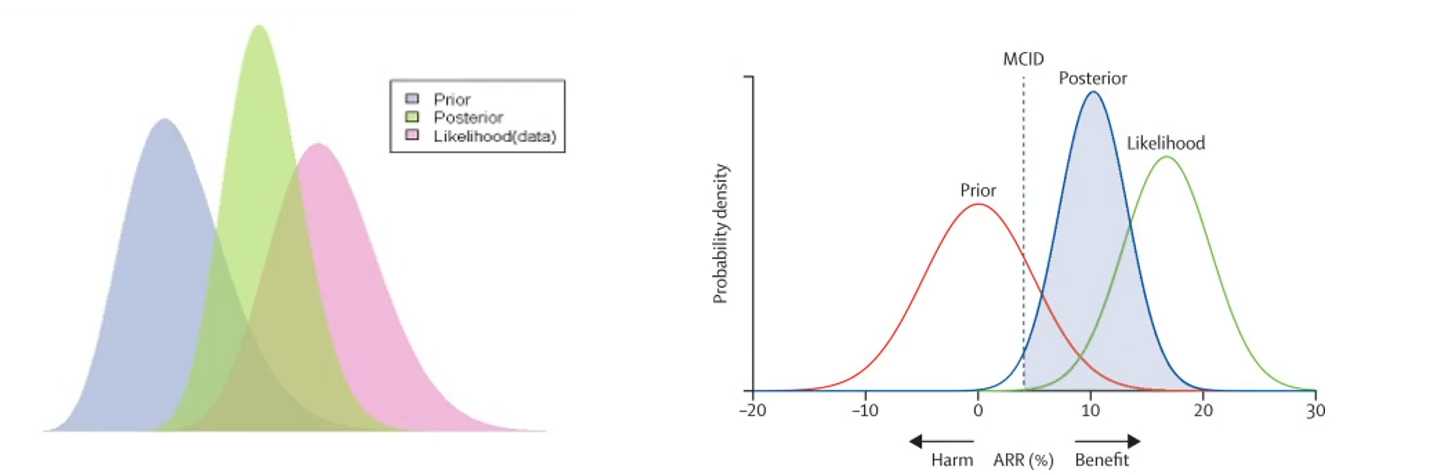
\includegraphics[width=\textwidth]{images/chapitre5/prior_likelihood_posterior.png}
	\end{center}
	\caption{La distribution à priori, à posteriori et celle de la fonction de vraisemblance.}
	\label{prior_likelihood_posterior}
\end{figure}

\subsubsection{Posterior distribution}
La probabilité postérieure est la probabilité qu'un événement se produise après que toutes les informations sur le système étudier aient été prises en compte. Elle est étroitement liée à la probabilité antérieure, qui est la probabilité qu'un événement se produise avant la pris en compte de nouvelles preuves. Elle est comme un ajustement sur la probabilité antérieure.

\begin{equation}
    \begin{split}
		Posterior \hspace{5pt} probability = prior \hspace{5pt} probability + new \hspace{5pt} evidence. \\
        Posterior \hspace{5pt} Distribution = Prior \hspace{5pt} Distribution + Likelihood \hspace{5pt} Function.
	\end{split}
	\label{posterior_probability_distribution}
\end{equation}

Par exemple, les données historiques suggèrent qu'environ 60\% des étudiants qui commencent l'université obtiendront leur diplôme dans les 6 ans. C'est la probabilité a priori. Cependant, ce chiffre est en réalité bien inférieur. Alors les preuves collecter peuvent suggérer que le chiffre réel est en fait plus proche de 50\% ; c'est la probabilité postérieure. \\
La distribution à posteriori est un moyen de résumer les connaissances ou les informations sur les quantités incertaines en analyse bayésienne. C'est une combinaison de la distribution a priori et de la fonction de vraisemblance, qui indique les informations contenues dans les données observées (les « nouvelles preuves »).

\subsubsection{Likelihood}
Habituellement lorsque l’on parle de distribution de probabilité, on suppose que nous connaissons les valeurs des paramètres. Aussi appelé fonction de vraisemblance (ou plus simplement vraisemblance), c’est une fonction des paramètres d'un modèle statistique calculée à partir de données observées \cite{fisher1922mathematical}. C’est-à-dire la probabilité d’observer les données sous un certain model. Par exemple, la probabilité des données sachant \(\displaystyle \theta \) en utilisant \ref{theoreme_bayes3}.
En inférence bayésienne, cette vraisemblance peut être interprète comme la densité de probabilité des données conditionnellement à une valeur des paramètres et comme une mesure de l'information apportée par les données sur la valeur des paramètres.

\subsubsection{Prior distribution}
La distribution à priori capture la connaissance ou l’information apriori. Elle permet de mettre en forme les connaissances ou les informations avant de faire l’expérimentation. Ces sont des distribution subjective sans tenir compte des données. \\
Ensuite Il y’a la probabilité des données, qui est défini par :

\begin{equation}
	Pr(data) = \int_{}^{}  \,L(data|\theta)Pr(\theta)d\theta .
	\label{probability_of_data}
\end{equation}

Le calcule d’une intégrale avec un seul paramètres (intégrale a une dimension) est possible mais lorsqu’il y’a plus d’un paramètre, cette dernière devient une intégrale multiple qui est difficile voire impossible à calculer. \\
L’approche Bayésienne d’aujourd’hui utilise des méthodes de simulation MCMC (chaine de Markov Monte Carlo) pour passer outre ce problème de calcule d’intégrale multiple. Nous verrons dans la section suivantes les chaines de Markov de Monte Carlo et leurs méthodes.

\subsubsection{Chaine de Markov Monte Carlo (MCMC)}
Malheureusement, dans la plupart des cas pratiques, il est impossible d’obtenir une solution analytique pour la distribution a posteriori. Le dénominateur sous la forme continue du théorème de Bayes consiste en une intégrale sur un espace potentiellement de grande dimension. L’un des moyens de résoudre ce problème est d’obtenir des échantillons de la distribution a posteriori. Parmi les approches les plus utilisées pour surmonter ces difficultés, on trouve les méthodes du Monte Carlo par chaînes de Markov et l’inférence variationnelle (dont nous n’évoquerons pas). Les méthodes de Monte Carlo par chaîne de Markov (MCMC) proposent des schémas pour dessiner,tirer (draw en anglais qui est présent dans les objets fit des résultats d’échantillonnages) une série d'échantillons corrélés qui convergent vers la distribution cible \cite{neal1993probabilistic}. \\

Les algorithmes MCMC consistent à simuler séquentiellement une seule chaîne de Markov dont la distribution limite est celle choisie (par example, le maximum de la fonction de vraisemblance fois une densité de probabilité a priori des paramètres). Plus précisément, une chaîne de Markov est une séquence de variables aléatoires telle que la valeur suivante ou état de la séquence dépend uniquement de l’état présent et non des états passés \cite{neal1993probabilistic}. Alors, une séquence de variables aléatoires est générée \(\displaystyle \widehat{q}_{0}, \widehat{q}_{1}, ... \)  telle que l’état suivant \(\displaystyle \widehat{q}_{t+1} \) avec \(\displaystyle t \geq 0  \) est distribué selon la probabilité de transition \(\displaystyle T(\widehat{q}_{t} \rightarrow \widehat{q}_{t+1}) \overset{def}{=} P(\widehat{q}_{t+1}|\widehat{q}_{t}) \) \cite{gbedo2017techniques} tout en visant la convergence de la chaine, c’est-à-dire que la chaîne est ergodique (stationnaire, irréductible et non périodique). \\

Une chaîne de Markov est définit par les valeurs initiales des distributions marginales des paramètres et la probabilité de transition entre deux états de l’espace des paramètres : \(\displaystyle T(\widehat{q} \rightarrow \widehat{q}^{\prime}) \), pour aller d’un état \(\displaystyle \widehat{q} \) à l’autre état \(\displaystyle \widehat{q}^{\prime} \). Les algorithmes MCMC sont généralement influencés lors de l’implémentation par le point de départ de la chaîne (ce qui conduit à une phase de « burn-in », comme l’illustre la figure \ref{mcmc_iterations}), par le choix de la probabilité de transition, le taux de convergence, l’acceptance de l’algorithme, etc. \\

\begin{figure}[H]
	\begin{center}
		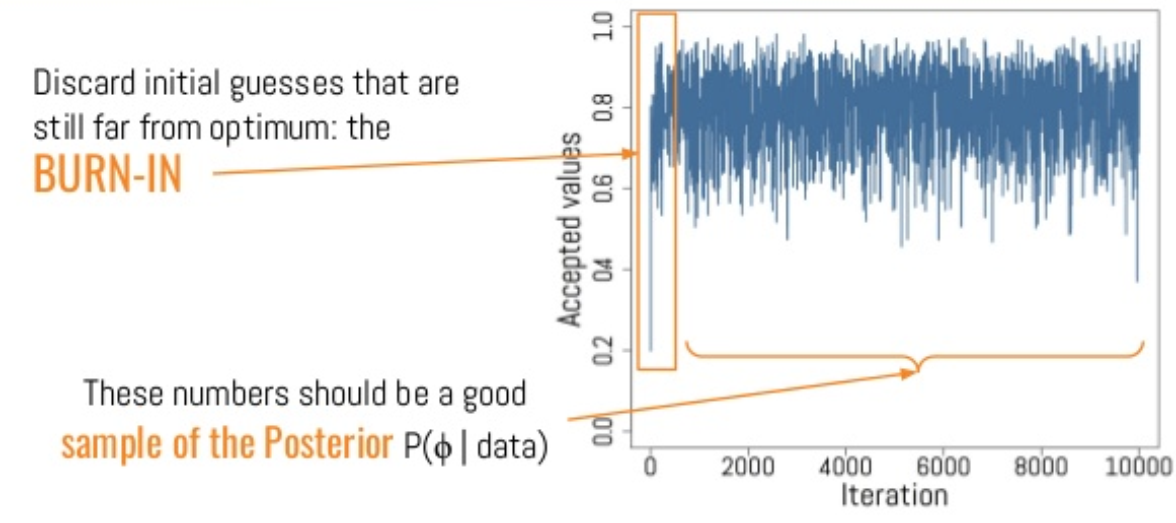
\includegraphics[width=\textwidth]{images/chapitre5/mcmc_iterations.png}
	\end{center}
	\caption{La phase « burn-in » d’une chaine de Markov et celle de la convergence de la chaine.}
	\label{mcmc_iterations}
\end{figure}

Les algorithmes de Monte Carlo à chaînes de Markov (MCMC) sont donc des outils informatiques standard pour analyser les modèles complexes bayésiens \cite{gelfand1990sampling} même si des fois des problème peuvent surgir dans leurs implémentations \cite{robert2020markov}. Parmi les méthodes MCMC, il y’a l’algorithme de Metropolis , l’algorithme de Metropolis–Hastings, échantillonnage de Gibbs, échantillonnage par tranches, Metropolis à tentatives multiples, Méthode de sur-relaxation l'hamiltonien Monte Carlo (HMC), No-U-Turn Sampler (NUTS), la méthode MCMC de Langevin et les méthodes basées sur le changement de dimension. Bien que notre travail ne soit pas centré sur les algorithmes MCMC, nous passerons en revue quelques définitions et théories qui justifient le fonctionnement des méthodes MCMC, et un bref résumé de quelque algorithmes MCMC. \\

\paragraph{Théorème de convergence des chaînes de Markov \cite{entezari2018bayesian} \cite{meyn2012markov} \cite{rosenthal2006first}}
Une chaîne de Markov à temps discret est définie par une séquence de variables aléatoires \(\displaystyle X_{0}, X_{2}, X_{3} ... \) qui peut prendre des valeurs possibles dans l'espace d'état \(\displaystyle X \) avec une distribution initiale définie pour \(\displaystyle X_{0}\) et des probabilités de transition définies comme :

\begin{equation}
	p(x,A) = P(X_{n+1} \in A | X_{n} = x), \hspace{1em} \forall A \subseteq X
\end{equation}
Où la propriété de Markov est :
\begin{equation}
	P(X_{n+1} \in A | X_{0},X_{1},...,X_{n}) = P(X_{n+1} \in A | X_{n})  \hspace{1em} \forall A \subseteq X
\end{equation}
Comme nous l’avons évoqué précédemment la probabilité que la chaîne passe à l'état suivant ne dépend que de l'état actuel et non des états précédents. \\
\textbf{\underline{Définition 1: }} Considérons une chaîne de Markov \(\displaystyle \left\{ X_{i} \right\} \) sur l'espace d'états \(\displaystyle X \) avec une probabilité de transition \(\displaystyle P(x,.) \). Soit \(\displaystyle \pi (.) \) une distribution de probabilité définie sur \(\displaystyle X \) . Alors \(\displaystyle \pi \) est une distribution stationnaire pour la chaîne de Markov  \(\displaystyle x,y \in X \) :

\begin{equation}
	\int_{x \in X}^{}  \,\pi(dx)P(x,dy) = \pi(dy)
\end{equation}

\noindent \textbf{\underline{Définition 2: }} Une chaîne de Markov est \(\displaystyle \phi \)-irréductible, s'il existe une mesure \(\displaystyle \sigma\)-finie non nulle sur \(\displaystyle X \) telle que :

\begin{equation}
	\begin{split}
	\forall A :  A \subseteq X \hspace{1em} avec \hspace{1em} \phi(A) > 0  \hspace{1em} \&  \hspace{1em} \forall x \in X \\
	\implies \exists \hspace{0.3em} n \in \mathbb{N} : P_{n}(x,A) > 0
	\end{split}
\end{equation}

\noindent \textbf{\underline{Définition 3: }} Une chaîne de Markov est apériodique, s'il n'y a pas de sous-ensembles disjoints non vides \(\displaystyle X_{1},...,X_{d} \subseteq X\) pour \(\displaystyle d \geq 2\) tel que \(\displaystyle P(x,X_{i+1}) = 1\) pour tout \(\displaystyle x \in X_{i} (1\leq i \leq d-1 ) \) et \(\displaystyle P(x,X_{1}) = 1 \) pour tout \(\displaystyle x \in X_{d}\). \\

\noindent \textbf{\underline{Théorème 1: }} Considérons une chaîne de Markov apériodique et \(\displaystyle \phi \)-irréductible définie sur un espace d'états \(\displaystyle X \) de distribution stationnaire \(\displaystyle \pi \). Pour \(\displaystyle \pi.a.e. \) \(\displaystyle x \in X \) :
\begin{equation}
	\lim_{x \to \infty} \left\lVert P^{n}(x,.) - \pi(.) \right\rVert = 0
\end{equation} 

\noindent Soit \(\displaystyle \lim_{x \to \infty} P^{n}(x,A) = \pi(A) \hspace{1em} \forall A \subseteq  X \) . \\
Dans la section suivante, nous décrirons quelques algorithmes MCMC les plus courants qui respectent l’aspect stationnaire, irréductible et non périodique des chaines de Markov.
\paragraph{Algorithme de Metropolis-Hastings}
L’algorithme de Metropolis-Hastings, proposé par METROPOLIS \cite{metropolis1953equation} et généralisé par HASTINGS \cite{hastings1970monte} est principalement utilisé comme moyen de simuler des observations à partir de distributions cibles. L'algorithme produit une chaîne de Markov dont la distribution limite des membres est la densité cible \(\displaystyle \pi(x) \) et qui s’itère en « sautant » de l’état actuel x de l’espace des paramètres à l’état suivant y avec une probabilité d’acceptation suivante :

\begin{equation}
	\alpha(x,y) = \min\Biggl( 1, \frac{\pi(y)q(y,x)}{\pi(x)q(x,y)} \Biggr)
\end{equation}

Où \(\displaystyle q(x,y) \) est la probabilité conditionnelle de proposer l'état \(\displaystyle y \) étant donné l'état \(\displaystyle x \). L'algorithme de Metropolis-Hastings est décrit dans l’algorithme \ref{m-c_algo}.

\begin{algorithm}
	\caption{Algorithme de Metropolis-Hastings \cite{entezari2018bayesian}}
	\label{m-c_algo}
	\begin{algorithmic}[1]
		\State Initial: value $X_{0}$, burn-in iterations $B$, number of samples $M$
		\State Output: $S_{1},...,S_{M}$ samples
		\For{$n$ in \{ $1,...,(B+M)$ \}}
			\State Draw $Y_{n}\sim Q(X_{n-1,.}) $, where $Q$ is the proposal distribution with probability density function q.
			\State Calculate $A_{n}$ = $\frac{\pi(Y_{n})q(Y_{n},Y_{n-1})}{\pi(X_{n-1})q(X_{n-1},Y_{n})}$
			\State Draw $U_{n} \sim $ Uniform[0,1]
			\If{$U_{n} < A_{n}$}
				\State $X_{n} = Y_{n}$ (« accept »)
			\Else
				\State $X_{n} = X_{n-1}$ (« reject »)
			\EndIf
		\EndFor
		\State \Return $S_{1} = X_{B+1},...,S_{M} = X_{B+M}$.
	\end{algorithmic}
\end{algorithm}

% \paragraph{Gibbs sampling}
\paragraph{Hamiltonian Monte Carlo}
L'hamiltonien Monte Carlo (HMC) est une méthode de Monte Carlo à chaîne de Markov (MCMC) capable de traiter des distributions cibles de grande dimension et qui utilise les dérivées de la fonction de densité échantillonnée pour générer des transitions efficaces couvrant la partie postérieure \cite{neal2011mcmc} \cite{betancourt2015hamiltonian}.Il utilise une simulation de dynamique hamiltonienne approximative basée sur une intégration numérique qui est ensuite corrigée en effectuant une étape d'acceptation Metropolis. Bien qu'il s'agisse d'un cas particulier d'échantillonneurs en temps continu, il peut être mis en œuvre en temps discret et est en fait à l'origine du succès du package Stan qui est utilisé dans la section implémentation \ref{irt_model_for_bayesian_inference}. L'hamiltonien Monte Carlo améliore l'efficacité en utilise le gradient du log postérieur pour diriger la chaîne de Markov vers les régions de densité postérieure plus élevée, où la plupart des échantillons sont prélevés, par conséquent, une chaîne HMC bien réglée acceptera les propositions à un taux beaucoup plus élevé que l'algorithme MH traditionnel \cite{gelman1997weak}. \\
Le processus repose sur une variable auxiliaire \(\displaystyle v \in \mathbb{R}^{d} \) qui augmente la distribution cible tout en échantillonnant à partir de \(\displaystyle \pi \) (une mesure cible de probabilité \(\displaystyle \pi \) sur \(\displaystyle \varTheta \subset \mathbb{R}_{d}\) par rapport à la mesure de Lebesgue, notée \(\displaystyle \pi(\theta) \infty \exp\{-U(\theta)\} \), où \(\displaystyle U \) est une fonction continûment dérivable appelée fonction de potentiel \cite{wu2018faster}. 
L’hamiltonien est défini par :
\begin{equation}
	H(\theta,v) = U(\theta) + \frac{1}{2}v^{T}M^{-1}v.
\end{equation}
\noindent Et HMC se base sur la dynamique hamiltonienne pour générer des propositions pour \(\displaystyle \theta \):
\begin{equation}
	\frac{d\theta}{dt} = \frac{\partial H}{\partial v} = M^{-1}v \hspace{0.5em} \text{et} \hspace{0.5em} \frac{dv}{dt} = - \frac{\partial H}{\partial \theta} = - \nabla U(\theta)
\end{equation}

\noindent L’algorithme HMC est :

\begin{algorithm}
	\caption{Algorithme de Monte Carlo hamiltonien \cite{wu2018faster}}
	\label{hmc_algo}
	\begin{algorithmic}[1]
		\State Initial: Starting point $\theta_{0}$ , step size $\epsilon $, number of leapfrog steps $L$, covariance matrix $M$, number of iterations $N$.
		\State Output: sample $\{ \theta_{0},...,\theta_{N}\}$ drawn from $\pi(\theta)$
		\For{$n \leftarrow 1$ to $N$}
			\State draw $v$ from $\mathcal{N}(\cdot|0,M)$ 
			\State compute $\theta^{\star},v^{\star} = Leapfrog(\theta_{n-1,v,\epsilon,L})$ compute
			\begin{equation}
				\rho = 1 \wedge \exp \{ H(\theta_{n-1},v) - H(\theta^{\star},-v^{\star})\}
			\end{equation}
			\State set
			\begin{equation}
				(\theta_{n},v_{n}) = \Biggl\{
				\begin{array}{ll}
					(\theta^{\star},-v^{\star}), \text{with probability} \rho \\
					(\theta_{n-1},v), \text{otherwise.}
				\end{array}
			\end{equation}
		\EndFor
		\State \Return $(\theta_{0},...,\theta_{N})$
		\Function{Leapfrog}{$\theta,v,\epsilon,L$}
			\State compute $(\theta_{0},v_{0}) = (\theta,v,- \epsilon / 2 \nabla U(\theta))$
			\For{$l \leftarrow 1$ to $L$}
				\State compute $\theta_{l} = \theta_{l-1} + \epsilon M^{-1}v_{l-1}$
				\State compute $v{l} = v_{l-1} -\epsilon \nabla U(\theta_{l})$
			\EndFor
			\State \Return $(\theta_{l},v_{l},+ \epsilon / 2 \nabla U(\theta_{l})$
		\EndFunction
	\end{algorithmic}
\end{algorithm}

\paragraph{No-U-Turn Sampler}
L’Hamiltonien Monte Carlo est un algorithme puissant, mais qui souffre de la nécessité d'ajuster le nombre d'étapes \(\displaystyle \mathcal{L}  \) par exemple en utilisant des heuristiques basées sur des statistiques d'autocorrélation à partir d'essais préliminaires coûteux \cite{neal2011mcmc}. Ce besoin de fixer le paramètre \(\displaystyle \mathcal{L}  \) est éliminé par l’algorithme No-U-Turn Sampler (NUTS). \\

Un échantillonneur MCMC qui utilise l’algorithme NUTS conserve la capacité de HMC à supprimer le comportement de marche aléatoire sans avoir besoin de définir le nombre \(\displaystyle \mathcal{L}  \) d'étapes de saut que l'algorithme prend pour générer une proposition. Le critère utilisé se base sur le produit scalaire entre \(\displaystyle \widetilde{r}  \) (la quantité de mouvement actuelle) et \(\displaystyle \widetilde{\theta} - \theta  \) (le vecteur de la position initiale à la position actuelle), qui est la dérivée par rapport au temps (dans le système hamiltonien) de la moitié de la distance au carré entre la position initiale \(\displaystyle \theta  \) et la position actuelle \(\displaystyle \widetilde{\theta}  \) \cite{hoffman2014no}:

\begin{equation}
	\frac{d}{dt} \frac{ (\widetilde{\theta} - \theta)^{T} (\widetilde{\theta} - \theta )}{2} = (\widetilde{\theta} - \theta)^{T} \frac{d}{dt} (\widetilde{\theta} - \theta) = (\widetilde{\theta} - \theta)^{T} \widetilde{r}.  
\end{equation}

\noindent Le pseudocode implémentant NUTS est fourni dans l'algorithme \ref{nuts_algo}. L'échantillonneur par défaut (NUTS) de Stan est plus efficace pour explorer le postérieur \cite{hoffman2011no}  \cite{hoffman2014no} et adapte automatiquement le nombre de pas de saut, éliminant le besoin de spécifier les paramètres de réglage par l'utilisateur.

\begin{algorithm}[H]
	\caption{No-U-Turn Sampler \cite{hoffman2011no}}
	\label{nuts_algo}
	\begin{algorithmic}[1]
		\State Resample $r \sim \mathcal{N} (0,I)$. ($I$ denote the identity matrix.)
		\State Resample $u \sim$ Uniform$(0,\exp\{\mathcal{L}(\theta^{t}) - \frac{1}{2}r^{T}r\})$. 
		\State Initalize $\theta^{-} = \theta^{t},\theta^{+} = \theta^{t}, r^{-} = r,r^{+} = r,j=0,\theta^{t+1} = \theta^{t},n=1,s=1.$
		\While{$s=1$}
			\State Chose a direction $v_{j} \sim$ Uniform$(\{-1,1\})$.
			\If{$v_{j} = -1$}
				\State $\{ \theta^{-},r^{-},-,-,\theta^{\prime},n^{\prime},s^{\prime} \} \leftarrow $ Recurse$(\theta^{-},r^{-},u,v_{j},j,\epsilon)$.
			\Else
				\State $\{ -,-,\theta^{+},r^{+},\theta^{\prime},n^{\prime},s^{\prime} \} \leftarrow $ Recurse$(\theta^{+},r^{+},u,v_{j},j,\epsilon)$.
			\EndIf
			\If{$s^{\prime} = 1$}
				\State With probability $\min\{ 1,\frac{n^{\prime}}{n} \}$, set $\theta^{t+1} \leftarrow \theta^{\prime} $.
			\EndIf
			\State $n \leftarrow n + n^{\prime}$.
			\State $s \leftarrow s^{\prime} \mathbb{I} \left[ (\theta^{+} - \theta^{-})^{T} r^{-} \geq 0  \right] \mathbb{I} \left[ (\theta^{+} - \theta^{-})^{T} r^{+} \geq 0  \right]  $.
			\State $j \leftarrow j+1$.
		\EndWhile
		\Function{Recurse}{$\theta,r,u,v,j,\epsilon$}
			\If{$j=0$}
				\State Base case take one leapfrog step in the direction v.
				\State $r^{\prime} \leftarrow \frac{v \epsilon}{2} \nabla_{\theta} \mathcal{L} (\theta)$.
				\State $\theta^{\prime} \leftarrow v \epsilon r^{\prime}$.
				\State $r^{\prime} \leftarrow \frac{v \epsilon}{2} \nabla_{\theta} \mathcal{L} (\theta^{\prime})$.
				\State $n^{\prime} \leftarrow \mathbb{I} \left[ u \leq \exp \{ \mathcal{L} (\theta^{\prime}) - \frac{1}{2} r^{\prime T} r^{\prime}\} \right] $.
				\State $s^{\prime} \leftarrow \mathbb{I} \left[ \mathcal{L} (\theta^{\prime}) - \frac{1}{2} r^{\prime T} r^{\prime} > u - \Delta_{\max}  \right] $
				\State \Return $\{ \theta^{\prime},r^{\prime},\theta^{\prime},r^{\prime},\theta^{\prime},n^{\prime},s^{\prime} \}$.
			\Else
				\State Recursion implicitly build the left and right subtrees.
				\State $\{ \theta^{-},r^{-},\theta^{+},r^{+},\theta^{\prime},n^{\prime},s^{\prime} \} \leftarrow $ Recurse$(\theta,r,u,v,j-1,\epsilon)$.
				\If{$s^{\prime} = 1$}
					\If{$v = -1$}
						\State $\{ \theta^{-},r^{-},-,-,\theta^{\prime \prime},n^{\prime \prime},s^{\prime \prime} \} \leftarrow $ Recurse$(\theta^{-},r^{-},u,v,j-1,\epsilon)$.
					\Else
						\State $\{ -,-,\theta^{+},r^{+},\theta^{\prime \prime},n^{\prime \prime},s^{\prime \prime} \} \leftarrow $ Recurse$(\theta^{+},r^{+},u,v,j-1,\epsilon)$.
					\EndIf
					\State With probability $\frac{n^{\prime \prime}}{n^{\prime} + n^{\prime \prime}}$, set $\theta^{\prime} \leftarrow \theta^{\prime \prime}$.
					\State $s \leftarrow s^{\prime \prime} \mathbb{I} \left[ (\theta^{+} - \theta^{-})^{T} r^{-} \geq 0  \right] \mathbb{I} \left[ (\theta^{+} - \theta^{-})^{T} r^{+} \geq 0  \right]  $. 
				\EndIf
				\State \Return $\{ \theta^{-},r^{-},\theta^{+},r^{+},\theta^{\prime},n^{\prime} + n^{\prime \prime},s^{\prime} \}$.
			\EndIf
		\EndFunction
	\end{algorithmic}
\end{algorithm}

% Malheureusement, dans la plupart des cas pratiques, il est impossible d'obtenir une solution analytique pour la distribution a posteriori. Le dénominateur sous la forme continue du théorème de Bayes consiste en une intégrale sur un espace potentiellement de grande dimension. L'un des moyens de résoudre ce problème est d'obtenir des échantillons de la distribution a posteriori. Ces échantillons sont distribués selon la distribution a posteriori.  \\
% Habituellement, les méthodes dites de Markov Chain Monte Carlo (MCMC) sont utilisées pour obtenir des échantillons à partir d'une distribution. Ces méthodes partent des valeurs initiales des paramètres. Ensuite, de nouvelles valeurs sont proposées et acceptées selon certaines fonctions de proposition et d'acceptation. Ce processus de proposition et d'acceptation est répété plusieurs fois pour créer un grand nombre d'échantillons. Différentes méthodes diffèrent principalement dans leurs implémentations des fonctions de proposition et d'acceptation. \\
% Les méthodes MCMC peuvent nécessiter un certain post-traitement des échantillons obtenus - par exemple, il peut être nécessaire d'ignorer les premiers (souvent des centaines ou des milliers) échantillons, car « ils ont été collectés loin des valeurs des paramètres pertinents » par exemple la figure ci-dessous. De plus, les échantillons sont généralement corrélés et donc souvent, seul un nième échantillon (après le retrait des échantillons initiaux) est retenu. De plus, les méthodes peuvent échouer (pour donner des échantillons représentatifs de la distribution). Il existe des moyens de diagnostiquer cela, par exemple en créant plusieurs « chaînes d'échantillonnage » (et en comparant leurs résultats). \\
%Plusieurs méthodes sont utilisées pour construire ces chaines comme : Metropolis-Hastings, Gibbs sampler, Metropolis-within-Gibbs, HMC etc.

\subsection{Méthodes de vérifications et de comparaison de modèles}
Les méthodes de vérifications de modèles sont différentes des méthodes de comparaisons du fait qu’elles permettent d'examiner si un modèle capture les caractéristiques importantes d'un ensemble de données, tandis que les méthodes de comparaisons répondent à la question de savoir quel modèle parmi un groupe de modèles candidats est le meilleur. \\
La théorie des réponses aux items (TRI) dans le cadre bayésien comme tout autres méthodes permettent une analyse plus approfondie en utilisant des distributions postérieures du modèle. En général, certaines techniques populaires de vérification de modèle bayésien qui ont été appliquées à l'IRT comprennent l'analyse résiduelle bayésienne, les vérifications prédictives préalables et les vérifications prédictives postérieures, et les méthodes de comparaison de modèles bayésiens incluent le critère d'information sur la déviance DIC \cite{spiegelhalter2003bayesian}, le facteur de Bayes \cite{kass1995bayes} et la probabilité de validation croisée et le facteur de Bayes partiel \cite{o1995fractional}. \\
Pour faire de la sélection de modèle (en comparant plusieurs modèles) il faut vérifier s’il y’a un effet des valeurs des paramètres sur la variable cible (par exemple sur la réussite ou pas à un item). \\
Dans le cadre fréquentiste, l’idée est de pénalisé les modèles qui ont trop de paramètres. Pour le faire il y’a \(\displaystyle AIC \)  :

\begin{equation}
	AIC = -2 \log (L(\widehat{\theta_{1}},...,\widehat{\theta_{k}} )) + 2K.
	\label{aic_formula}
\end{equation}

Avec \(\displaystyle L \) la vraisemblance et \(\displaystyle k \) le nombre de paramètres \(\displaystyle \theta \), et \\
\(\displaystyle -2 \log (L(\widehat{\theta_{1}},...,\widehat{\theta_{k}} )) \) est la déviance qui mesure la qualité de l’ajustement du model de donnée. Plus il y’a de paramètres plus cette quantité est petite et mieux le model est ajuster aux données. \\
\(\displaystyle 2k \) : c’est la pénalité, plus il y’a des paramètres plus cette quantité augmente. Cette pénalité est un équilibre entre l’ajustement du model des données et la complexité du model qui est capturer par le nombre de paramètres. \\ \\

\noindent En bayésien, le critère d'information WAIC (Watanabe Akaike Information Criteria) et la validation croisée LOO (leave-one-out cross-validation) sont considéré comme des méthodes de sélection de modèles entièrement bayésiennes en raison de leur utilisation de l'ensemble a posteriori distribution autre que les estimations ponctuelles. \\

\noindent WAIC \cite{watanabe2010asymptotic} est une méthode de sélection de modèle entièrement bayésienne basé sur un critère d'information et est considéré comme une version améliorée de DIC, définit comme suit :
%\noindent En bayésien il y’a WAIC (Watanabe Akaike Information Criteria) définit par :

\begin{equation}
	WAIC = -2\sum_{i=1}^{n} \log E\left[ p(y_{i}|\theta) \right] + 2p_{WAIC}
	\label{waic_formula}
\end{equation}

Où \(\displaystyle E\left[ p(y_{i}|\theta) \right] \) est la moyenne a posteriori de la vraisemblance de la ième observation.
\(\displaystyle Pwaic \)  est le nombre effectif de paramètres calculés en utilisant la variance postérieure de la vraisemblance.
La valeur de waic est la somme entre la deviance + le nombre de paramètre pwaic. \\

\noindent Une autre méthode de comparaison de modèles entièrement bayésienne est la validation croisée LOO \cite{geisser1979predictive} définit : \\

\begin{equation}
	LOO = -2\sum_{i=1}^{n} \log \int \,p(y_{i}|\theta)p_{post(-i)}(\theta)d\theta.
	\label{loo_formula}
\end{equation}
 Où \(\displaystyle p_{post(-i)}(\theta) \) est la distribution postérieure basée sur les données moins le point de données \(\displaystyle i \).
\section{La théorie des réponses aux items}
La théorie des réponses aux items (TRI) aussi appelé théorie des traits latents, théorie du vrai score fort ou théorie moderne des tests mentaux est un paradigme pour la conception, l’analyse et la notation des test et des questionnaires \cite{fisher1922mathematical}. TRI intervient dans la mesure ou la théorie classique n’apporte pas toujours des réponses satisfaisantes. Par exemple un item jugé facile ou difficile peut ne plus l’être dans un échantillon différent qu’il appartenait.

Dans cette situation, la théorie des réponses aux items tente de produire des propriétés de l’item qui soit indépendante d’un groupe particulier d’individus. En d'autres termes, il s'agit de parvenir à l'élaboration d'instruments de mesure dont les caractéristiques ne soient pas excessivement influencées par tel ou tel autre groupe de référence : ce qui, d'une certaine manière, conduit à définir des échelles qualifiées parfois d'"absolues" \cite{xcv_wiki}. La première tentative de développement de ce type d’échelle remontre au début des années 1950 (échelle de Guttman). Initialement, ils reposaient sur un modèle totalement déterministe qui a ensuite été remplacé par un modèle plus réaliste de type probabiliste (modèle de Rasch). Ces modèles reposent sur l’hypothèse selon laquelle la réponse d’un individu a un item est déterminée ou peut être expliquer par deux facteurs qui sont :

\begin{itemize}
	\item D’une part, certains attributs du sujet (sa compétence par exemple), qui, n'étant pas directement accessibles à l'observation et à la mesure, sont généralement qualifiés de traits latents \cite{xcv_wiki} ;
	\item D’autre part, les propriétés de l'item lui-même, notamment, sa difficulté, son pouvoir de discrimination, sans oublier le rôle que la "chance" (réponses "au hasard") peut jouer dans certains cas \cite{xcv_wiki}.
\end{itemize}

Sur le plan technique et mathématique, la théorie des réponses aux items utilise des modèles à un, deux ou trois paramètre(s), qui établissent la relation fondamentale entre le trait latent de l'individu (son niveau de compétence par exemple) et la probabilité pour cet individu de réussir un item donné. Cette relation est formalisée par une fonction (appelée fonction caractéristique de l'item), et peut être représentée géométriquement par une courbe (la courbe caractéristique de l'item). La forme la plus simple de cette fonction est celle qui repose sur le modèle de Rasch \cite{xcv_wiki}.\\
L'objectif de la méthode est double, il s'agit, d'une part, d'estimer les propriétés métriques des items (calcul des paramètres dits de difficulté, de discrimination et, éventuellement, de pseudo-chance) et, d'autre part, d'estimer le niveau de l'individu par rapport au trait latent considéré. Par ailleurs, ces estimations sont supposées indépendantes des échantillons particuliers (d'individus d'une part et d'items de l'autre) à partir desquels l'étude est réalisée \cite{xcv_wiki}.
\subsection{IRT dans la recherche organisationnelle}
Les modèles de la théorie des réponses aux items (TRI) présentent plusieurs avantages pour la recherche organisationnelle. L’un des avantages méthodologiques de l’IRT est la détection des réponses aberrante parmi d’autre avantage comme la construction et l’évaluation des échelles et l’examen des biais de mesure. Le tableau \ref{irt_application} présente un résumé de ces applications ainsi que quelques avantages par rapport aux approches alternatives.
\begin{table}[H]
	\centering
	\addtolength{\leftskip} {-4cm}
	\addtolength{\rightskip}{-4.5cm}
	\begin{tabular}{|m{4cm}|m{6cm}|m{6cm}|}
	\hline
	\textbf{Problèmes méthodologiques} & \textbf{Applications de l'IRT} & \textbf{Avantages de l'IRT par rapport aux méthodes alternatives}  \\ \hline
	Construction et évaluation de l'échelle 
	 & 
	\begin{itemize}[leftmargin=*]
	    \item Peut être utilisé pour raccourcir une échelle ou examiner la qualité des échelles existantes
	    \item Peut être utilisé pour développer d'autres types d'évaluations.
	\end{itemize}
	& 
	\begin{itemize}[leftmargin=*]
		\item Contrairement au CTT, les paramètres des éléments IRT sont invariants d'un échantillon à l'autre.
		\item IRT peut être utilisé pour créer des tests adaptatifs, mais pas CTT.
		\item Bien que les méthodes CTT soient cohérentes avec les modèles de dominance, l'IRT peut être utilisé pour créer des mesures ponctuelles idéales.
	\end{itemize} \\ \hline
	% & \cite{borman2001examination} \cite{carter2011using} \cite{chernyshenko2007constructing} \cite{roznowski1989examination} \cite{tay2009fitting}

	Identifier l'élément (l'item) et tester le biais &
	\begin{itemize}[leftmargin=*]
	    \item Peut différencier les différences moyennes observées du biais
	    \item Peut détecter les DIF et DTF compensatoires
	    \item Peut examiner les différences au niveau des options
	\end{itemize}
	&
	\begin{itemize}[leftmargin=*]
	    \item La comparaison des différences moyennes avec le CTT confond le biais avec de vraies différences dans le trait latent.
	    \item Les modalités d'examen du DTF sont plus développées qu'en CFA.
	\end{itemize}\\ \hline
	% & \cite{chan1999shelf} \cite{nye2010never} \cite{raju2002measurement} \cite{stark2004examining} \cite{tay2015overview} 

	Détection des réponses aberrantes &
	\begin{itemize}[leftmargin=*]
	    \item Peut être utilisé pour détecter différents types de réponses aberrantes telles que IER, falsification et réponse faussement faible.
	\end{itemize}
	&
	\begin{itemize}[leftmargin=*]
	    \item Les méthodes IRT peuvent détecter plusieurs types de réponses aberrantes tandis que d'autres méthodes ne peuvent détecter que des réponses imprudentes.
	    \item Les méthodes IRT sont souvent plus efficaces pour détecter les réponses aberrantes que les méthodes traditionnelles de réponse à l'effort insuffisant (IER).
	\end{itemize}\\ \hline
	% & \cite{stark2001effects} \cite{drasgow1996optimal} \cite{zickar1999modeling} \cite{zickar2004uncovering} 
    \end{tabular}
	\caption{Résumé des applications de l'IRT \cite{nye2020advancing}.}
	\label{irt_application}
\end{table}


\subsection{Les Modèles IRT}
On distingue deux familles de modèle IRT : les modèles unidimensionnels qui nécessitent une seule dimension de trait et les modèles multidimensionnels qui sont supposées provenir de plusieurs traits. Cependant, en raison de la complexité considérablement accrue, la majorité des recherches et des applications IRT utilisent un modèle unidimensionnel. \\

Les modèles IRT se distingue par le nombre de paramètre qu’il utilise. Le modèle à paramètre unique (1PL) suppose tous les éléments qui correspondent au modèle ont la même difficulté, de sorte que ces éléments sont décrits par un seul paramètre. C’est le cas du modèle de Rasch. Le modèle dit à deux paramètre (2PL) fait appel au paramètre de difficulté et de discrimination par exemple le modèle de Birnbaum. Par contre le modèle a trois paramètres (3PL) est celui qui cherche à estimer en plus le paramètre de difficulté et de discrimination, la pseudo chance. \\
Il en résulte des modèles à un paramètre ayant la propriété d'objectivité spécifique, ce qui signifie que le rang de la difficulté de l'item est le même pour tous les répondants indépendamment de la capacité, et que le rang de la capacité de la personne est le même pour les items indépendamment de la difficulté. Ainsi, les modèles à 1 paramètre (comme ceux de Rasch) sont indépendants de l'échantillon, une propriété qui n'est pas valable pour les modèles à deux et trois paramètres \cite{fisher1922mathematical}. \\
Le modèle général de Birnbaum, auquel le modèle de Rasch se rattache est plus complexe car il admet des courbes d’allures différentes pour chacun des items et suppose donc d’estimer plus d’un paramètre par item puisqu’il tient également compte du pouvoir discriminant de chacun d’eux. Le modèle proposé par Lazarsfeld est en quelque sorte une simplification du modèle général de Birnbaum puisqu’il postule des distributions linéaires de pentes variables \cite{yvonnick_2019}. \\
Il existe aussi d’autre modèles IRT qui sont résumé dans le tableau \ref{irt_modeles}.

\begin{table}[H]
	\centering
	\addtolength{\leftskip} {-4cm}
	\addtolength{\rightskip}{-4.5cm}
	\begin{tabular}{|m{4cm}|m{6cm}|m{6cm}|}
	\hline
	\textbf{Modèle IRT} & \textbf{Description} & \textbf{Application} \\ \hline
	% Modèle logistique à un paramètre (One-parameter logistic model \textbf{1PL}) & & \\ \hline
	% Modèle logistique à deux paramètres (Two-parameter logistic model \textbf{2PL}) & Suit un processus de réponse de dominance et suppose que tous les items varient en fonction de la discrimination \(\displaystyle (a_{i})\) et de la difficulté \(\displaystyle (b_{i})\). & Utilisé pour les éléments dichotomiques (par exemple, oui/non ou correcte/incorrecte) pour lesquels il est peu probable de deviner (par exemple, les questions ouvertes avec de nombreuses réponses possibles). \\ \hline
	% Modèle logistique à trois paramètres (Three-parameter logistic model \textbf{3PL}) & Suit un processus de réponse de dominance et suppose que tous les items varient en fonction de la discrimination \(\displaystyle (a_{i})\), de la difficulté \(\displaystyle (b_{i})\) et de la pseudo-chance \(\displaystyle (c_{i})\). & Utilisé pour les éléments dichotomiques pour lesquels des devinettes sont susceptibles de se produire (par exemple, éléments avec une bonne ou une mauvaise réponse ou des options de réponse oui/non).\\ \hline
	Modèle logistique multidimensionnel à deux paramètres (Multidimensional two-parameter logistic model \textbf{M2PL}) & Suit un processus de réponse de dominance et suppose que tous les items varient sur un vecteur de paramètres de discrimination \(\displaystyle (a_{i} = a_{1},...,a_{m} )\) et de difficulté \(\displaystyle (b_{i})\). & Utilisé pour les éléments dichotomiques où il est peu probable de deviner. Peut être utilisé lorsque les données sont multidimensionnelles.\\ \hline
	Modèle de réponse graduée (Graded response model \textbf{GRM}) & Suit un processus de réponse de dominance et suppose que tous les items varient en fonction de la discrimination \(\displaystyle (a_{i})\) et que chaque option de réponse varie en fonction de la difficulté \(\displaystyle (b_{ik})\). En d'autres termes, chaque élément aura un paramètre a et \(\displaystyle C - 1 \) paramètres \(\displaystyle b \), où \(\displaystyle C \) est le nombre total d'options de réponse. & Utilisé pour les éléments polytomiques avec trois options de réponse ou plus.\\ \hline
	Modèle de réponse graduée multidimensionnelle (Multidimensional graded response model \textbf{MGRM}) &Suit un processus de réponse de dominance et suppose que tous les items varient sur un vecteur de paramètres de discrimination \(\displaystyle (a_{i} = a_{1},...,a_{m} )\) et chaque option de réponse varie en fonction de la difficulté \(\displaystyle (b_{ik})\). Chaque élément aura un vecteur d'un paramètre pour chaque facteur latent et des paramètres \(\displaystyle C - 1 \) \(\displaystyle b \), où \(\displaystyle C \) est le nombre total d'options de réponse. & Utilisé pour les éléments polytomiques avec trois options de réponse ou plus. Peut être utilisé lorsque les données sont multidimensionnelles.\\ \hline
	Modèle de dépliage gradué généralisé (Generalized graded unfolding model \textbf{GGUM}) & Suit un processus de réponse ponctuelle idéal et suppose que tous les éléments varient en fonction de la discrimination \(\displaystyle (a_{i})\), de l'emplacement de l'élément \(\displaystyle (\delta_{i})\) et des seuils \(\displaystyle (\tau_{i1})\). & Peut être utilisé pour les éléments ponctuels idéaux dichotomiques ou polytomiques. \\ \hline
	\end{tabular}
	\caption{Résumé des quelques modèles IRT \cite{nye2020advancing}.}
	\label{irt_modeles}
\end{table}

\begin{figure}[H]
	\begin{center}
		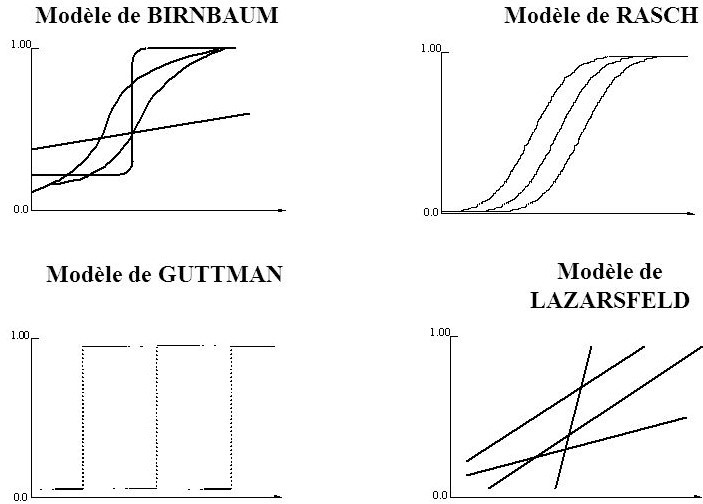
\includegraphics[width=\textwidth]{images/chapitre5/irt_models.jpg}
	\end{center}
	\caption{Les modèles IRT.}
	\label{irt_models}
\end{figure}

\subsubsection{Le modèle Rasch}
La structure cumulative ou d’emboitement du scalogramme de Guttman rend les analyses exploratoires traditionnelles mal appropriées (AFC par exemple) . Dans cette situation Rasch a proposé en 1960 une représentation numérique des niveaux de compétences de sujets et de difficulté d’items. Le modèle de Rasch qui est le modèle a un paramètre (1PL), est considéré comme l’approche la plus simple pour modéliser la relation entre le trait latent et la probabilité de réussir correctement un item. Dans le modèle de Rasch chaque sujet est caractérisé par un niveau \(\displaystyle \theta i \) d’aptitude \(\displaystyle (i=1,...,N) \) sur un continuum numérique latent.
Le modèle de Rasch cherche a donné du sens non pas seulement au classement des sujets par compétences, non pas seulement au classement des items par difficultés mais le modèle cherche à donner du sens dans le fait que les coordonnées d’un sujet peuvent être directement et numériquement comparer à la difficulté d’un item pour qu’on puisse dire par exemple que ce sujet à la compétence nécessaire pour pouvoir résoudre l’item de tel difficulté. Donc ça devient possible de les comparer directement à partir du moment où on les projette sur une seule et même dimension (cet \(\displaystyle \theta i \) de sujet et \(\displaystyle \beta i \) d’item). La probabilité de réussir l’item est une fonction croissante de la différence \(\displaystyle \theta i - \beta j\) \cite{yvonnick_2019}.
Rasch propose la fonction logistique suivant \cite{mislevy1994evidence}:




\begin{equation}
    \begin{split}
		P(x_{1},...,x_{n} | \theta, \beta_{1},...,\beta_{n}) = \prod_{j=1}^{n} P(x_{j}| \theta, \beta_{j}), \hspace{10pt} avec, \\
		P(x_{j}| \theta, \beta_{j}) = \frac{\exp \left[\theta - \beta_{j} \right]  }{1+ \exp \left[ \theta - \beta_{j} \right] }
	\end{split}
	\label{posterior_probability_distribution}
\end{equation}

\begin{figure}[H]
	\begin{center}
		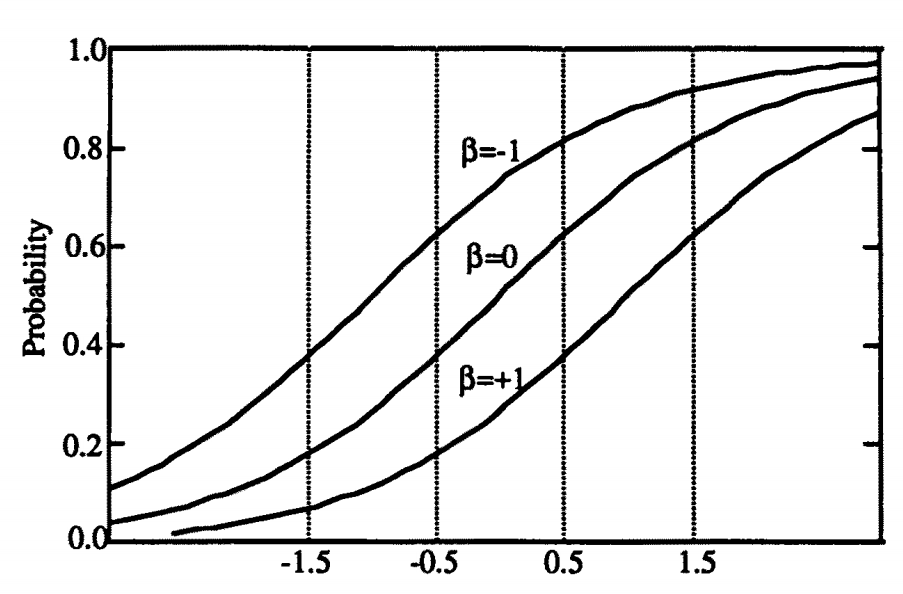
\includegraphics[width=\textwidth]{images/chapitre5/parameters_probability.png}
	\end{center}
	\caption{Probabilité de bonne réponse, conditionnelle à thêta, pour les items avec bêta = -1,0 et 1.}
	\label{parameters_probability}
\end{figure}
Où \(\displaystyle x_{j} \)  est la réponse à l'élément \(\displaystyle j \) (1 pour correcte, 0 pour incorrecte). La figure \ref{parameters_probability} montre les probabilités de réponse correcte à trois éléments, avec les paramètres de difficulté - 1 , 0 et + 1, en fonction de \(\displaystyle \theta \). Des valeurs faibles de \(\displaystyle \theta \) indiquent des chances plus faibles de réponse correcte et des valeurs élevées indiquent des chances plus élevées \cite{mislevy1994evidence}.

\subsubsection{Modèle logistique à deux paramètres}
Le modèle de Rasch suppose que tous les items ont la même forme, mais cette hypothèse pourrait ne pas être raisonnable. Pour éviter cette hypothèse, le modèle logistique a deux paramètres inclut le paramètre de discrimination des items. Le paramètre de discrimination est une mesure de la capacité différentielle d'un élément. Une valeur élevée du paramètre de discrimination suggère un élément qui a une grande capacité à différencier les sujets. En pratique, une valeur élevée du paramètre de discrimination signifie que la probabilité d'une réponse correcte augmente plus rapidement à mesure que la capacité (trait latent) augmente. La probabilité d'une réponse correcte est donnée par la formule suivante. \\

\begin{equation}
    P_{i}(\theta_{j} | X=1) = \frac{\exp \left[ \alpha_{i}(\theta_{j}-\beta_{i}) \right]  }{1+ \exp \left[ \alpha_{i}(\theta_{j}-\beta_{i}) \right]  } 
	\label{2pl_model_equation}
\end{equation}

\subsubsection{Modèle logistique à trois paramètres}
Le modèle logistique a trois paramètres (3PL) a été proposé par Birnbaum en 1968 incluant le paramètre de pseudo-chance dans le modèle. Le modèle 3PL spécifie la probabilité de réponse correcte sur le ième élément à l'aide de l'équation suivante. \\

\begin{equation}
    P_{i}(\theta_{j}) = c_{i} +  \frac{1 - c_{i}}{1+ \exp \left[ -\alpha_{i}(\theta_{j}-\beta_{i}) \right]  } 
	\label{3pl_model_equation}
\end{equation}

\subsection{Estimation des paramètres}
L'estimation des paramètres surtout dans un cadre bayésien est effectuée à l’aide des méthodes Markov Chain Monte Carlo implémentée dans plusieurs logiciels comme OpenBUGS \cite{lunn2009bugs}, JAGS \cite{plummer2003jags}, Stan \cite{stan} etc. Les prior les plus utilisé dans les modèles pour l'estimation MCMC des paramètres du modèle sont : \\

\begin{equation}
	\begin{split}
		\theta_{j} \sim Normal(0,1), \hspace{1em} j = 1,...N \hspace{1em} ou \\
		\theta_{j} \sim Uniform(-4,4), \hspace{1em} j = 1,...N  \\
	\end{split}	
	\label{prior_subjects}
\end{equation}
\noindent Et,
\begin{equation}
	\begin{split}
		\beta_{i} \sim Normal(0,1), \hspace{1em} i = 1,...n \\
		\alpha_{i} \sim Normal(0,1), \hspace{0.5em} et \hspace{0.5em} \alpha_{i} > 0 , \hspace{0.1em} i = 1,...n \\
		c_{i} \sim Beta(5,17) \hspace{0.5em}  et \hspace{0.5em} 0<c_{i}<0.3, \hspace{1em} i = 1,...n 
	\end{split}	
	\label{prior_items}
\end{equation}

% \subsection{Analyses de récupération d'items}

\section{Un ajustement bayésien des réponses aux items avec Stan}
Stan est une plate-forme pour la modélisation statistique, l'analyse de données et la prédiction dans les sciences sociales, biologiques et physiques, l'ingénierie et les affaires.
Il permet de spécifier les fonctions de densité de log afin d’obtenir :

\begin{itemize}
	\item Inférence statistique bayésienne complète avec échantillonnage MCMC (NUTS, HMC)
	\item Inférence bayésienne approximative avec inférence variationnelle (ADVI)
	\item Estimation du maximum de vraisemblance pénalisée avec optimisation (L-BFGS)
\end{itemize}

\noindent La bibliothèque mathématique de Stan fournit des fonctions de probabilité différentiables et une algèbre linéaire (C++ autodiff).
Stan peut être utilisé avec les langages d'analyse de données les plus populaires (R, Python, shell, MATLAB, Julia, Stata) et fonctionne sur toutes les principales plates-formes (Linux, Mac, Windows) \cite{stan}.

\subsection{IRT avec Stan}
La théorie de l'item-réponse (TRI) modélise la situation dans laquelle un certain nombre d'étudiants répondent chacun à une ou plusieurs questions d'un groupe de questions de test. Le modèle est basé sur des paramètres pour la capacité des étudiants, la difficulté des questions, et dans des modèles plus articulés, le caractère discriminant des questions et la probabilité de deviner correctement \cite{data_analysis_irt}.

\subsubsection{Déclaration des données}
Les données fournies pour un modèle IRT peuvent être déclarées comme suit pour tenir compte du fait que tous les étudiants ne sont pas tenus de répondre à toutes les questions. Ces données sont dans le bloc « data » où les informations pertinentes sur les données et les données elles-mêmes sont spécifier.


\begin{lstlisting}[language=Stan,basicstyle=\scriptsize, frame=l,framesep=4.5mm,framexleftmargin=2.5mm,tabsize=2,numbers=left,fillcolor=\color{blueforest!70},rulecolor=\color{blueforest},numberstyle=\normalfont\tiny\color{white}]
data {
	// numbers of things
	int<lower=1> N;  // number of observations
	int<lower=1> I;  // items,  number of questions  
	int<lower=1> S;  // subjects,  number of users 
	// data
	int<lower=1,upper=I> item[N];
	int<lower=1,upper=S> subject[N];
	int<lower=0,upper=1> grade[N];
	// data for posterior prediction using new data also used for Cross-validation
	int<lower=1> N_new;
	int<lower=1,upper=I> item_new[N_new];
	int<lower=1,upper=S> subject_new[N_new];
}
\end{lstlisting}
Dans cette déclaration il y’a \(\displaystyle N \) un entier positif qui est le nombre d’observation, où pour toute valeurs \(\displaystyle n \) de \(\displaystyle 1 \) à \(\displaystyle N \) \(\displaystyle grade[n] \) est la réponse obtenue par l’étudiant \(\displaystyle subject[n] \) à la question \(\displaystyle item[n] \).

\subsubsection{Les paramètres du model de Rasch, 2PL et 3PL}
Les paramètres des modèles IRT sont :

\begin{lstlisting}[language=Stan,basicstyle=\scriptsize, frame=l,framesep=4.5mm,framexleftmargin=2.5mm,tabsize=2,numbers=left,fillcolor=\color{blueforest!70},rulecolor=\color{blueforest},numberstyle=\normalfont\tiny\color{white}]
parameters {
	// parameters
	real ability[S];             //  alpha: ability of student
	real difficulty[I];          //  beta: difficulty of question
	real delta;                   // mean student ability
	// end for Rasch model
	vector<lower=0>[I] discrimination;      // discrimination of question
	// end for 2PL
	vector<lower=0,upper=1>[I] guessing;    //
	// end for 3PL
}
\end{lstlisting}
Le paramètre  \(\displaystyle ability_{i} \) est le coefficient de capacité de l'élève \(\displaystyle S_{i} \) , \(\displaystyle difficulty_{j} \) le coefficient de difficulté de la question \(\displaystyle I_{j} \), \(\displaystyle discrimination_{i} \) qui modélise à quel point l’item k est discriminant et \(\displaystyle guessing_{i} \) le paramètre de pseudo hasard. La paramétrisation non standard utilisée comprend également un terme d'interception delta, qui représente la réponse moyenne de l'étudiant à la question moyenne \cite{data_analysis_irt}.

\subsubsection{Le model de Rasch, 2PL et 3PL}
Le model de Rasch:
\begin{lstlisting}[language=Stan,basicstyle=\scriptsize, frame=l,framesep=4.5mm,framexleftmargin=2.5mm,tabsize=2,numbers=left,fillcolor=\color{blueforest!70},rulecolor=\color{blueforest},numberstyle=\normalfont\tiny\color{white}]
model {
	ability ~ normal(0,1);         
	difficulty ~ normal(0,1);   
	delta ~ normal(0.75,1);
	for(n in 1:N)
		grade[n] ~ bernoulli_logit(ability[subject[n]] - difficulty[item[n]] + delta);
}
\end{lstlisting}
Modèle logistique à deux paramètres:
\begin{lstlisting}[language=Stan,basicstyle=\scriptsize, frame=l,framesep=4.5mm,framexleftmargin=2.5mm,tabsize=2,numbers=left,fillcolor=\color{blueforest!70},rulecolor=\color{blueforest},numberstyle=\normalfont\tiny\color{white}]
model {
	ability ~ normal(0,1);         
	difficulty ~ normal(0,1);   
	discrimination ~ lognormal(0,1);
	delta ~ normal(0.75,1);
	grade ~ bernoulli_logit(discrimination[item] .* (ability[subject] - (difficulty[item] + delta)));	
}
\end{lstlisting}
Modèle logistique à trois paramètres:
\begin{lstlisting}[language=Stan,basicstyle=\scriptsize, frame=l,framesep=4.5mm,framexleftmargin=2.5mm,tabsize=2,numbers=left,fillcolor=\color{blueforest!70},rulecolor=\color{blueforest},numberstyle=\normalfont\tiny\color{white}]
model {
	ability ~ normal(0,1);         
	difficulty ~ normal(0,1);   
	discrimination ~ lognormal(0,1);
	guessing ~ beta(5,17);
	delta ~ normal(0.75,1);
	grade ~ bernoulli(guessing[item] + ((1-guessing[item]).*(inv_logit(discrimination[item] .* (ability[subject] - (difficulty[item] + delta))))));
}
\end{lstlisting}
Ces modèles utilisent la distribution de \(\displaystyle Bernoulli \) paramétrée en  \(\displaystyle logit \).

Si \(\displaystyle \alpha \in \mathbb{R} \), alors pour \(\displaystyle y \in \{ 0,1 \} \), 

\begin{equation}
    BernoulliLogit(y|\alpha) = BernoulliLogit(y|logit^{-1} (\alpha)) = \Bigg \{ 
\begin{tabular}{@{}l@{}}
    \(\displaystyle logit^{-1} (\alpha)\)  si y = 1, et \\
    \(\displaystyle 1-logit^{-1}(\alpha) \)  si y = 0. 
\end{tabular}
\end{equation}

\noindent Et aussi la distribution de \(\displaystyle Bernoulli \) avec la fonction \(\displaystyle inv\_logit(x) = \frac{\exp(x)}{1+ \exp(x)}  \) utilisée dans le modèle à trois paramètres.
\subsubsection{Prédiction postérieure}
Le bloc « generated quantities » est utilisé pour calculer de nouvelles variables et d'obtenir leur distributions postérieures correspondantes comme prédire des nouvelles valeurs où récupérer le log-vraisemblance, qui est utilisée pour calculer l’indice de l'ajustement du modèle à des fins de comparaison et de sélection de modèles. Pour le modèle de Rasch ce bloc est défini comme suit :

\begin{lstlisting}[language=Stan,label={generated_quantities},basicstyle=\scriptsize, frame=l,framesep=4.5mm,framexleftmargin=2.5mm,tabsize=2,numbers=left,fillcolor=\color{blueforest!70},rulecolor=\color{blueforest},numberstyle=\normalfont\tiny\color{white}]
generated quantities {
	int<lower=0,upper=1> y_pred[N];
	int<lower=0,upper=1> yNew_pred[N_new];
	vector[N] log_lik;

	for(n in 1:N){
		y_pred[n] = bernoulli_logit_rng(ability[subject[n]] - difficulty[item[n]] + delta);
		log_lik[n] = bernoulli_logit_lpmf( grade[n] | ability[subject[n]] - difficulty[item[n]]
		+ delta);
	}
	for (n in 1:N_new) {
		yNew_pred[n] = bernoulli_logit_rng(ability[subject_new[n]] - difficulty[item_new[n]] + delta);                                             
	}
}
\end{lstlisting}
Dans l’implémentation en utilisant le workflow bayésien figure \ref{irt_process}, les distributions des prior peuvent change dans le but d’améliorer la précision du modèle.
% \section{Related work}
\section{Conclusion}
En conclusion, l’inférence bayésienne est une méthode probabiliste qui prend en compte les informations apriori et cherche des résultats qui sont des distributions de probabilité. Sans oublier Les probabilités conditionnelles et le théorème de bayes qui jouent un rôle central dans le processus d’inférence, les méthodes de Monte Carlo par Chaine de Markov résolve une difficulté de calcule d’intégrale sur un espace de grande dimension causée par le dénominateur du théorème de bayes. En pratique les résultats des modèles utilisé dans la théorie des réponses au items offre des possibilités d’analyser les modèles utilisés et de sélectionner le meilleur modèle. Apres toute ces notions vues dans ce chapitre, le chapitre suivant évoquera le clustering hard et soft.

\chapter{Clustering Hard et Soft}
\minitoc
\thispagestyle{empty}
\newpage

\section{Introduction}
Le clustering est un moyen de classer les données brutes de manière raisonnable et de rechercher les modèles cachés qui peuvent exister dans les ensembles de données \cite{huang1998extensions}.
Le clustering est une méthode de l’apprentissage automatique non-supervisé et un outil mathématique qui tente de découvrir des structures ou certains modèles dans un jeu de données, où les objets à l'intérieur de chaque cluster montrent un certain degré de similitude \cite{sasirekha2013agglomerative}. Le but de l'analyse de cluster consiste à partitionner un ensemble de \(\displaystyle N \) objets en clusters de sorte que les objets dans le cluster doivent être similaires les uns aux autres et les objets dans différents groupes doivent être différents avec les uns des autres \cite{yang1993survey}. Il peut être réalisé par divers algorithmes qui diffèrent considérablement dans leur notion de ce qui constitue un cluster et comment les trouvés efficacement. L'analyse de cluster est un processus itératif de découverte de connaissances ou d'optimisation multi-objectifs interactive \cite{sasirekha2013agglomerative}. Les chercheurs ont mis au point de nombreux algorithmes de clustering, qui ont été largement appliqués. Ils peuvent être globalement classés en deux groupes : partitionnelle et hiérarchique. Les algorithmes de partition traitent les données d'entrée et créent une partition qui regroupe les données en clusters. En revanche, les algorithmes hiérarchiques créent un ensemble de partitions imbriquées appelé hiérarchie de cluster \cite{zhou2016method}. En général, un algorithme de clustering hiérarchique partitionne un ensemble de données en différents clusters via une agglomération ou une approche divisive basée sur un dendrogramme \cite{zhong2011minimum}.
Les concepts du clustering incluent des groupes avec de petites distances entre les membres du cluster, des zones denses, des intervalles ou des distributions statiques particulières.

Le clustering est donc une méthode qui cherche à minimiser l’inertie intra-cluster et maximiser l’inertie inter-cluster.Pour minimiser l’inertie intra-cluster et maximiser l’inertie inter-cluster, les algorithmes de clustering utilise des métriques pour mesurer la distance entre les clusters et les critères de liaison qui sont la façon dont la distance entre les clusters est calculée. \\

Avant de rentrer directement sur le fonctionnement des algorithmes de clustering, nous verrons d’abord les métriques et les critères de liaison qui sont utiliser dans le processus du clustering ensuite le clustering hiérarchique, partitionnel et l’indice de validité du clustering.
\section{Les métriques}
Le choix d'une métrique appropriée influencera la forme des grappes, car certains éléments peuvent être relativement plus proches les uns des autres sous une métrique que dans une autre. \\
Par exemple, en deux dimensions, sous la métrique de distance Manhattan, la distance entre l'origine (0,0) et (.5, .5) est la même que la distance entre l'origine et (0, 1), tandis que sous le distance euclidienne métrique, cette dernière est strictement supérieure. \\
Certaines métriques couramment utilisées pour le clustering hiérarchique sont :

\begin{table}[!htbp]
    \centering
	\begin{tabular}{|c| c|}
	\hline
	\rowcolor{blueforest}
	\color{white} \textbf{Names} & \color{white} \textbf{Formula}  \\ \hline
	Euclidean  & \(\displaystyle \left\lVert a - b\right\rVert_{2} = \sqrt{\sum_{i}^{} (a_{i} - b_{i})^{2} } \)   \\  \hline
	Squared Euclidean distance  & \(\displaystyle \left\lVert a - b\right\rVert_{2}^{2} = \sum_{i}^{} (a_{i} - b_{i})^{2} \)   \\  \hline
	Manhattan distance  & \(\displaystyle \left\lVert a - b\right\rVert_{1} = \sum_{i}^{} \left\lvert a_{i} - b_{i} \right\rvert \)   \\  \hline
	Maximum distance  & \(\displaystyle \left\lVert a - b\right\rVert_{\infty} = \max_{i} \left\lvert a_{i} - b_{i} \right\rvert  \)   \\  \hline
	Mahalanobis distance  & \(\displaystyle \sqrt{(a-b)^{T}S^{-1}(a-b)} \) where S is the Covariance matrix   \\  \hline
	\end{tabular}
	\caption{Les métriques }
	\label{metrics}
\end{table}

\section{Critère de liaison}
Le critère de liaison détermine la distance entre les ensembles d'observations en fonction des distances par paires entre observations. Certains critères de liaison couramment utilisés entre deux ensembles d’observations A et B sont : \ref{linkage_criteria}

\begin{table}[!htbp]
    \centering
	\begin{tabular}{|c| c|}
	\hline
	\rowcolor{blueforest}
	\color{white} \textbf{Names} & \color{white} \textbf{Formula}  \\ \hline
	\makecell{Maximum or \\ complete-linkage clustering}   & \(\displaystyle \max \{d(a,b): a \in A,b \in B \} \)   \\  \hline
	\makecell{Minimum or \\ single-linkage clustering}   & \(\displaystyle \min \{d(a,b): a \in A,b \in B \} \)   \\  \hline
	\makecell{ Unweighted average linkage \\ clustering (or \textbf{UPGMA})} & \(\displaystyle \frac{1}{ \left\lvert A\right\rvert  \cdot \left\lvert B\right\rvert } \sum_{a \in A} \sum_{b \in B} d(a,b)  \)   \\  \hline
	\makecell{Weighted average linkage \\ clustering (or \textbf{WPGMA})}  & \(\displaystyle d(i \cup j,k) = \frac{d(i,k)+d(j,k)}{2} \)   \\  \hline
	\makecell{Centroid linkage clustering,\\ or \textbf{UPGMC}}   & \makecell{\(\displaystyle \left\lVert c_{s} - c_{t} \right\rVert \) where \(\displaystyle c_{s} \) and \(\displaystyle c_{t} \)  are the \\ centroids of clusters  \(\displaystyle s \) and \(\displaystyle t \), respectively.}   \\  \hline
	Minimum energy clustering  & \(\displaystyle \frac{2}{nm}\sum_{i,j=1}^{n,m} \left\lVert
	a_{i} - b_{j}\right\rVert^{2} - \frac{1}{n^{2}} \sum_{i,j=1}^{n} \left\lVert
	a_{i} - a_{j}\right\rVert^{2}  - \frac{1}{m^{2}} \sum_{i,j=1}^{m} \left\lVert
	b_{i} - b_{j}\right\rVert^{2}   \)   \\  \hline
	\end{tabular}
	\caption{Les critères de liaison }
	\label{linkage_criteria}
\end{table}

Puisque le clustering est une méthode qui cherche à minimiser l'inertie au sein des clusters et à maximiser l'inertie entre les clusters, il existe donc deux types de distance, celle entre les objets des différents clusters qui est la distance inter-cluster et celle entre les objets du même cluster qui est la distance intra-cluster. Comme le montre la figure \ref{inter_intra_clusters}.

\begin{figure}[H]
	\begin{center}
		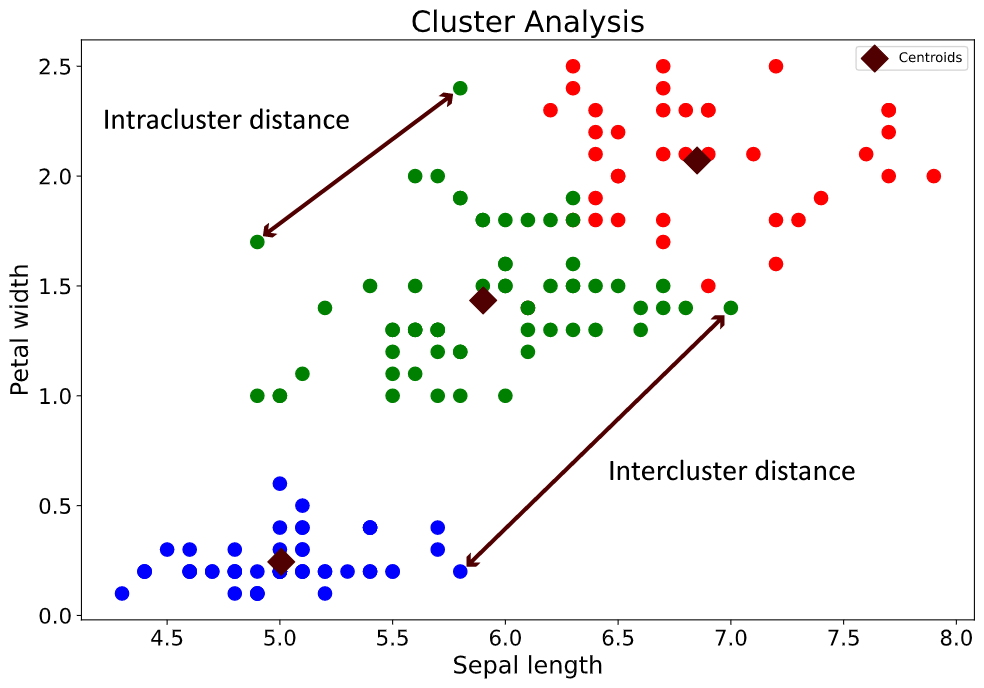
\includegraphics[width=\textwidth]{images/chapitre6/iris_inter_intra_clusters.png}
	\end{center}
\caption{Distances intracluster et intercluster.}
\label{inter_intra_clusters}
\end{figure}

\subsection{Distance inter-cluster}
La distance inter-cluster est la distance entre deux objets appartenant à deux clusters différents. Il y’a 5 types de distance inter-cluster :

\subsubsection{Distance de liaison unique}
La distance de liaison unique est la distance la plus proche entre deux objets appartenant à deux clusters différents. Le clustering de liaison unique est basé sur le critère de connectivité. La distances entre deux clusters \(\displaystyle S \) et \(\displaystyle T \) est : \cite{maulik2002performance}

% \begin{figure}[!h]
%     \centering
%     \subfloat[\centering les points de données en 2 dimensions]{{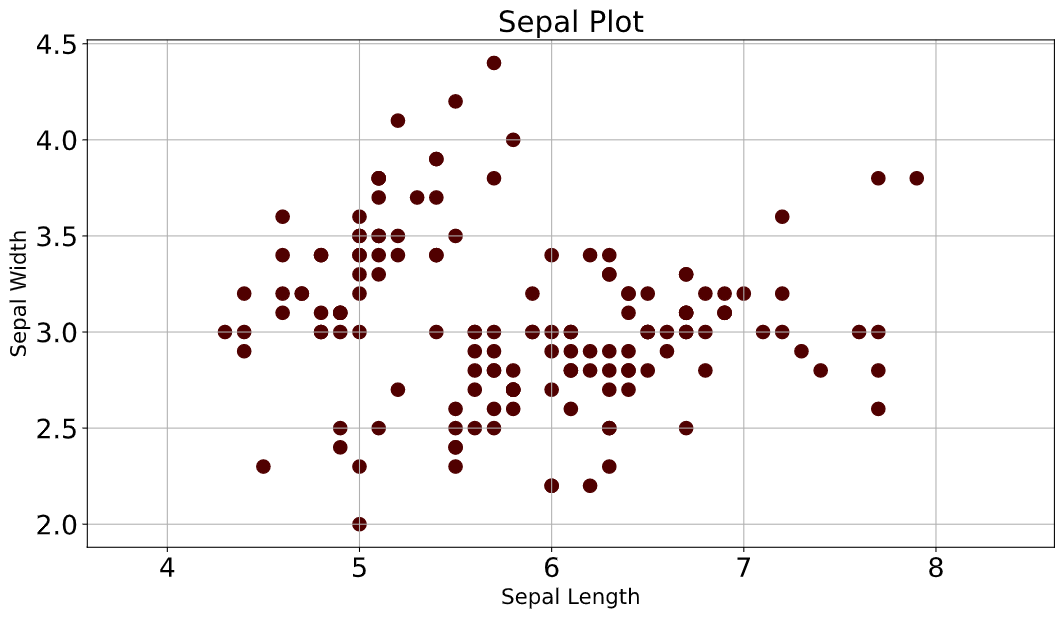
\includegraphics[width=7cm]{images/chapitre6/data_for_fuzzy.png} \label{data_for_fuzzy} }}%
%     \qquad
%     \subfloat[\centering Dendrogramme]{{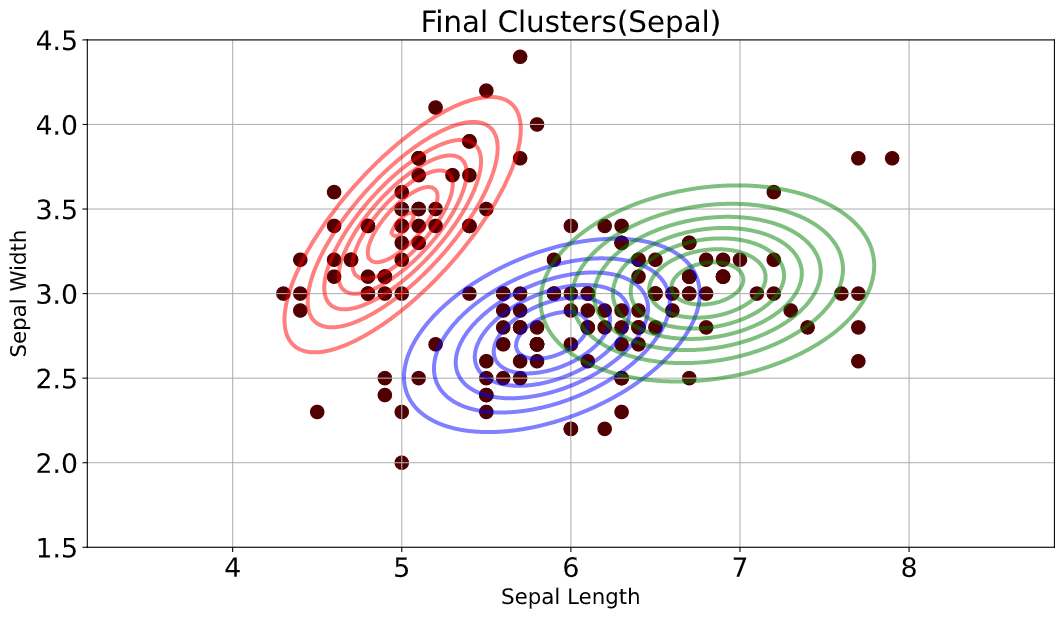
\includegraphics[width=7cm]{images/chapitre6/fuzzyExemple.png} } \label{fuzzy_example}}%
%     %\caption{Dendrogramme}%
% \end{figure}

\begin{equation}
	\vcenter{\hbox{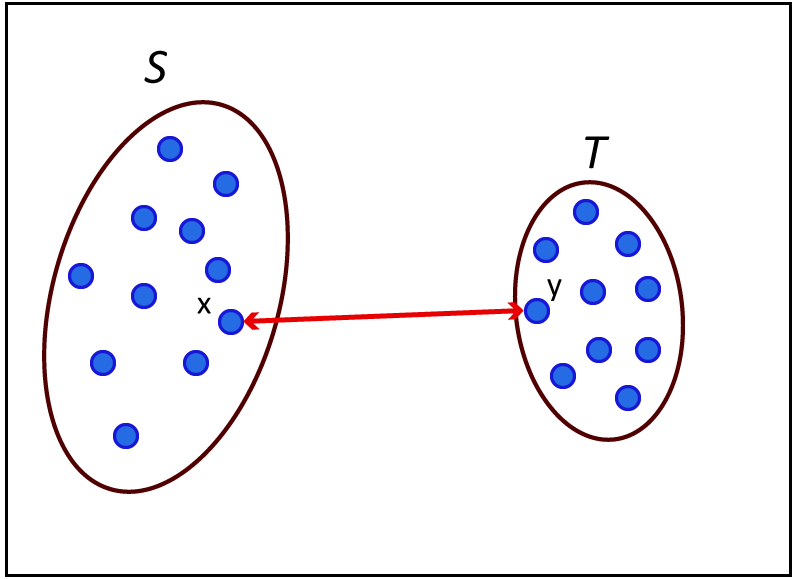
\includegraphics[scale=0.3]{images/chapitre6/single_linkage.png}}}
	\qquad
	\begin{aligned}
		 \delta (S,T) = \min  \Bigg\{
	\begin{tabular}{@{}l@{}}
		\(\displaystyle d(x,y) \)  \\
		\(\displaystyle x \in S,y \in T \) 
	\end{tabular} \Bigg\}
	\end{aligned}
	\label{signle_linkage_illust}
\end{equation}
% \begin{figure}[H]
% 	\begin{center}
% 		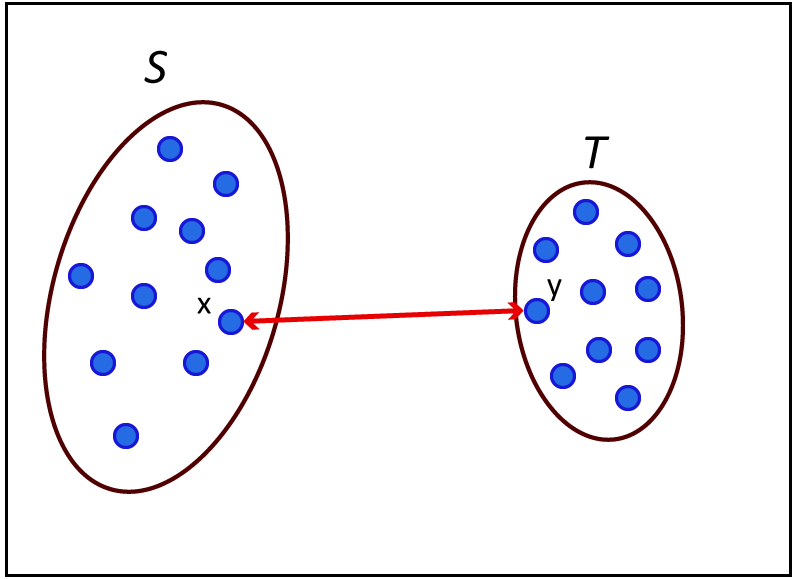
\includegraphics[width=\textwidth]{images/chapitre6/single_linkage.png}
% 	\end{center}
% \caption{Distances intracluster et intercluster.}
% \label{signle_linkage_illust}
% \end{figure}

% \begin{equation}
%      \delta (S,T) = \min  \Bigg\{
% \begin{tabular}{@{}l@{}}
%     \(\displaystyle d(x,y) \)  \\
%     \(\displaystyle x \in S,y \in T \) 
% \end{tabular} \Bigg\}
% \end{equation}

Le principal avantage de la liaison simple est qu'elle peut gérer des formes non elliptiques \cite{kumar2014performance}. Cependant, il est sensible au bruit et aux valeurs aberrantes \cite{jain1988algorithms} \cite{pang2005introduction}.

\subsubsection{Distance de liaison complète}
La distance de liaison complète est la distance entre deux objets les plus éloignés appartenant à deux clusters différents. La liaison complète est la plus grande distance entre les points de données dans deux clusters S et T définit par la formule suivante :

\begin{equation}
	\vcenter{\hbox{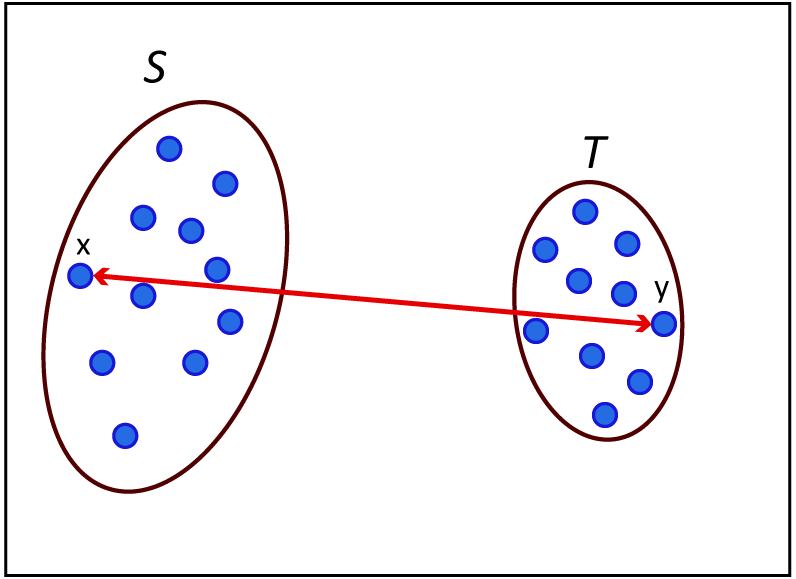
\includegraphics[scale=0.3]{images/chapitre6/complet_linkage.png}}}
	\qquad
	\begin{aligned}
		\delta (S,T) = \max  \Bigg\{
	\begin{tabular}{@{}l@{}}
	\(\displaystyle d(x,y) \)  \\
	\(\displaystyle x \in S,y \in T \) 
	\end{tabular} \Bigg\}
	\end{aligned}
	\label{complet_linkage_illust}
\end{equation}


% \begin{figure}[H]
% 	\begin{center}
% 		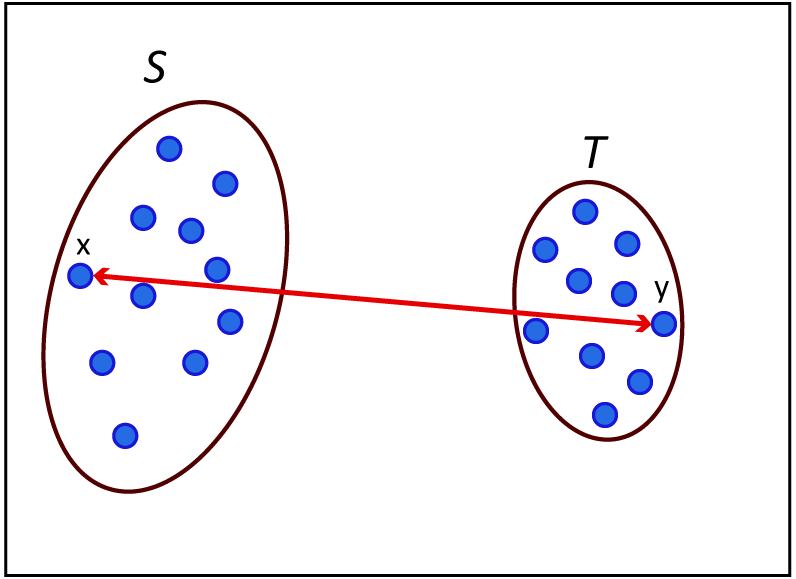
\includegraphics[width=\textwidth]{images/chapitre6/complet_linkage.png}
% 	\end{center}
% \caption{Distances intracluster et intercluster.}
% \label{complet_linkage_illust}
% \end{figure}

% \begin{equation}
% 	\delta (S,T) = \max  \Bigg\{
% \begin{tabular}{@{}l@{}}
%    \(\displaystyle d(x,y) \)  \\
%    \(\displaystyle x \in S,y \in T \) 
% \end{tabular} \Bigg\}
% \end{equation}

Cette distance ne tient pas compte de la structure du cluster et ne peut pas détecter les amas non sphériques \cite{kumar2014performance}.
\subsubsection{Distance de liaison moyenne}
La distance de liaison moyenne est la distance moyenne entre tous les objets appartenant à deux clusters différents. Le clustering de liaison moyenne a une procédure similaire que celle à liaison unique sauf le calcul de la distance entre deux clusters. Il utilise la moyenne entre les points de deux clusters S et T comme suit \cite{kumar2014performance} :

\begin{equation}
	\begin{split}
		\delta (S,T) = \frac{1}{\left\lvert S \right\rvert \left\lvert T \right\rvert  } \sum_{_{ x \in S},_{y \in T}} d(x,y)  \\
	\end{split}
\end{equation}
Le clustering utilisant la liaison moyenne est moins sensible au bruit et aux valeurs aberrantes. Le seul inconvénient est sa polarisation vers les amas globulaires \cite{pang2005introduction}.

\subsubsection{Centroïde Linkage Distance}
La distance de liaison centroïde est la distance entre les centres vs et vt de deux clusters S et T respectivement, définie comme :

\begin{equation}
	\begin{tabular}{@{}l@{}}
		\(\displaystyle \delta (S,T) = d(v_{s}, v_{t} ) \) où \\ \\
		\(\displaystyle v_{s} = \frac{1}{\left\lvert S \right\rvert}  \sum_{x \in S} x,v_{t} = \frac{1}{\left\lvert T \right\rvert} \sum_{y \in T}y  \) 
	\end{tabular} 
\end{equation}

\subsubsection{Distance de liaison moyenne du centre de gravité}
La distance de liaison moyenne du centre de gravité est la distance entre le centre d'un cluster et tous les objets appartenant à un autre cluster, définie comme :

\begin{equation}
	\delta (S,T) = \frac{1}{\left\lvert S \right\rvert  + \left\lvert T \right\rvert  }  \Bigg\{
\begin{tabular}{@{}l@{}}
   \(\displaystyle \sum_{x \in S} d(x,vt) + \sum_{y \in T}d(y,vs) \)
\end{tabular} \Bigg\}
\end{equation}

\subsection{Distance intra-cluster}
La distance intra-cluster est la distance entre deux objets appartenant au même cluster. Il y’en a trois types :

\subsubsection{Distance de diamètre complet}
La distance de diamètre complet est la distance entre deux objets les plus éloignés appartenant au même cluster défini comme :

\begin{equation}
	\begin{split}
		\Delta (S) = \max_{x,y \in S} \{ d(x,y) \}  \\
	\end{split}
\end{equation}

\subsubsection{Distance de diamètre moyen}
La distance de diamètre moyen est la distance moyenne entre tous les objets appartenant au même cluster défini comme :

\begin{equation}
	\begin{split}
		\Delta (S) = \frac{1}{\left\lvert S \right\rvert \cdot  (\left\lvert S \right\rvert - 1)} \sum_{x,y \in S ; x \neq y} \{ d(x,y) \} \\
	\end{split}
\end{equation}

\subsubsection{Diamètre barycentre Distance}
La distance de diamètre barycentre est à double distance moyenne entre tous les objets et le centre de groupe de s défini comme :

\begin{equation}
	\Delta (S) = 2  \Bigg \{
	\frac{\sum_{x \in S}d(x,\overline{v})}{\left\lvert S \right\rvert } \Bigg\} 
	\hspace{20pt} où \hspace{10pt} \overline{v} = \frac{1}{\left\lvert S \right\rvert} \sum_{x \in S}x
\end{equation}

\section{Le clustering hiérarchique}
\subsection{Introduction}
Dès les années 1970, on a estimé qu'environ 75\% de tous les travaux publiés sur le clustering utilisaient des algorithmes hiérarchiques \cite{murtagh2012algorithms}. Le clustering hiérarchique est une méthode de clustering qui permet d’identifier des clusters dans un ensemble de données. Contrairement aux autres méthodes de clustering comme le k-means, le clustering hiérarchique n’oblige pas à spécifier à l’avance le nombre de clusters à générer. Et le résultat est une représentation arborescente des observations, appelée dendrogramme. L'interprétation des informations contenues dans un dendrogramme est souvent d'un ou plusieurs types : relations d'inclusion d'ensemble, partition des ensembles d'objets et clusters significatifs \cite{murtagh2012algorithms}. C’est une méthode de clustering d’apprentissage automatique non supervisé qui procède à une décomposition de données en cherchant à construire une hiérarchie de clusters. Cette méthode suit deux approches basées sur la direction du progrès, c'est-à-dire s'il s'agit du flux descendant ou ascendant de création de clusters. Il s'agit respectivement de l'Approche Divisive et de l'Approche Agglomérative. \\
Le clustering agglomératif commence à partir des clusters singleton et obtient une hiérarchie en fusionnant successivement les clusters, tandis que le clustering divisif commence par un cluster unique contenant tous les points et se poursuit en fractionnant les clusters de manière itérative \cite{gurrutxaga2010sep}. le clustering hiérarchique crée donc une décomposition hiérarchique de l'ensemble de données.

\subsection{Clustering hiérarchique agglomératif}
En clustering, l'un des algorithmes les plus largement utilisés est les algorithmes agglomératifs. Il s'agit d'une approche « ascendante » : chaque observation commence dans son propre cluster, et les paires de clusters sont fusionnées au fur et à mesure que l'on monte dans la hiérarchie. Les résultats de la classification hiérarchique sont généralement présentés dans un dendrogramme. Cependant, pour certains cas particuliers, des méthodes agglomératives efficaces optimales (de complexité) sont connues : SLINK pour une liaison simple et CLINK pour un clustering à liaison complète \cite{sasirekha2013agglomerative}.
L’algorithme de clustering AHC a trois mesures de distance principales : liaison unique, liaison complète et liaison moyenne. Il est également appelé l’algorithme de clustering du plus proche voisin lorsque le critère single-linkage (liaison unique) est utilisée pour mesurer la distance distance entre les clusters \cite{zhou2016method}.
Dans le clustering hiérarchique agglomératif classique, une paire de clusters à fusionner à la distance minimale inter-cluster \cite{wu2004clustering}.

\subsubsection{Exemple de clustering agglomératif}

Par exemple, supposons que les données de la figure \ref{agglo_clustering} doivent être regroupées et que la métrique de distance est la distance euclidienne.
Le dendrogramme obtenu après le clustering serait comme tel : \ref{dendrogramme} \\
Et pour obtenir le nombre de clusters optimal avec le dendrogramme, la méthode la plus connue est celle qui cherche la distance verticale la plus élevée qui ne croise aucun cluster et les lignes verticales franchissent le seuil représente le nombre optimal de clusters. En utilisant le dendrogramme précédant on obtient 2 clusters comme le montre la figure \ref{dendrogramme}.

\begin{figure}[H]
	\centering
    \subfloat[\centering Les éléments du dataset.]{{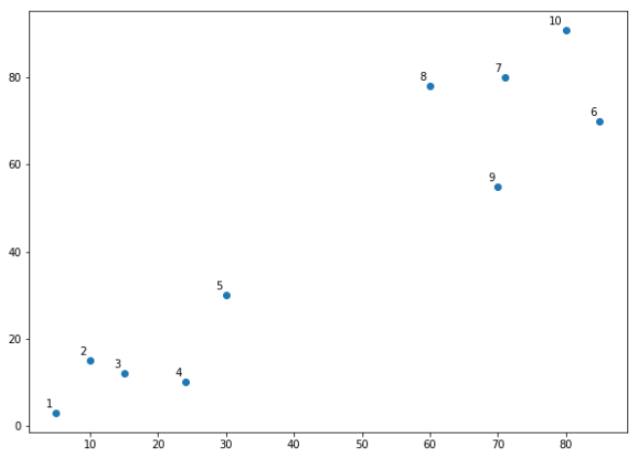
\includegraphics[width=7cm]{images/chapitre6/agglo_clustering.png} \label{agglo_clustering} }}%
    \qquad
    \subfloat[\centering Le dendrogramme.]{{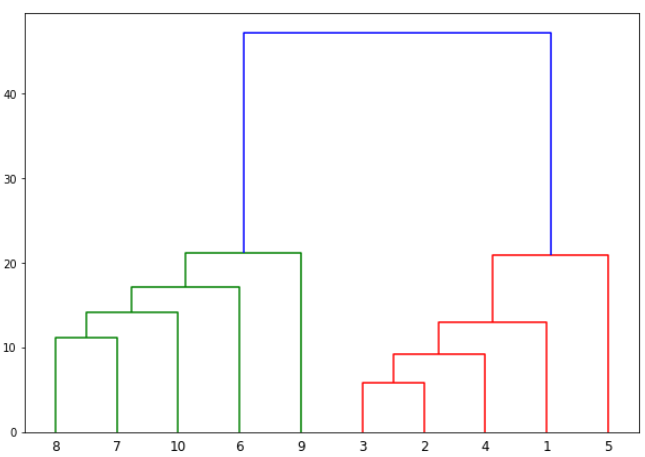
\includegraphics[width=7cm]{images/chapitre6/dendrogram.png} } \label{dendrogramme}}%
    %\caption{Dendrogramme}%
\end{figure}


\subsection{Clustering hiérarchique divisive}
Le principe de base du clustering divisif a été publié sous le nom d'algorithme DIANA (Divisive Analysis Clustering) \cite{Finding_Groups_in_Data_An_Introduction_To_Cluster_Analysis}. Contrairement au clustering hiérarchique agglomératif, le clustering hiérarchique divisif suit une approche descendante dans laquelle tous les points de données appartiennent à un seul grand cluster et celui-ci est divisé en groupes plus petits en fonction d'une logique de terminaison ou d'un point au-delà duquel il n'y aura plus de division de points de données. Le principe du clustering divisif est illustrer par la figure ci-dessous. \\
Le fractionnement est effectué de manière récursive au fur et à mesure que l'on descend dans la hiérarchie et il existe \(\displaystyle 2^{n-1}-1 \) \cite{edwards1965method}  façons de diviser un ensemble de n objets en deux sous-ensembles \cite{roux2018comparative}. Par conséquent le fractionnement prend top du temps sur la recherche de toutes les bipartitions possibles. Le clustering hiérarchique divisif procède par le fractionnement des clusters en deux clusters les moins similaires en utilisant des critères de type distance ou rapport et ensuite détermine les niveaux des nœuds (qui représente les groupes obtenus dans le dendrogramme).

\begin{figure}[H]
	\begin{center}
		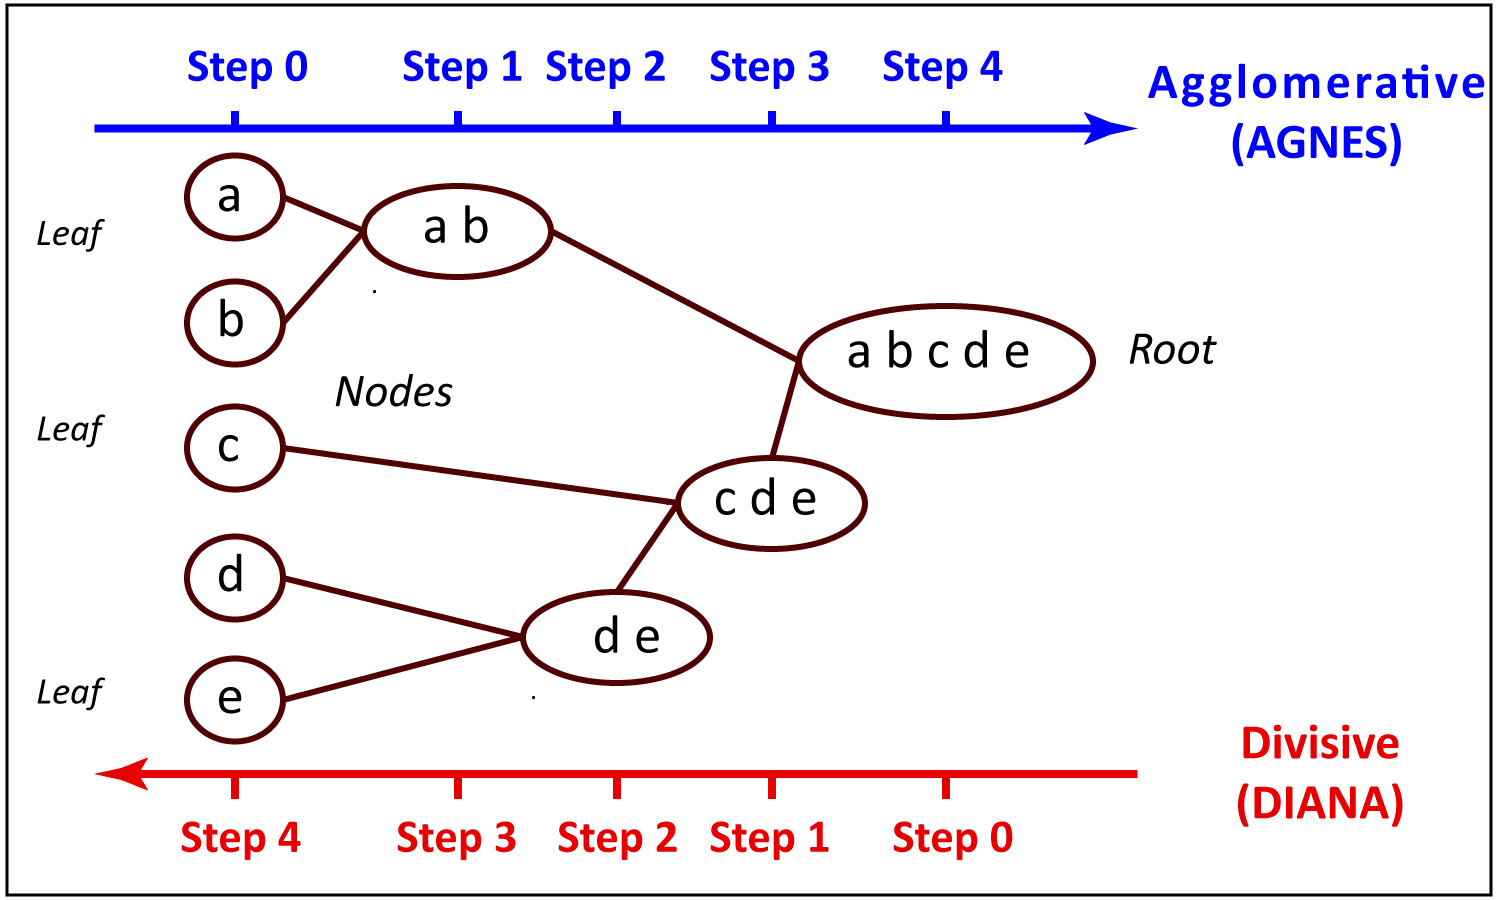
\includegraphics[scale=0.15]{images/chapitre6/hierarchical_agglo_divisive.png}
	\end{center}
\caption{La direction du clustering hiérarchique agglomérative et divisive.}
\label{hierarchical_agglo_divisive_illust}
\end{figure}

\subsection{Procédures de fractionnement des clusters}
Un certain nombre de procédures de fractionnement ont été conçus dans le passé. La procédure de Williams Et Lambert (1959) \cite{williams1959multivariate} est dite monothéique dans le sens où les ensembles d’objets sont divisé en fonction des valeurs d’une seule variable. Cette idée a été mise à jour en utilisant une composante principale au lieu d’une seule variable (algorithme Principal Directions Divisive Partitioning ou PDDP par Boley 1997) \cite{roux2018comparative}. \\
Une autre approche pour contourner la complexité du fractionnement consiste à extraire un ou plusieurs objets, de l’ensemble à fractionner. Macnaughton-Smith et al. (1964) \cite{macnaughton1964dissimilarity} ont proposé de sélectionner l’objet le plus distant comme center d’un nouveau cluster éloigné, puis les objets (les éléments du data set) les plus proche s’agrègent vers ce nouveau cluster \cite{roux2018comparative}. \\
Une idée similaire a été développée par Hubert (1973) \cite{hubert1973monotone}, qui suggéré d’utiliser une paire d’objets comme point d’origine de la nouvelle bipartition. Son choix a été de sélectionner les deux objets qui sont les plus dissemblables, puis de construire les deux sous-clusters en fonction des distances à ces points d’origines \cite{roux2018comparative}. \\
Exploitant cette idée, Roux \cite{roux1991basic} \cite{roux1995divisive} considérait les bipartitions générées par toutes les paires d'objets, en conservant la bipartition avec la meilleure évaluation de certains critères a priori \cite{roux2018comparative}. \\

\subsection{Evaluations des bipartitions}
Quel que soit le critère retenu, une série de très bonnes bipartitions ne se traduit pas automatiquement par une bonne hiérarchie. Les critères qui permettent d’évaluer les bipartitions sont de deux types : critère de type distance et les critères de type rapport. L’idée est donc de prendre en compte non seulement les dissemblances entre les clusters, mais aussi les dissemblances avec les éléments de deux clusters. Ces critères qui sont appelé aussi indice de validité sont énoncé dans le tableau \ref{validity_index_hard}.

\subsection{Déterminations de niveaux de nœuds }
Pour l’algorithme agglomératif, la valeur de l’indice de validité obtenu pour l’estimation du nombre optimale de clusters devient le niveau du nœud correspondant, et le dendrogramme ne montre aucun croisement (ou inversion) des branches. Malheureusement, les procédures qui divisent, en général, ne bénéficient pas de cette propriété, en raison du non-optimalité des fractionnements successifs. Une règle est alors nécessaire pour obtenir des niveaux cohérents et une véritable représentation arborescente \cite{roux2018comparative}.
\subsection{Conclusion}
Le clustering hiérarchique dans la recherche d'informations identifie donc des groupements ou regroupements des « objets » étudiés qui représentent le mieux certaines relations de similitude. Il permet ainsi d’obtenir des résultats dans une hiérarchie de cluster appelé dendrogramme. Et si le dendrogramme ne présente aucun croisement des branches, la visualisation de ce dernier permet de voir comment les différents sous-clusters sont liés les uns aux autres et à quelle distance sont les points de données.
\section{Le clustering partitionnel}

\subsection{K-means clustering}
K-means est un algorithme de clustering qui est largement utiliser pour analyser les clusters des grands ensembles de données. Il a été proposé par MacQueen en 1967 et c’était l’un des algorithmes d’apprentissage non supervisé le plus simple, qui a été appliqué pour résoudre les problèmes du clustering \cite{sun2008clustering}. Il s'agit d'un algorithme de partitionnement des clusters, cette méthode consiste à classer les objets d’un jeu de donnés en k clusters différents, de telle sorte que les clusters générés sont compacts et indépendants \cite{na2010research}.

\subsubsection{Le fonctionnement de l’algorithme k-means}
K-Means clustering fonctionne de cette façon : par exemple pour regrouper les données en trois clusters on commence par placer trois point appelé centroïde au hasard dans le jeu de données ensuite on affecte chaque point de data set au centroïde le plus proche ce qui nous donne trois clusters puis on déplace chaque centroïde au milieu de son cluster, on recommence jusqu’à ce que les centroïdes converge vers une position d’équilibre. L’algorithme requière donc à l’initialisation le nombre k de cluster à générer et k centroïdes (les centre des clusters) sont initialise avec des coordonnées aléatoires.

\subsubsection{Les étapes de l’algorithme}
L’algorithme de K-means clustering est un algorithme itératif qui procède comme suit :

\begin{itemize}
	\item	Sélection de k clusters a génère, où la valeur k est fixée à l'avance.
	\item	Initialisation des centroïdes avec de coordonnées aléatoires.
	\item	Calcul de la distance entre les objets et le centre de gravité du cluster.
	\item	Affectation des points au centroïde le plus proche.
	\item	Déplacement du centroïde à la moyenne du cluster.
	\item	Répétition des étapes précédente jusqu'à ce qu'il n'y ait pas de changement au centre des clusters.
\end{itemize}

Les étapes sont illustrées par la figure ci-dessous.

\begin{figure}[H]
	\begin{center}
		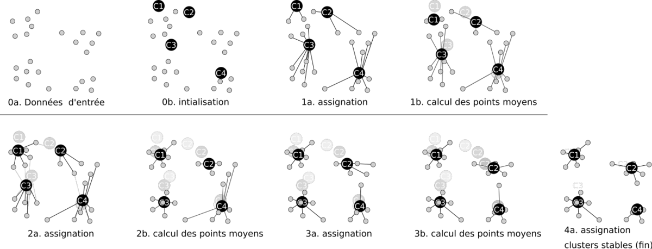
\includegraphics[width=\textwidth]{images/chapitre6/kmeans_steps.png}
	\end{center}
	\caption{Les étapes de l'algorithme k-means.}
	\label{kmeans_steps}
\end{figure}

Apres l’initialisation du nombre k des clusters a trouvées dans le jeu de données et k centroïdes, la distance euclidienne est généralement considérée pour déterminer la distance entre chaque objet de données et les centres du cluster. Cette distance est utilisée pour regrouper chaque objet de données au centre le plus proche \cite{fahim2006efficient}. La distance euclidienne entre un vecteur \(\displaystyle X = (x_{1},x_{2},x_{3},.....,x_{n}) \)  et un autre vecteur \(\displaystyle Y = (y_{1},y_{2},y_{3},.....,y_{n}) \), La distance euclidienne \(\displaystyle d(x_{i},y_{i})\) peut être obtenue comme suit:
\begin{equation}
    d(x_{i}, y_{i}) = \left[\sum_{i=1}^{n}(x_{i} - y_{i})^{2} \right]^{\frac{1}{2}}
\end{equation}

Lorsque tous les objets de données sont inclus dans certains clusters, la première étape est terminée et un regroupement précoce est effectué. Ce processus itératif continue jusqu'à ce que la fonction de critère est minimisé. \cite{na2010research}. \\
En supposant que l'objet cible est \(\displaystyle x \),\(\displaystyle x_{i} \) indique la moyenne du cluster \(\displaystyle C_{i} \), la fonction critère est définie comme suit :

\begin{equation}
    E = \sum_{i=1}^{k} \sum_{x \in C_{i}} \left\lvert x - x_{i} \right\rvert^{2}
\end{equation}

\subsubsection{Les lacunes de l’algorithme k-means}
L'algorithme de clustering k-means converge toujours vers le minimum local. Avant qu’il ne converge, l'algorithme doit calculer la distance entre chaque objet de données et chaque centre de cluster dans chaque itération. Du au choit aléatoire des centres de cluster initiaux, la valeur precise \(\displaystyle t \) connu sous le nom de nombre d'itérations k-means varie en fonction des centres de cluster de départ \cite{nazeer2009improving}. Aussi le fait de devoir choisir a priori le paramètre \(\displaystyle K \) est un inconvénient, car l’algorithme peut données des fausses informations sur les clusters générés et il est influencé par des valeurs aberrantes appelé aussi en anglais outliers.

\subsubsection{Les solutions aux lacunes de l’algorithme k-means}

Il n’est pas nécessaire de calculer la distance entre chaque objet de données et chaque centre de cluster dans chaque itération. En supposant que le cluster \(\displaystyle C \) s'est formé après le premier l' itération \(\displaystyle j \), l'objet de données \(\displaystyle x \) est affecté au cluster \(\displaystyle C \), mais dans quelques itérations, l'objet de données \(\displaystyle x \) est toujours affecté au cluster C. Donc si on constate que la distance de l'objet de données \(\displaystyle x \) aux autre cluster est petite que au cluster \(\displaystyle C \), il est possible d’arrêter le calcul de la distance lié l’objet x, car ceci provoque un long temps d'exécution affectant ainsi l'efficacité du clustering \cite{na2010research}. \\

Selon la position initiale des centroïdes, K-means peut donner de mauvais clusters. La configuration des clusters trouver par K-means peut ne pas être la plus optimale. On parle d’optimum local. La solution est d’exécuter K-means avec différentes positions de d´épart des centroïdes. La solution retenue est celle qui minimise la somme des distances entre les points \(\displaystyle (x) \) d’un cluster et son centre \(\displaystyle (u) \). Cela équivaut à minimiser la variance des clusters. K-means cherche la position des centroïdes qui minimise la distance entre les points
d’un cluster \(\displaystyle (X_{i}) \) et le centre \(\displaystyle (U_{i}) \) de ce dernier. L'algorithme de K-means cherche donc à minimise une fonction cout appeler Inertie et qui représente la distance entre le point d’un cluster et le centre de ce dernier. Les paramètres de la méthode kmeans() à optimiser pour le langage R :

\begin{itemize}
	\item  \textbf{Centers :} les clusters obtenus par l’algorithme son plus cohérant lorsque le nombre de centers demander par l’algorithme est le même que celui des clusters naturels du data set. Dans un data set avec de nombreuses dimensions il est difficile de voir un nombre de clusters à l’œil nu. Pour choisir le bon nombre de cluster il faut utiliser la méthode Elbow qui consiste à tracer l’évolution du cout du model en fonction du nombre de cluster et de détecter une zone de coude, cette zone nous indique le nombre de cluster optimale. C’est-`a-dire celui qui nous permet de réduire au maximum le cout du model tout en conservant un nombre raisonnable de cluster.
\end{itemize}

\begin{figure}[H]
	\begin{center}
		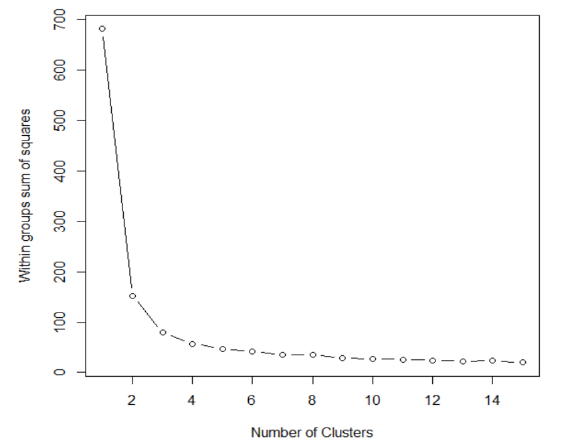
\includegraphics[scale=0.5]{images/chapitre6/elbow_methods.png}
	\end{center}
	\caption{La méthode Elbow.}
	\label{elbow_methods}
\end{figure}

\begin{itemize}
	\item	\textbf{nstart :} avec le nombre donner au paramètre nstart l’algorithme tente plusieurs configuration initial de la position des centroïdes et retient la meilleurs configuration qui minimise la variance des cluster. La valeur par défaut est 1 mais la valeur recommander est 25 par contre cette valeur conduit `a un gaspillage de ressource avec un grand data set.
	\item	\textbf{Iter.max :} le nombre de fois que l’algorithme doit s’exécuter. La valeur par défaut est 10 ce qui permet au centroïdes de converger ver position d’équilibre.
	\item	\textbf{algorithm :} l’algorithme choisit est celui qui donne une plus forte cohérence des clusters. Avec python l’algorithme kmeans++ donne des meilleurs résultats.

\end{itemize}

\section{Fuzzy clustering}
\subsection{Introduction}
Les méthodes de clustering traditionnelles (Hard) se limitent du fait que chaque point de l'ensemble de données appartient à un seul cluster. La théorie des ensembles flous proposée par Zadeh \cite{zadeh1965information} en 1965 a fait jaillir le concept d'incertitude d'appartenance, qui est décrit par la fonction d'appartenance \cite{yang1993survey}. L'utilisation d'ensembles flous fournit des informations d'appartenance de classe imprécises. L'application de la théorie des ensembles flous dans l'analyse de cluster a été proposée pour la première fois dans les travaux de Bellman, Kalaba et Zadeh \cite{zadeh1965information} et Ruspini \cite{ruspini1969new}. \\
Ruspini a proposé l'utilisation d'ensembles flous dans le clustering sous la forme d'une fonction objective qui obtient une meilleure partition floue des données en utilisant des méthodes Fuzzy (flou). Et cette méthode devient un problème d’optimisation de de fonction objective qui appartient à la catégorie du clustering flou basé sur les fonctions objectives. Il existe aussi le clustering flou basé sur une relation floue et le clustering « fuzzy generalized k-nearest neighbor rule ».\\
De nombreuses méthodes de regroupement flou ont été proposées en raison de modifications des fonctions objectives, qui visent à améliorer le résultat en ce qui concerne le bruit, les valeurs aberrantes, etc \cite{zhou2016method}. La methodes la plus est Fuzzy c-means (FCM) est une technique non supervisée qui classe les points de données similaires en clusters \cite{gurrutxaga2010sep}.\\
Dans de nombreuses situations, le clustering Soft est plus naturel que le clustering Hard parce que les objets situés aux limites entre plusieurs classes ne sont pas forcés d'appartenir entièrement à l'un des clusters, mais se voient plutôt attribuer des degrés d'appartenance compris entre 0 et 1 indiquant leur appartenance partielle. Au contraire, dans les techniques de clustering dur, les données sont groupées de manière exclusive, de sorte que si une certaine donnée appartient à un cluster défini, elle ne peut pas être incluse dans un autre cluster \cite{bora2014comparative}. Nous verrons dans cette section le Fuzzy c-means qui est une technique de clustering flou très populaire.\\

\subsection{Fuzzy C-means clustering :}
Fuzzy C-means (FCM) est une technique de regroupement de données dans laquelle chaque point de données appartient à un cluster dans une certaine mesure spécifiée par un degré d'appartenance. Cette technique a été initialement développé par Dunn 1973 et améliorer par Jim Bezdek en 1981 par rapport aux méthodes de clustering antérieures \cite{taherpour2018application}. Il fournit une méthode de regroupement des points de données qui peuplent un espace multidime nsionnel dans un nombre spécifique de clusters différents. Le principal avantage de cette methodes est qu’elle fournit des appartenances graduelles de points de données à des clusters mesurés en degrés dans un intervalle [0,1]. Cela donne la flexibilité d'exprimer que les points de données peuvent appartenir à plus d'un cluster.
\subsubsection{Algorithme FCM :}
Le but est de minimiser la fonction objective définie comme suit :

\begin{equation}
    J_{m} = \sum_{i=1}^{N} \sum_{j=1}^{C} U_{ij}^{m} \left\lVert x_{i} - c_{j} \right\rVert^{2} \hspace{10pt} avec \hspace{10pt}  1 \leq m \textless \infty
\end{equation}
Où \(\displaystyle U_{ij} \) est le degré auquel une observation \(\displaystyle x_{i} \) appartient à un cluster \(\displaystyle j \), \(\displaystyle c_{j} \) est le centre du cluster \(\displaystyle j \) et \(\displaystyle m \) le fuzzifier.

On remarque que FCM differe de k-means  du fait que FCM utilise les valeurs d’appartance \(\displaystyle U_{ij} \) et le fuzzifier \(\displaystyle m \). La variable \(\displaystyle U_{ij}^{m} \) est inversement lié à la distance entre x et le centre de cluster et est défini par  :
\begin{equation}
    U_{ij}^{m} = \frac{1}{\sum_{k=1}^{C} \Bigg ( \frac{\left\lVert x_{i} - c_{j} \right\rVert }{\left\lVert x_{i} - c_{k} \right\rVert} \Bigg )^{\frac{2}{m-1}}}
\end{equation}
Le paramètre m est un nombre réel supérieur à 1 \(\displaystyle (1 \leq m \textless \infty) \) et il définit le niveau de flou du cluster. Une valeur de \(\displaystyle m \) proche de 1 donne une solution de cluster qui devient de plus en plus similaire à la solution de clustering \textbf{Hard} tel que k-means ; alors qu’une valeur de m proche de l’infini conduit à un flou complet. Le bon choix est d’utiliser \(\displaystyle m = 2.0 \)  (Hathaway et Bezdek 2001). \\
Enfin le centroïde d’un cluster est la moyenne de tous les points, pondérée par leur degré d’appartenance au cluster. 

\begin{equation}
    C_{j} = \frac{\sum_{i = 1}^{N} U_{ij}^{m} \cdot x_{i}}{ \sum_{i=1}^{N} U_{ij}^{m}}
\end{equation}

\begin{figure}[!h]
    \centering
    \subfloat[\centering Les éléments du dataset Iris \cite{iris_dataset}.]{{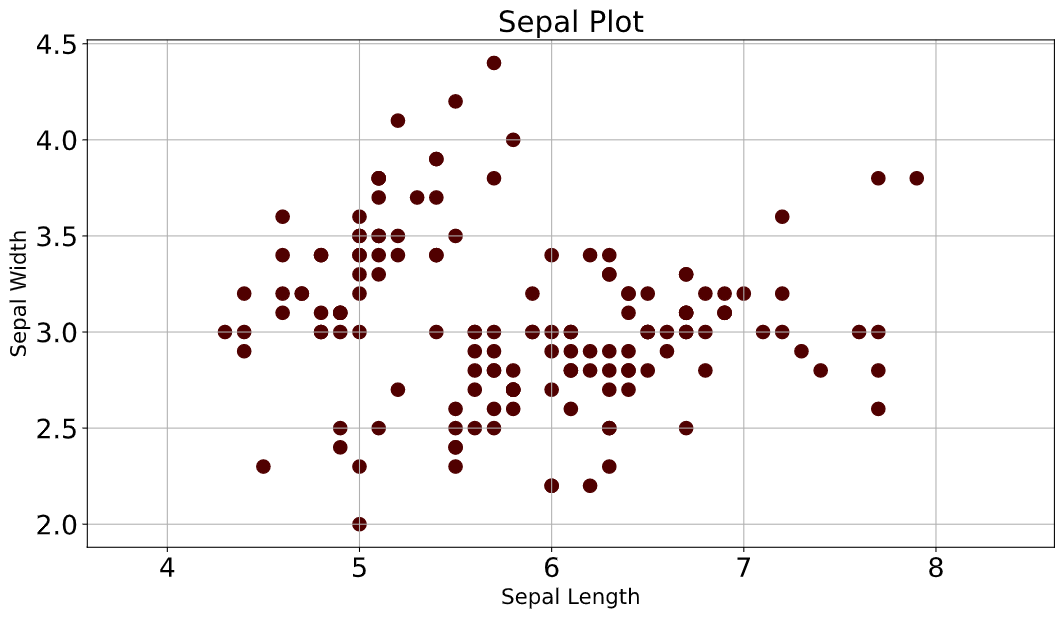
\includegraphics[width=7cm]{images/chapitre6/data_for_fuzzy.png} \label{data_for_fuzzy} }}%
    \qquad
    \subfloat[\centering Illustration du degré d’appartenance des éléments au cluster.]{{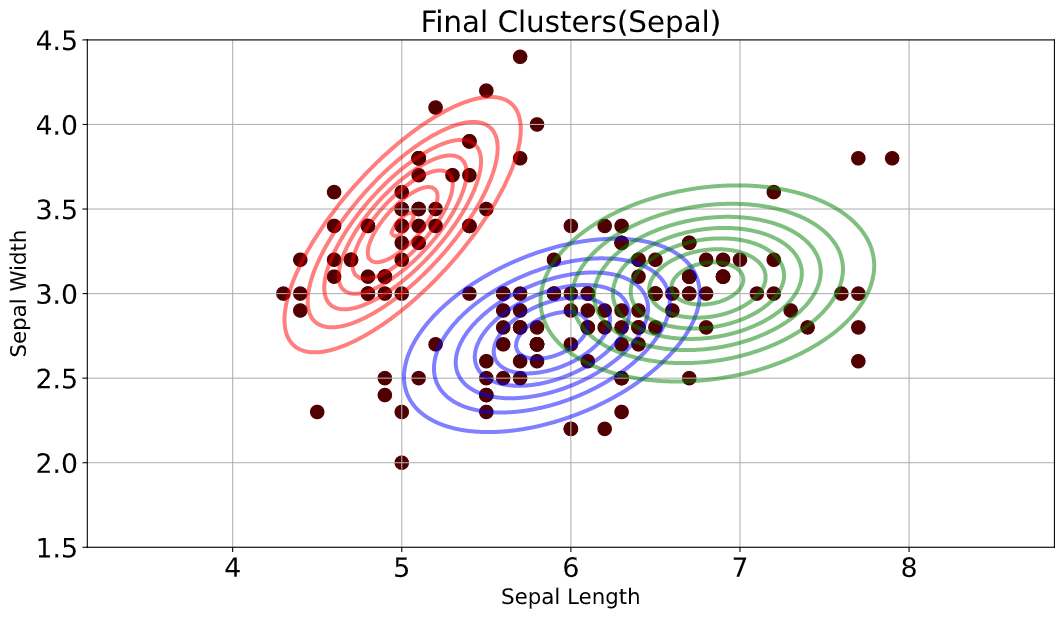
\includegraphics[width=7cm]{images/chapitre6/fuzzyExemple.png} } \label{fuzzy_example}}%
    %\caption{Dendrogramme}%
\end{figure}

\subsection{Conclusion}
Le clustering flou c-means peut être considéré comme un meilleur algorithme par rapport à l'algorithme k-Means. Contrairement à l'algorithme k-Means où les points de données appartiennent exclusivement à un cluster, dans le cas de l'algorithme flou c-means, le point de données peut appartenir à plus d'un cluster avec une vraisemblance ou une probabilité. Le regroupement flou c-means donne des résultats comparativement meilleurs pour les ensembles de données qui se chevauchent.

\section{Les autres méthodes de clustering}
En dehors des méthodes de clustering hiérarchique, partitionnel et floue (fuzzy) vu précédemment, les autres méthodes de clustering sont énoncées de façon brève dans le tableau \ref{other_clustering_methods} . 
\begin{table}[H]
	\centering
	\addtolength{\leftskip} {-4cm}
	\addtolength{\rightskip}{-3cm}
	\begin{tabular}{|m{3cm}|m{4cm}|m{5cm}|m{3cm}|m{3cm}|} %\rule{0pt}{1.5\normalbaselineskip}
	\hline
	\rowcolor{blueforest}
	\color{white} \textbf{Clustering Method} & \color{white} \textbf{Description} & \color{white} \textbf{Advantages} & \color{white} \textbf{Disadvantages} & \color{white} \textbf{Algorithms}\\
	\hline\hline
	\textbf{Distribution based Clustering}  & Basé sur la distribution de probabilité des données, les clusters sont dérivés de diverses métriques telles que la moyenne, la variance, etc. & Le nombre de clusters n'a pas besoin d'être spécifié a priori, fonctionne sur des données en temps réel, les métriques sont faciles à comprendre et à régler. & Algorithme complexe et lent, ne peut pas être adapté à des données plus volumineuses & Gaussian Mixed Models, DBCLASD\\ \hline
	\textbf{Density based Clustering (Model-based methods)} & Basé sur la densité des points de données, également connu sous le nom de clustering basé sur un modèle. & Peut gérer le bruit et les valeurs aberrantes, n'a pas besoin de spécifier le nombre de clusters au début, les clusters créés sont très homogènes, aucune restriction sur les formes de cluster.  & Algorithme complexe et lent, ne peut pas être adapté à des données plus volumineuses & DENCAST, DBSCAN \\ \hline
	\textbf{Constraint based (Supervised Clustering)} & Le clustering est dirigé et contrôlé par les contraintes & Crée une limite de décision parfaite, peut déterminer automatiquement les classes de résultats en fonction des contraintes, les données futures peuvent être classées en fonction des limites de formation. & Surapprentissage, niveau élevé d'erreurs de classification erronée, ne peut pas être entraîné sur des ensembles de données plus volumineux & Decision Trees, Random Forest, Gradient Boosting. \\ \hline
	\end{tabular}
	\caption{Les autres méthodes de clustering}
	\label{other_clustering_methods}
\end{table}

\section{La différence entre le clustering hiérarchique, partitionnel et Fuzzy clustering}
Le clustering hiérarchique et partitionnel présente des différences essentielles en termes de temps d’exécution, d’hypothèses, de paramètres d’entrée et de clusters résultants. En règle générale, le clustering partitionnel est plus rapide que le clustering hiérarchique. La classification hiérarchique nécessite uniquement une mesure de similarité, tandis que la classification partitionnelle requiert des hypothèses plus strictes telles que le nombre de classes et les centres initiaux. La mise en cluster hiérarchique ne nécessite aucun paramètre d’entrée, tandis que les algorithmes de mise en cluster partiels nécessitent le nombre de clusters à exécuter. La classification hiérarchique renvoie une division beaucoup plus significative et subjective des grappes, mais la classification partitionnelle produit exactement k clusters. Les algorithmes de classification hiérarchique conviennent mieux aux données catégoriques, à condition qu’une mesure de similarité puisse être définie en conséquence. En terme générale ils sont considérés comme des méthodes de clustering Hard, où chaque élément est affecté à un seul cluster. Par contre les méthodes de clustering Soft comme le Fuzzy clustering regroupent les éléments de données de telle sorte qu'un élément puisse exister dans plusieurs clusters.
\section{Indice de validité du clustering}
Les algorithmes supervisés ont beaucoup de métriques pour vérifier leur qualité d'ajustement comme la précision, la valeur r carré, la sensibilité, la spécificité, etc. Concernant les algorithmes non supervisés et plus précisément les algorithmes de clustering l’indice de validité de cluster est utilisé pour mesurer la qualité de la partition trouvée et aussi les partitions optimales. L’indice de validité de cluster est utilisé donc pour mesurer la qualité des clusters et pour rechercher le nombre optimal de clusters lorsque le nombre de clusters dans les données l'ensemble n'est pas connu à l'avance \cite{rezaee1998new}. Il utilise les propriétés des clusters telles que la compacité (ou la variation) et la séparation (ou l'isolement) qui sont souvent considérées comme des caractéristiques majeures permettant de valider les clusters. La compacité indique la variation ou la dispersion des données au sein d'un cluster, et la séparation indique l'isolement des clusters les uns des autres \cite{ZHANG20081205} . Plusieurs indices de validité courants sont énoncés dans le tableau suivant :
\begin{table}[H]
	\centering
	\addtolength{\leftskip} {-4cm}
	\addtolength{\rightskip}{-4.5cm}
	\begin{tabular}{|m{2cm}|m{5cm}|m{12cm}|}
	\hline
	\rowcolor{blueforest}
	\color{white} \textbf{Indice} & \color{white} \textbf{Description} & \color{white} \textbf{Formule}  \\
	\hline\hline
	\multicolumn{3}{|m{19cm}|}{\centering \textbf{Les indices de validité adaptés aux clustering partitionnelle} }\\ \hline
	\textbf{Indice de Dunn}  &
	Il est l'un des indices les plus anciens et les plus cités est proposé par \cite{dunn1974well}. L'index de Dunn (DU) identifie les clusters qui sont bien séparés et compacts. Le but est donc de maximiser la distance inter-clusters tout en minimisant la distance intra-cluster. &  \(\displaystyle DU_{k} = \min_{i=1,..,k} \Bigg \{ \min_{j=1+1,..,k} \Bigg ( \frac{diss(c_{i},c_{j})}{\max_{m=1,...,k}diam(c_{m})} \Bigg ) \Bigg \} \) \newline \newline où \(\displaystyle diss(c_{i},c_{j}) = \min_{x \in c_{i},y \in c_{j}}d(x,y) \) est la dissemblance entre les clusters \(\displaystyle c_{i} \) et \(\displaystyle c_{j}  \), et \(\displaystyle diam(C) = \max_{x,y \in C}d(x,y) \) est la fonction intra-cluster (ou diamètre) du cluster. Si l'index de Dunn est grand, cela signifie qu'il existe des clusters compacts et bien séparés \cite{Saitta2008}. \\ \hline
	\textbf{Indice Calinski-Harabasz}  &
	Cet indice \cite{calinski1974dendrite} est basé sur un rapport entre la matrice de dispersion des clusters (BCSM) et la matrice de dispersion des clusters (WCSM). &  \(\displaystyle CH_{k} = \frac{BCSM}{k-1} \cdot \frac{n-k}{WCSM} \) \newline où \(\displaystyle n  \) est le nombre total de points et \(\displaystyle k  \) le nombre de clusters. Le \(\displaystyle BCSM   \) est basé sur la distance entre les clusters et est défini par : \(\displaystyle BCSM = \sum_{i=1}^{k} n_{i} \cdot d(z_{i},z_{tot})^{2}  \), où \(\displaystyle z_{i}  \) est le centre du cluster \(\displaystyle c_{i}  \) et \(\displaystyle n_{i}  \) le nombre de points dans \(\displaystyle c_{i}  \). Le \(\displaystyle WCSM  \)  est : \(\displaystyle WCSM = \sum_{i=1}^{k} \sum_{x \in c_{i}} d(x,z_{i})^{2}  \) où \(\displaystyle x  \) x est un point de données appartenant au cluster \(\displaystyle c_{i}  \). Pour obtenir des clusters bien séparés et compacts, BCSM est maximisé et WCSM minimisé \cite{Saitta2008}. \\ \hline
	\textbf{Indice Davies-Bouldin} & Semblable à l'indice de Dunn, l'indice Davies-Bouldin \cite{davies1979cluster} identifie des clusters éloignés les uns des autres et compacte.  & \(\displaystyle DB_{k} = \frac{1}{k} \sum_{i=1}^{k} max_{j=1,...,k;i \neq j} \Bigg \{ \frac{diam(c_{i}) + diam(c_{j})}{d(z_{i},z_{j})} \Bigg \}  \) \newline où le diamètre d'un cluster est : \(\displaystyle diam(c_{i}) = \sqrt{\frac{1}{n_{i}} \sum_{x \in c_{i}} d(x,z_{i})^{2}}  \), avec \(\displaystyle n_{i}  \) le nombre de points et \(\displaystyle z_{i}  \) le centre de gravité du cluster \(\displaystyle c_{i}  \). Puisque l'objectif est d'obtenir des clusters avec des distances intra-clusters minimales, les petites valeurs de \(\displaystyle DB  \) sont intéressantes. Par conséquent, cet index est minimisé lors de la recherche du meilleur nombre de clusters \cite{Saitta2008}. \\ \hline
	\textbf{Indice de silhouette} & La statistique de silhouette \cite{kaufman2009finding} est une autre façon bien connue d'estimer le nombre de groupes dans une donnée ensemble. L'indice Silhouette (SI) calcule pour chaque point une largeur en fonction de son appartenance à groupe. Cette largeur de silhouette est alors une moyenne sur l'ensemble des observations.  & \(\displaystyle SI_{k} = \frac{1}{k} \sum_{i=1}^{n} \frac{(b_{i} - a_{i})}{\max (a_{i},b_{i})}  \), \newline où \(\displaystyle n  \) est le nombre total de points, \(\displaystyle a_{i}  \) est la distance moyenne entre le point \(\displaystyle i  \) et tous les autres points de son propre cluster et \(\displaystyle b_{i}  \) est le minimum des dissemblances moyennes entre \(\displaystyle i  \) et les points d'autres clusters. Enfin, la partition avec le \(\displaystyle SI  \) le plus élevé est considérée comme optimale \cite{Saitta2008}. \\ \hline
	\end{tabular}
	\caption{Indice de validité du clustering Hard}
	\label{validity_index_hard}
\end{table}

\begin{table}[H]
	\centering
	\addtolength{\leftskip} {-4cm}
	\addtolength{\rightskip}{-4.5cm}
	\begin{tabular}{|m{7cm}|m{12cm}|}
	\hline
	\rowcolor{blueforest}
	\color{white} \textbf{Indice} & \color{white} \textbf{Formule}  \\
	\hline\hline
	\multicolumn{2}{|m{19cm}|}{Il y’a aussi d’autre indice de validité de clustering partitionnel comme l’indice de Maulik-Bandyopadhyay et Geometric index. Les indices de validité utilisé pour le fuzzy clustering sont : }\\ \hline
	  \textbf{Le coefficient de partition \(\displaystyle PC \) \cite{bezdek1974numerical} }  & \(\displaystyle V_{PC} = \frac{1}{n} \sum_{i=1}^{c} \sum_{j=1}^{n} u_{ij}^{2} \) \\ \hline
	  \textbf{L'entropie de partition \(\displaystyle PE \) \cite{bezdek1973cluster} }  & \(\displaystyle V_{PE} = - \frac{1}{n} \sum_{i=1}^{c} \sum_{j=1}^{n} u_{ij} \log u_{ij} \) \\ \hline
	  \textbf{Fonction de validité proposée par Wu et Yang \cite{wu2005cluster} }  & \(\displaystyle V_{PCAES} = \sum_{i=1}^{c} PCAES_{i} = \sum_{i=1}^{c} \sum_{j=1}^{n}u_{ij}^{2}/u_{M} - \sum_{i=1}^{c} \exp (- \min_{k \neq i} \{ \left\lVert v_{i} - v_{k} \right\rVert^{2} / \beta_{T}   \} ) \) \newline où \(\displaystyle u_{M} = \min_{1 \leq i \leq  c} \Bigg \{ \sum_{j=1}^{n} u_{ij}^{2} \Bigg \}\), \(\displaystyle \beta_{T} = \frac{\sum_{l=1}^{c} \left\lVert v_{l} - \overline{v} \right\rVert^{2} }{c}   \) et \(\displaystyle \overline{v} = \sum_{j=1}^{n} x_{j}/n  \) \newline La grande valeur VPCAES signifie que les \(\displaystyle c  \) clusters sont compact et séparé les uns des autres, et la petite valeur VPCAES implique qu’ils ne sont pas compacts ou séparés.  \\ \hline
	  \textbf{Fonction de validité proposée par Fukuyama et Sugeno \cite{fukuyama1989new} }  & \(\displaystyle V_{FS} = J_{m}(U,V) - K_{m}(U,V) = \sum_{i=1}^{c}\sum_{j=1}^{n} u_{ij}^{m} \left\lVert x_{j} - v_{i} \right\rVert^{2} - \sum_{i=1}^{c}\sum_{j=1}^{n} u_{ij}^{m} \left\lVert v_{i} - \overline{v} \right\rVert^{2} \) , \newline où \(\displaystyle \overline{v} = \sum_{j=1}^{n} x_{j}/n \) . \\ \hline
	  \textbf{Fonction de validité proposée par Xie et Beni \cite{xie1991validity}  }  & \(\displaystyle V_{XB} = \frac{J_{m}(U,V)/n}{Sep(V)} = \frac{\sum_{i=1}^{c}\sum_{j=1}^{n} u_{ij}^{m} \left\lVert x_{j} - v_{i} \right\rVert^{2} }{n\min_{i \neq j} \left\lVert v_{i} - v_{j} \right\rVert^{2} } \) \\ \hline
	\end{tabular}
	\caption{Indice de validité du clustering Soft}
	\label{validity_index_soft}
\end{table}


\section{Conclusion}
Nous avons passé en revue dans cette partie le clustering qui est une méthode de l’apprentissage automatique non-supervisé et les techniques qu’il utilise pour l’extraction des clusters. Plusieurs objectif pousse à utiliser certaines techniques de clustering comme le clustering partitionnel et hiérarchique qui forme des clusters où chaque élément appartient à un seul cluster et le clustering flou (fuzzy) où chaque élément peut appartenir à plusieurs clusters avec un degré d’appartenance. Ensuite après l’extraction des clusters, les indices de validité de clusters peuvent être utilisé pour évaluer la qualité des clusters obtenue où détecter à l’avance le nombre de clusters optimale avant d’utiliser les algorithmes.
%%%%%%%%CONTRIBUTIONS%%%%%%%%%%
\secondpart

\chapter{Contribution and Results}
\minitoc
\thispagestyle{empty}
\newpage

\section{Introduction}
Nous présentons dans ce chapitre les notions vues dans les chapitres précédents appliquer à un dataset. Partant de la collecte et la préparation du dataset, de l’application de la théorie des réponses aux items pour un ajustement bayésiens des réponses obtenues par les apprenants, jusqu’aux clustering hard et soft des items basés sur la similarité.

\section{Approche proposée}


\section{Implémentations et résultats expérimentaux}

\subsection{Outils de développement}
les outils matériels et logiciels utilisés pour le développement sont :

\subsubsection{Materiels}

\begin{table}[H]
  \centering
  \begin{tabular}{cccc}
    \toprule
     \textbf{Marque} & \textbf{CPU} & \textbf{RAM} & \textbf{OS} \\
     \midrule
       \textbf{Lenovo Y40-80} & AMD Intel Core i5 2.20 GHz & 16Go & Windows10 64bits \\ \hline
       \multicolumn{4}{m{14cm}}{\centering Et Linux Ubuntu 20.04 LTS installé sur WSL2 }\\
    \bottomrule
  \end{tabular}
  \caption{Caractéristiques du matériels utilisés}
  \label{tabmat}
\end{table}

\textbf{WSL2 :} Windows Subsystem for Linux (WSL) est une couche de compatibilité permettant d'exécuter des exécutables binaires Linux de manière native sur Windows 10 et Windows Server 2019. WSL2 est une version améliorer de WSL1 qui introduit d'importants changements, notamment la présence d'un véritable noyau Linux \cite{craigloewen_msft} via un sous-ensemble de fonctionnalités Hyper-V. 

\subsubsection{Outils et packages}

\begin{table}[H]
	\centering
	\addtolength{\leftskip} {-4cm}
	\addtolength{\rightskip}{-4.5cm}
	\begin{tabular}{|m{5cm}|m{14cm}|}
	\hline
	\rowcolor{blueforest}
	\color{white} \textbf{Outils | Packages} & \color{white} \textbf{Description}  \\
	\hline\hline
	\multicolumn{2}{|m{19cm}|}{\centering Les outils et packages utilisés sur windows 10 : }\\ \hline
	\begin{center}
	    \begin{minipage}{.3\textwidth}
      
\includegraphics[width=\textwidth]{images/chapitre7/python.png}
    \end{minipage}
	\end{center}
	\centering \textbf{Python} \cite{10.5555/1593511} & Créé par le développeur Guido Van Rossum et publié pour la première fois en 1991. Il permet aux programmeurs d'utiliser différents styles de programmation pour créer des programmes simples ou complexes. Python est l'un des langages de programmation les plus populaires pour la science des données. C'est un langage de programmation de haut niveau, structuré, open source, interprété et dynamique. Il est multiparadigme, multi-plateforme et multi-usages. La syntaxe de Python aide les programmeurs à coder en moins d'étapes par rapport à d'autres langages comme JAVA ou C++, ce qui facilite le travail et le rend plus rapide, facile et amusant à faire. Il possède une bibliothèque standard complète et volumineuse dotée d'une gestion automatique de la mémoire et de fonctionnalités dynamiques \cite{python_cours}. Dans notre travail, nous avons utilisé Python 3.5 intégré à Anaconda. \\ \hline
  \begin{center}
	    \begin{minipage}{.3\textwidth}
      
\includegraphics[width=\textwidth]{images/chapitre7/anaconda.png}
    \end{minipage}
	\end{center}
	\centering \textbf{Anaconda} & Anaconda \cite{anaconda_citation} est une distribution libre et open source \cite{anaconda_website} des langages de programmation Python et R appliqué au développement d'applications dédiées à la science des données et à l'apprentissage automatique (traitement de données à grande échelle, analyse prédictive, calcul scientifique), qui vise à simplifier la gestion des paquets et de déploiement. Les versions de paquetages sont gérées par le système de gestion de paquets conda \cite{conda_website} et est adapté pour Windows, Linux et MacOS. Anaconda fournit interface graphique qui permet de lancer des applications, de gérer les librairies avec gestionnaire de paquets conda, et les environnements de développement. Plusieurs applications sont disponibles par défaut comme JupyterLab, Jupyter Notebook, QtConsole5, Spyder, Glue, Orange, RStudio, Visual Studio Code.  \\ \hline
  
  \begin{center}
    \begin{minipage}{.3\textwidth}
    
\includegraphics[width=\textwidth]{images/chapitre7/jupyter.png}
  \end{minipage}
  \end{center}
  \centering \textbf{Jupyter Notebook} \cite{Kluyver2016jupyter} & Jupyter Notebook est un environnement de programmation interactif basé sur le web utilisé pour programmer en python, R, Ruby, Julia ou encore Scala qui permet de réalisé des notebooks contenant à la fois du texte en markdown et du code en Julia, Python, R etc.  \\ \hline

  \begin{center}
    \begin{minipage}{.3\textwidth}
    
\includegraphics[width=\textwidth]{images/chapitre7/scikit_learn.png}
  \end{minipage}
  \end{center}
  \centering \textbf{Scikit-learn} \cite{pedregosa2011scikit} & Scikit-learn est une bibliothèque libre Python destinée à l'apprentissage automatique. Elle propose un ensemble d'outils efficace clé en main pour l’analyse et l’exploration de données. Cette bibliothèque prend en charge les algorithmes de classifications, de régression, du clustering, la réduction de dimensionnalité et de prétraitement des données pour l'extraction et la normalisation des caractéristiques.  \\ \hline

  \end{tabular}
	\caption{Indice de validité du clustering Hard}
	\label{tools}
\end{table}

\newpage

\begin{table}[H]
	\centering
	\addtolength{\leftskip} {-4cm}
	\addtolength{\rightskip}{-4.5cm}
	\begin{tabular}{|m{5cm}|m{14cm}|}
	\hline
	\rowcolor{blueforest}
	\color{white} \textbf{Outils | Packages} & \color{white} \textbf{Description}  \\
	\hline\hline
  %  >>>>>>>>>>>>>>
	\begin{center}
	    \begin{minipage}{.3\textwidth}
      
\includegraphics[width=\textwidth]{images/chapitre7/pandas.png}
    \end{minipage}
	\end{center}
  \centering \textbf{Pandas} \cite{mckinney2010data} & Pandas est une bibliothèque écrite en Python qui permet la manipulation et l'analyse des données. Elle propose en particulier des structures de données et des opérations de manipulation de tableaux numériques et de séries temporelles. Elle propose principalement comme structures de données les Series, DataFrames, Panels, Panels4D. Et aussi des fonctionnalités comme la manipuler des données aisément et efficacement avec des index pouvant être des chaines de caractères, des outils pour lire et écrire des données structurées, gestion des données manquantes, le tri, le redimensionnement et , fusion et jointure de large volume de données et analyse de séries temporelles. \\ \hline
  % <<<<<<<<<<<<<<

  %  >>>>>>>>>>>>>>
  \begin{center}
	    \begin{minipage}{.3\textwidth}
      
\includegraphics[width=\textwidth]{images/chapitre7/numpy.png}
    \end{minipage}
	\end{center}
	\centering \textbf{Numpy} \cite{2020NumPy-Array} & est une bibliothèque python pour le calcul scientifique qui fournit un objet tableau multidimensionnel, divers objets dérivés (tels que des tableaux et des matrices masqués) et un assortiment de routines pour des opérations rapides sur des tableaux, notamment mathématiques, logiques, manipulation de forme, tri, sélection, transformées de Fourier discrètes, algèbre linéaire de base, opérations statistiques de base, simulation aléatoire etc.  \\ \hline
  % <<<<<<<<<<<<<<
  \begin{center}
    \begin{minipage}{.3\textwidth}
    
\includegraphics[width=\textwidth]{images/chapitre7/matplotlib.png}
  \end{minipage}
  \end{center}
  \centering \textbf{Matplotlib} \cite{hunter2007matplotlib} & Matplotlib est une bibliothèque du langage de programmation Python destinée à tracer et visualiser des données sous formes de graphiques en 2 ou 3 dimensions \cite{tosi2009matplotlib}. Cette bibliothèque permet de produire divers tracés par exemple des histogrammes, des fonctions de Rosenbrock, spirale logarithmique, graphiques d'erreurs, nuages de points etc.  \\ \hline

  \end{tabular}
	\caption{Indice de validité du clustering Hard}
	\label{tools}
\end{table}

\newpage

\begin{table}[H]
	\centering
	\addtolength{\leftskip} {-4cm}
	\addtolength{\rightskip}{-4.5cm}
	\begin{tabular}{|m{5cm}|m{14cm}|}
	\hline
	\rowcolor{blueforest}
	\color{white} \textbf{Outils | Packages} & \color{white} \textbf{Description}  \\
	\hline\hline
	\multicolumn{2}{|m{19cm}|}{\centering Les outils et packages supplémentaires utilisés sur Linux Ubuntu 20.04 LTS installé sur WSL2 : }\\ \hline
	\begin{center}
	    \begin{minipage}{.3\textwidth}
      
\includegraphics[width=\textwidth]{images/chapitre7/stan.png}
    \end{minipage}
	\end{center}
	\centering \textbf{Stan} & Stan \cite{stan} est une plate-forme pour la modélisation statistique, l’analyse de données et la prédiction dans les sciences sociales, biologiques et physiques, l’ingénierie et les affaires. Il permet de spécifier les fonctions de densité de log afin d’obtenir une inférence statistique bayésienne complète avec échantillonnage MCMC (NUTS, HMC), une inférence bayésienne approximative avec inférence variationnelle (ADVI), une estimation du maximum de vraisemblance pénalisée avec optimisation (L-BFGS). La bibliothèque mathématique de Stan fournit des fonctions de probabilité différentiables et une algèbre linéaire (C++ autodiff). Stan peut être utilisé avec les langages d’analyse de données les plus populaires (R, Python, shell, MATLAB, Julia, Stata) et fonctionne sur toutes les principales plates-formes (Linux, Mac, Windows) \textbf{sauf la version 3 qui fonctionne sur Linux et Mac, c’est ce qui nous a poussée a utilisé Linux Ubuntu 20.04 LTS sur WSL2}. Dans l’implémentation nous avons utilisé Pystan 3.2.0 \cite{pystan} qui est une interface Python pour Stan, un package pour l'inférence bayésienne. \\ \hline
  \begin{center}
	    \begin{minipage}{.3\textwidth}
      
\includegraphics[width=\textwidth]{images/chapitre7/arviz2.png}
    \end{minipage}
	\end{center}
	\centering \textbf{ArviZ} & ArviZ \cite{arviz_2019} est un package Python pour l'analyse exploratoire des modèles bayésiens. Comprend des fonctions d'analyse postérieure, de stockage de données, de diagnostic d'échantillons, de vérification de modèle et de comparaison. Ce package de fournir des outils backend indépendants pour les diagnostics et les visualisations de l'inférence bayésienne en Python, en convertissant d'abord les données d'inférence en objets xarray \cite{arviz}.  \\ \hline
  
  \end{tabular}
	\caption{Indice de validité du clustering Hard}
	\label{tools}
\end{table}

\subsection{Collecte et préparation des données}
\label{collect_encoding}
\href{https://kdd.org/kdd-cup/view/kdd-cup-2010-student-performance-evaluation/Intro}{\color{blue}{KDD Cup 2010}} est une compétition d'exploration de données éducatives dans laquelle les participants sont chargés de prédire les performances des élèves aux problèmes algébriques en fonction des informations concernant les performances passées. \\
\textbf{Algèbre I 2005-2006} \cite{blog_kdd} est un jeu de données qui est fourni pour débuter et se familiarisé avec le format et le développement d’un modèle d’apprentissage. Une brève description du dataset initial avant l’étape du pre-processing est dans le tableau \ref{dataset_features_describe}.

\begin{table}[H]
	\centering
	\addtolength{\leftskip} {-4cm}
	\addtolength{\rightskip}{-4.5cm}
	\begin{tabular}{|m{5cm}|m{8cm}|m{4cm}|}
	\hline
	\rowcolor{blueforest}
	\color{white} \textbf{Caractéristique} & \color{white} \textbf{Description}  & \color{white} \textbf{Nombre Total}\\
	\hline
	\multicolumn{3}{|m{17cm}|}{\centering le nombre total de transactions = 809694. }\\ \hline
    \textbf{Anon Student Id} &  identifiant unique et anonyme d'un étudiant & 574 \\ \hline
    \textbf{Problem Name} &  identifiant unique d'un problème & 1084 \\ \hline 
    \textbf{Correct First Attempt} &  l'évaluation par le tuteur de la première tentative de l'étudiant 1 si correcte, 0 sinon. &  \\ \hline

    \multicolumn{3}{|m{17cm}|}{ \centering Et 11 autres carateristiques du dataset : \textbf{Row}, \textbf{Problem View}, \textbf{Step Start Time}, etc.} \\ \hline
  \end{tabular}
	\caption{Description et statistiques du jeu de données.}
	\label{dataset_features_describe}
\end{table}

\newpage
Les étapes suivies pour la collecte et la préparation du dataset sont illustré par la figure.

\begin{figure}[H]
	\begin{center}
		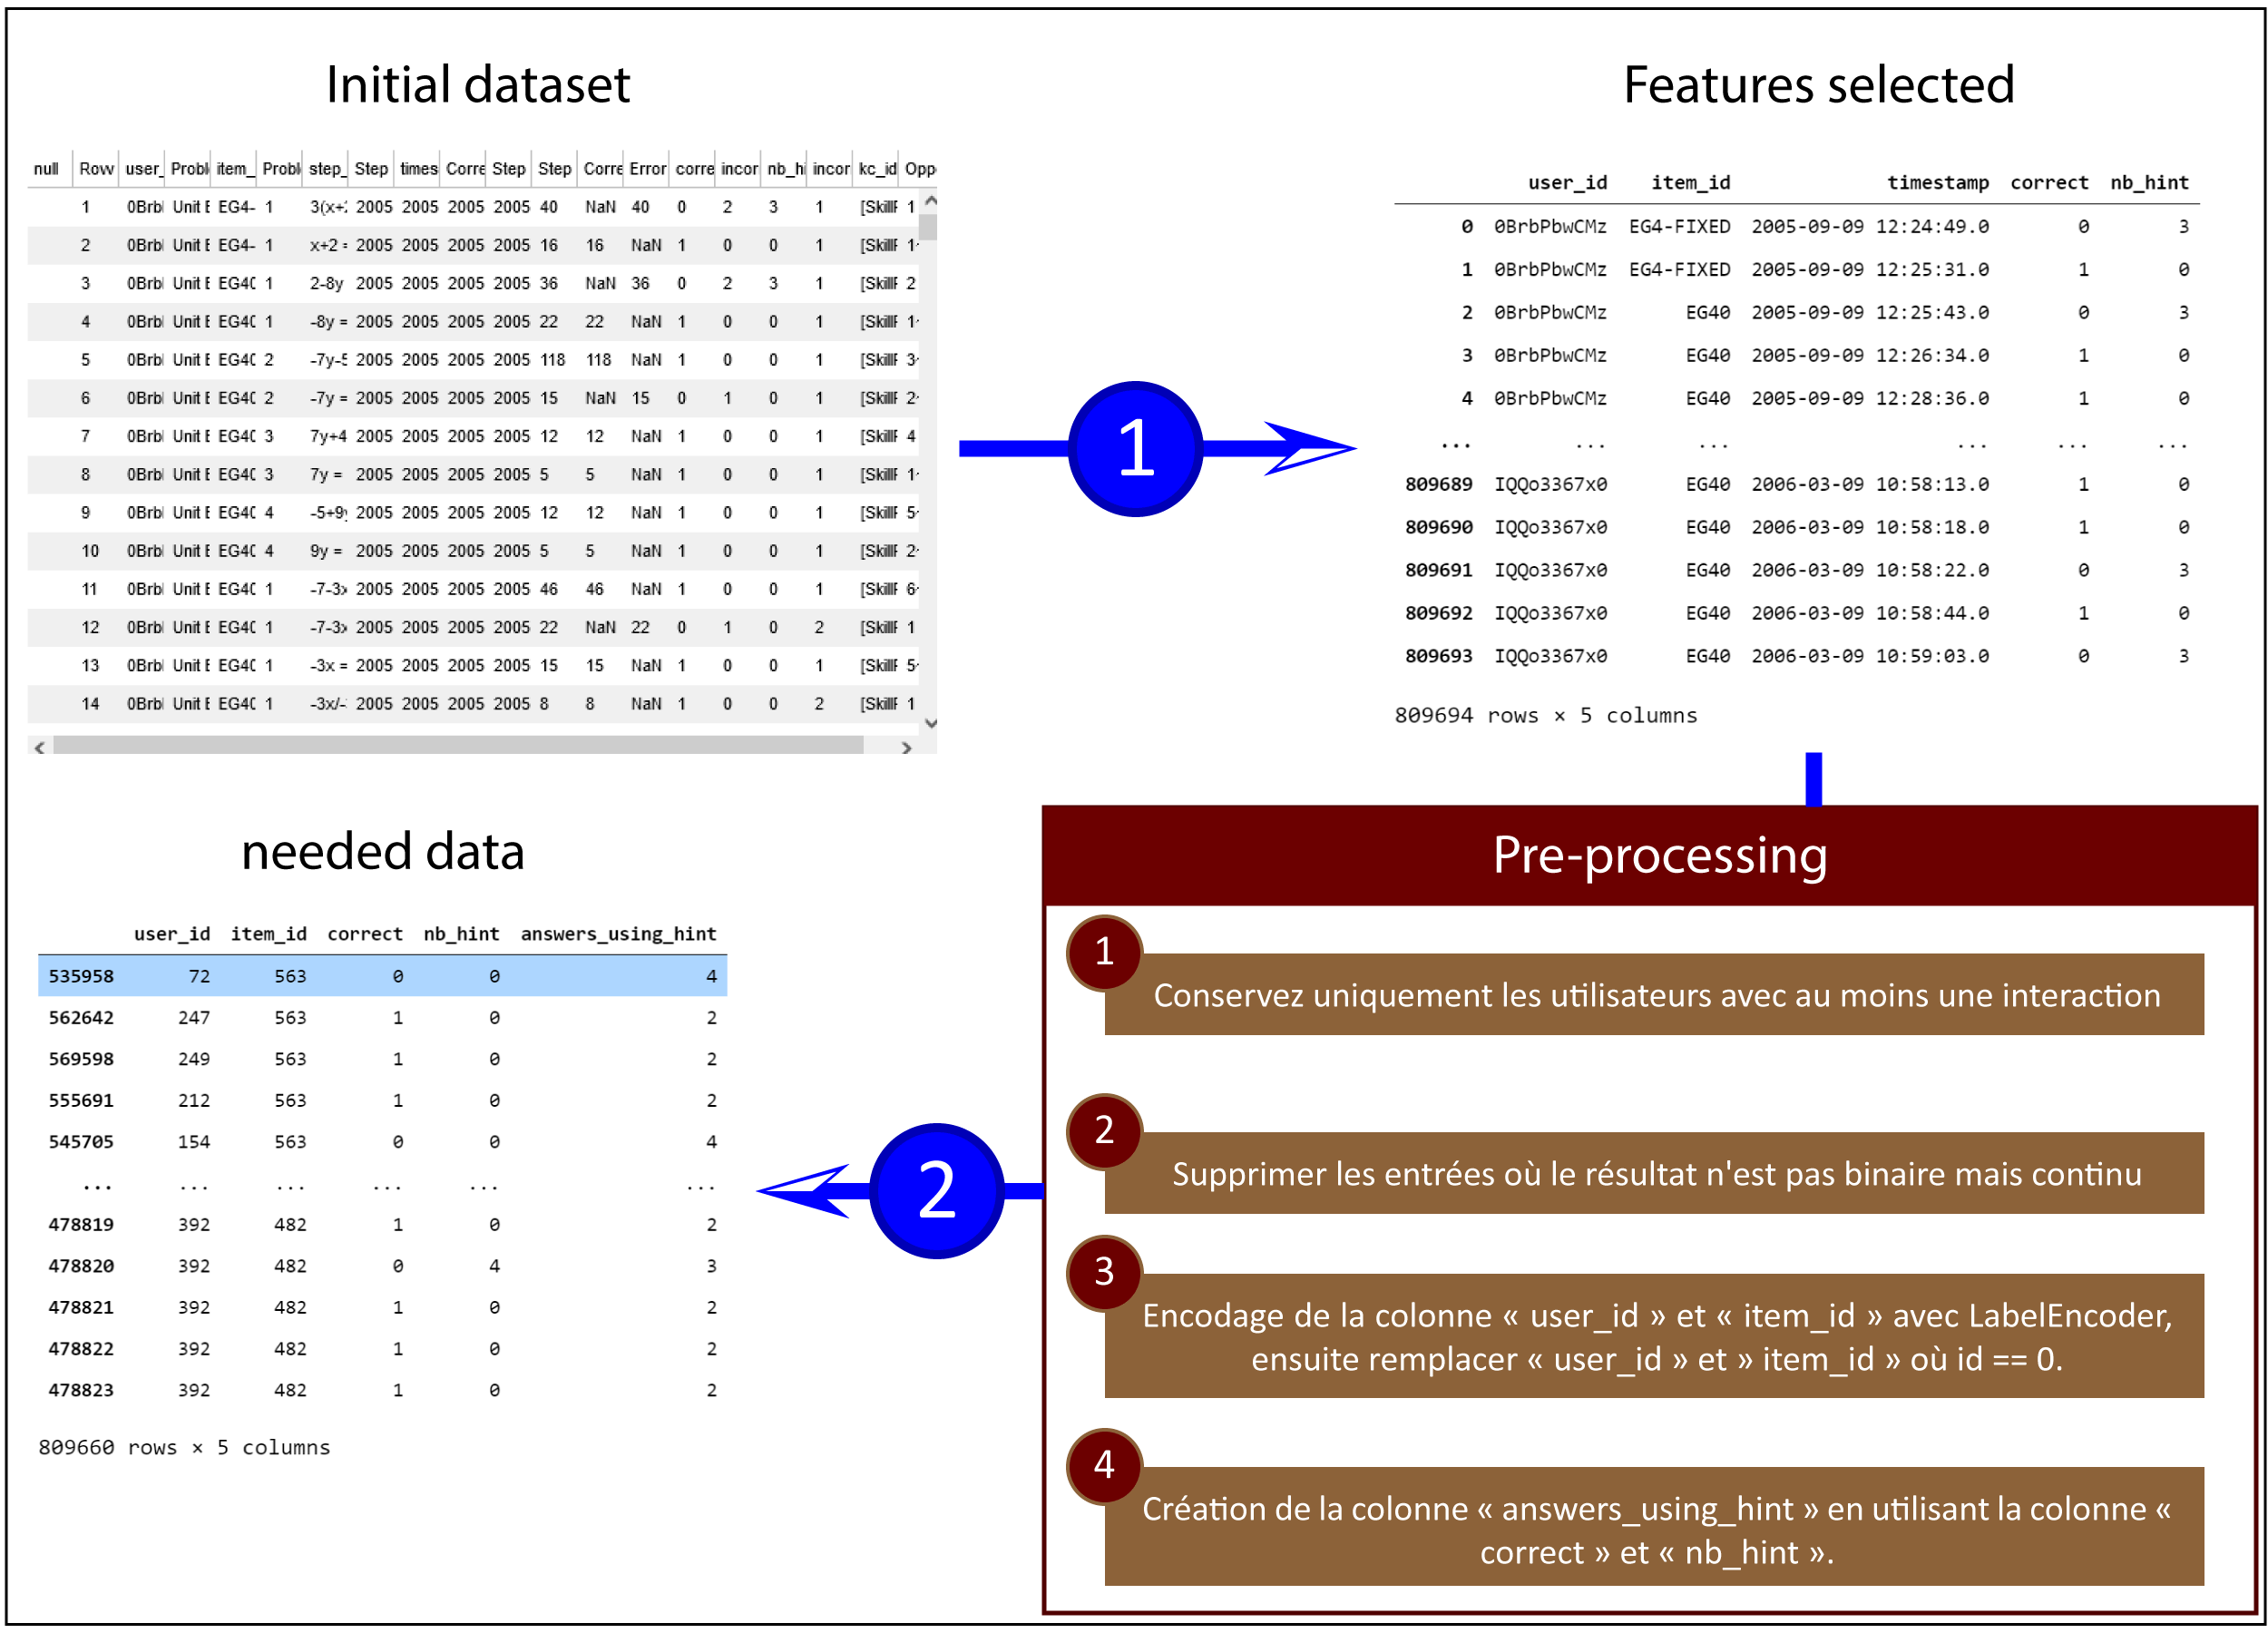
\includegraphics[width=\textwidth]{images/chapitre7/preprocessing_steps.png}
	\end{center}
	\caption{Le pre-processing du dataset.}
	\label{datatset_pre-processing}
\end{figure}

\begin{description}
    \item[\textbf{Première étape : }] dans notre travail, nous nous concentrons sur la performance de l'apprenant qui est liée à l'item, au résultat obtenu par l'apprenant : (correct/incorrect soit 0 ou 1), ou en prenant un indice (hint).
    \item[\textbf{Deuxième étape : }] seuls les apprenants ayant au moins 10 interactions avec les items ont été sélectionner. Les valeurs qui ne sont pas binaire (0 ou 1) dans la colonne « correct » sont éliminées. Les valeurs de la colonne « user\char`_id »  et « item\char`_id » sont encoder et où « id = 0 » est remplacer par le nombre total des apprenants et des items respectivement. L’encodage permet d’encoder les identifiants en valeur numérique, parce que le modèle IRT prend seulement des valeurs numériques à partir de 1. La colonne « answers\char`_using\char`_hint » ajouter au dataset sera utilisé pour calculer la matrice de similarité entre items selon notre critère : réponse correcte avec aide (hints) et sans aide, et incorrecte avec aide et sans aide.Le script python avec lequel la colonne « answers\char`_using\char`_hint » est dans \ref{answersusinghint}.
\end{description}

\newpage
\begin{lstlisting}[language=Python,label={answersusinghint}, 
	morekeywords={self},
	keywordstyle=\ttb\color{deepblue},
	emph={MyClass,__init__},
	emphstyle=\ttb\color{deepred},
	stringstyle=\color{deepgreen},basicstyle=\scriptsize, frame=l,framesep=4.5mm,framexleftmargin=2.5mm,tabsize=2,numbers=left,fillcolor=\color{blueforest!70},rulecolor=\color{blueforest},numberstyle=\normalfont\tiny\color{white}]
	conditions = [
		(needed['correct'] == 1) & (needed['nb_hint'] > 0),
		(needed['correct'] == 1) & (needed['nb_hint'] == 0),
		(needed['correct'] == 0) & (needed['nb_hint'] > 0),
		(needed['correct'] == 0) & (needed['nb_hint'] == 0)
		]
	# 1 ==> Correct avec hint
	# 2 ==> Correct sans hint
	# 3 ==> Incorrect avec hint
	# 4 ==> Incorrect sans hint
	values = [1, 2, 3, 4]
	
	# create a new column and use np.select to assign values to it using our lists as arguments
	needed['answers_using_hint'] = np.select(conditions, values)
\end{lstlisting}

\subsection{Modèle IRT pour une inférence bayésienne}

\subsubsection{Spécification et chargement du modèle}
Nous avons utilisé le modèle de Rasch pour faire l’ajustement bayésien avec Stan en utilisant le script en Stan définit dans le chapitre \ref{chap:irt}. Le script complet est :
\begin{lstlisting}[language=Stan,basicstyle=\scriptsize, frame=l,framesep=4.5mm,framexleftmargin=2.5mm,tabsize=2,numbers=left,fillcolor=\color{blueforest!70},rulecolor=\color{blueforest},numberstyle=\normalfont\tiny\color{white}]
_1pl_model = """
data {
	// numbers of things
	int<lower=1> N;  // number of observations
	int<lower=1> I;  // items,  number of questions  
	int<lower=1> S;  // subjects,  number of users 
	// data
	int<lower=1,upper=I> item[N];
	int<lower=1,upper=S> subject[N];
	int<lower=0,upper=1> grade[N];
}
parameters {
	// parameters
	real ability[S];             //  alpha: ability of student
	real difficulty[I];          //  beta: difficulty of question
	real delta;                   // mean student ability
}
model {
	ability ~ std_normal();         
	difficulty ~ std_normal();   
	delta ~ normal(0.75,1);
	for(n in 1:N)
		grade[n] ~ bernoulli_logit(ability[subject[n]] - difficulty[item[n]] + delta);
}
"""
\end{lstlisting}
Nous n’avons pas utilisé le bloc « generated quantities » parce qu’en ajoutant ce bloc la taille de modèle ajusté devient déraisonnablement grande. Avant de charger et compiler le modèle, Stan prend les données dans un dictionnaire, où les noms des clés doivent être identiques aux noms spécifiés dans la section data du modèle. Les données de notre dataset dans format dictionnaire est :

\begin{lstlisting}[language=Python,basicstyle=\scriptsize, frame=l,framesep=4.5mm,framexleftmargin=2.5mm,tabsize=2,numbers=left,fillcolor=\color{blueforest!70},rulecolor=\color{blueforest},numberstyle=\normalfont\tiny\color{white}]
	{'I': 1084,
	'N': 809660,
	'S': 569,
	'grade': array([0, 1, 1, ..., 1, 1, 1]),
	'item': array([563, 563, 563, ..., 482, 482, 482]),
	'subject': array([ 72, 247, 249, ..., 392, 392, 392])}
\end{lstlisting}

\subsubsection{Compilation du modèle et échantillonnage }

Après avoir spécifier le modèle, la compilation (en code c++) est faite en utilisant la fonction \colorbox{gray!30}{stan.build()} qui prend en paramètre le modèle , les données et random\char`_seed qui contrôle l’effet aléatoire. Le script est :
\begin{lstlisting}[language=Stan,basicstyle=\normalsize, frame=l,framesep=4.5mm,framexleftmargin=2.5mm,tabsize=2,numbers=left,fillcolor=\color{blueforest!70},rulecolor=\color{blueforest},numberstyle=\normalsize\tiny\color{white}]
	posteriori = stan.build(_1pl_model,data=train_data,random_seed=2021)
\end{lstlisting}

Une fois le modèle compiler avec les données, la méthode \colorbox{gray!30}{sample()} fait des échantillonnages dans les distributions spécifier dans le modèle. La méthode \colorbox{gray!30}{sample()} prend en paramètre \colorbox{gray!30}{num\char`_chains}   le nombre de chaine  qui sont exécuter en parallèle, \colorbox{gray!30}{num\char`_samples}  le nombre d’échantillon à générer, \colorbox{gray!30}{num\char`_warmup}  le nombre d’échantillon initial à rejeter qui sont généralement loin d'être optimales et \colorbox{gray!30}{num\char`_thin} spécifie un intervalle d'échantillonnage auquel les échantillons sont conservés.

\begin{lstlisting}[language=Stan,basicstyle=\normalsize, frame=l,framesep=4.5mm,framexleftmargin=2.5mm,tabsize=2,numbers=left,fillcolor=\color{blueforest!70},rulecolor=\color{blueforest},numberstyle=\normalsize\tiny\color{white}]
	fit = posteriori.sample(num_chains=2, num_samples=50000,
	      num_warmup=1000,num_thin=1)
\end{lstlisting}



\subsubsection{Résultats d’échantillonnage, diagnostique du modèle, prédiction et validation}


Une fois l’échantillonnage terminé, l’objet \colorbox{gray!30}{stanfit} renvoyer par la méthode \colorbox{gray!30}{sample()} contient la sortie dérivée de l’ajustement du modèle c’est-à dire les résultats de l’inférence. L’objet \colorbox{gray!30}{fit} du modèle est afficher dans le tableau de la figure \ref{stanfit_object}. La figure \ref{model_trace-plot} affiche les distributions postérieures des paramètres du modèle pour toute les itérations et la figure \ref{params_posterior_distribution} la moyenne des distributions postérieures.
\begin{figure}[H]
	\begin{center}
		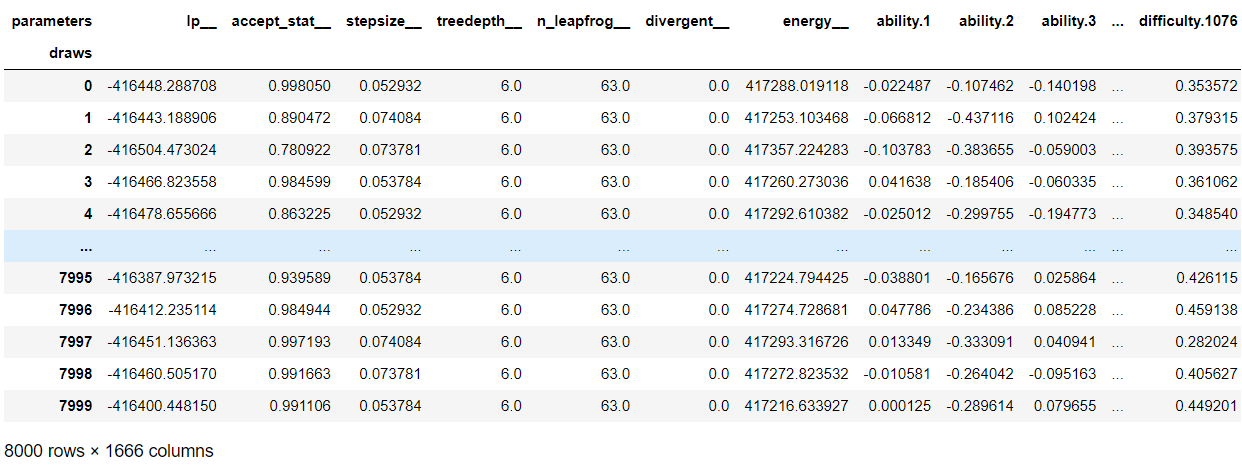
\includegraphics[width=\textwidth]{images/chapitre7/stanfit_object.png}
	\end{center}
	\caption{L’objet stanfit de notre modèle.}
	\label{stanfit_object}
\end{figure}


\begin{figure}[H]
	\begin{center}
		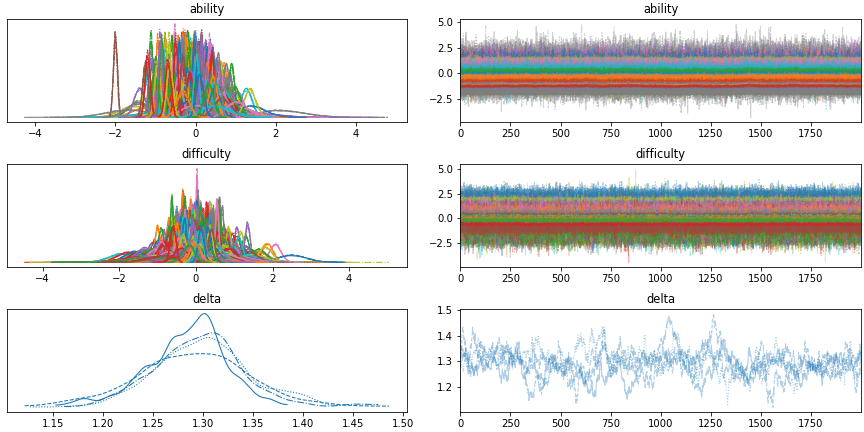
\includegraphics[width=\textwidth]{images/chapitre7/model_plot-trace.png}
	\end{center}
	\caption{Les distributions postérieures du modèle.}
	\label{model_trace-plot}
\end{figure}

\begin{figure}[H]
	\begin{center}
		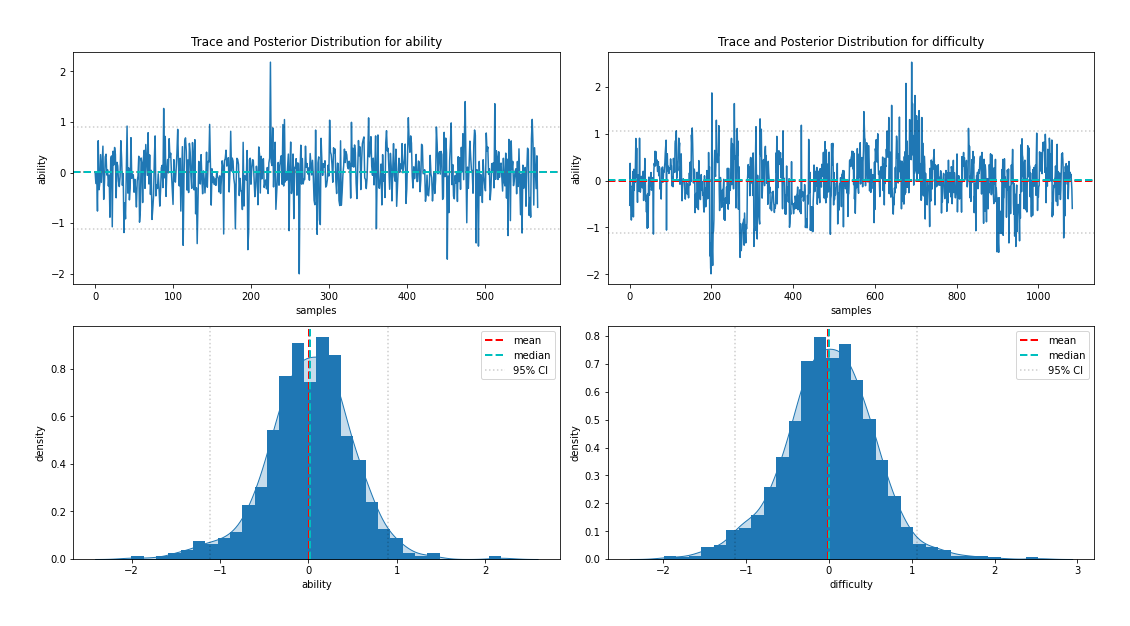
\includegraphics[width=\textwidth]{images/chapitre7/params_posterior_distribution.png}
	\end{center}
	\caption{La moyenne des distributions postérieures du modèle.}
	\label{params_posterior_distribution}
\end{figure}

En plus des valeurs des paramètres du modèle, le tableau de la figure contient également d’autre valeurs des paramètres utilisés par l'échantillonneur qui vont servir de diagnostique.
L'étiquette \colorbox{gray!30}{lp\char`_\char`_} est pour les densités logarithmiques (jusqu'à une constante additive), \colorbox{gray!30}{accept\char`_stat\char`_\char`_} est pour les probabilités d'acceptation, \colorbox{gray!30}{stepsize\char`_\char`_} est pour la taille de pas de l'intégrateur leapfrog pour simuler l'hamiltonien, \colorbox{gray!30}{treedepth\char`_\char`_} est la profondeur de l'arbre exploré par l'échantillonneur sans demi-tour (Journal base 2 du nombre d'évaluations de densité et de gradient log), \colorbox{gray!30}{n\char`_leapfrog\char`_\char`_} est le nombre d'évaluations de densité et de gradient, \colorbox{gray!30}{divergent\char`_\char`_} est un indicateur indiquant une instabilité numérique lors de l'intégration numérique entraînant la non conservation de l'hamiltonien, et \colorbox{gray!30}{energy\char`_\char`_} est la valeur hamiltonienne. \\

\textbf{Le BFMI :} Bayesian Fraction of Missing Information, bfmi inférieur à 0,2 indique qu’il faut peut-être reparamétrer votre modèle.

\begin{figure}[H]
	\begin{center}
		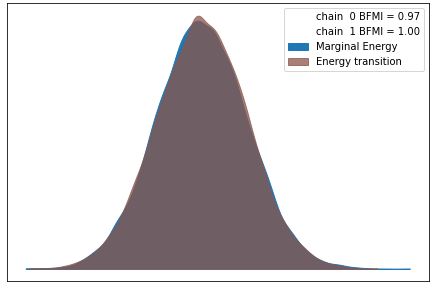
\includegraphics[scale=0.5]{images/chapitre7/model_energy.png}
	\end{center}
	\caption{BFMI du modèle.}
	\label{bfmi_of_model}
\end{figure}

\textbf{Le Rhat :} un Rhat > 1.1 indique généralement des problèmes d'ajustement et si Rhat est d'environ 1, alors il n’y aura aucune diminution de la variance d'échantillonnage, quelle que soit la durée d’itération, et donc la chaîne de Markov est susceptible (mais pas garantie) d'avoir convergé. Celui ne notre modèle est d'environ 1 pour tous les paramètres.

\begin{figure}[H]
	\begin{center}
		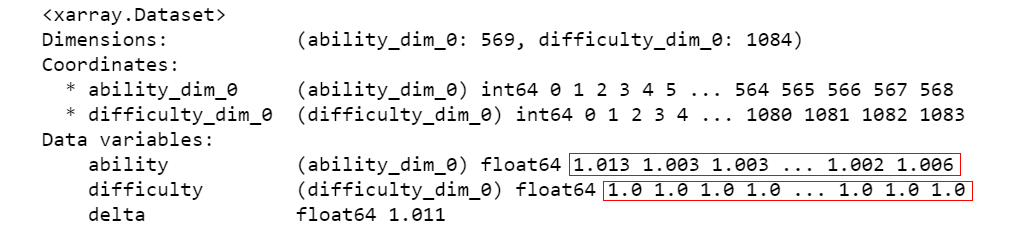
\includegraphics[width=\textwidth]{images/chapitre7/output_of_rhat.png}
	\end{center}
	\caption{Le Rhat du modèle.}
	\label{output_of_rhat}
\end{figure}
\textbf{Vérification des divergences }: aucune divergence dans le modèle comme le montre la figure \ref{diverging_output}.

\begin{figure}[H]
	\begin{center}
		\includegraphics[width=\textwidth]{images/chapitre7/diverging_output.png}
	\end{center}
	\caption{La sortie de la divergence du modèle.}
	\label{diverging_output}
\end{figure}

Ensuite après diagnostique du modèle, les valeurs des paramètres obtenu peuvent être utilisé pour faire des prédictions postérieures en utilisant la fonction logistique de Rasch \ref{posterior_probability_distribution} ou bien faire des prédictions directement en utilisant le bloc generated quantities \ref{generated_quantities} et aussi récupérer le log de vraisemblance (log likelihood) qui est utilisé pour comparer plusieurs modèles (sélection de modèle). Mais l’utilisation de ce bloc entraine un coût de calcul et d'utilisation de la mémoire. Le script est utilisé pour prédire la probabilité de réussite à un item \ref{pred_script}. C’est ainsi que l’ajustement bayésien des réponses aux items a été fait avec un modèle d’inférence bayésien.

\begin{lstlisting}[language=Python,label={pred_script},stringstyle=\color{deepgreen},basicstyle=\scriptsize, frame=l,framesep=4.5mm,framexleftmargin=2.5mm,tabsize=2,numbers=left,fillcolor=\color{blueforest!70},rulecolor=\color{blueforest},numberstyle=\normalfont\tiny\color{white}]
ability = np.mean(fit['ability'],axis=1)
difficulty = np.mean(fit['difficulty'],axis=1)
y_pred = []
for i in range(0,len(needed)):
	diff = train_data['item'][i] # Item index
	abilt = train_data['subject'][i] # Subject index
	p = np.exp(ability[abilt - 1 ] - difficulty[diff - 1])/(1+np.exp(ability[abilt - 1] 
	   - difficulty[diff - 1]))
	y_pred.append(p)
y_pred = np.round(y_pred).astype(int)
\end{lstlisting}

Nous terminons donc cette étape avec la validation des prédictions faite par le script. Plusieurs métriques peuvent être utilisé pour valider les prédictions d’un modèle de classification parce qu’on a deux classes (réponses correcte ou incorrecte).

\begin{itemize}
	\item \textbf{Accuracy :}
	\item \textbf{Mean squared error :}
	\item \textbf{Roc auc score :}
	\item \textbf{Cohen kappa :}	
\end{itemize}
Celui du modèle sont afficher dans le tableau et roc\char`_auc\char`_score est illustré par la figure.

\begin{minipage}{\textwidth}
	\begin{minipage}[b]{0.49\textwidth}
	\centering
	\includegraphics[width=\textwidth]{images/chapitre7/roc_auc.png}
	\captionof{figure}{A table beside a figure}
\end{minipage}
\hfill
\begin{minipage}[b]{0.49\textwidth}
	\centering
	\begin{tabular}{|m{3cm}|m{3cm}|}
	\hline
	\rowcolor{blueforest}
	\color{white} \textbf{Métriques} & \color{white} \textbf{valeurs}  \\
	\hline\hline
	mse & 0.421189 \\ \hline
	kappa & 0.1587 \\ \hline
	auc & 0.611 \\ \hline
	acc & 0.57881 \\ \hline
	\end{tabular}
	\captionof{table}{A table beside a figure}
	\end{minipage}
\end{minipage}

\subsection{Clustering hard et soft de la matrice de similarité}

\subsubsection{Création de la matrice de similarité}
Les données collecter dans la partie [\ref{collect_encoding}] et ceux de l’ajustement bayésien avec le modèle de Rasch (c’est-à dire les prédictions faites faire le modèle d’inférence bayésien) sont utilisée pour créer la matrice de réponse selon quatre catégories : correct avec aide (CH) et sans aide (CS), et incorrect avec aide (IH) et sans aide (IS). La matrice de réponses est ensuite utilisée pour créer la matrice de similarité entre items avec le coefficient de kappa. La figure \ref{similarity_steps} illustre toutes les étapes. 

\begin{figure}[H]
	\begin{center}
		\includegraphics[width=\textwidth]{images/chapitre7/similarity_steps.png}
	\end{center}
	\caption{Les étapes de calcule de la matrice de similarité.}
	\label{similarity_steps}
\end{figure}

Le script utiliser pour calculer la matrice des sommes des réponses est :
\begin{lstlisting}[language=Python,basicstyle=\scriptsize, frame=l,framesep=4.5mm,framexleftmargin=2.5mm,tabsize=2,numbers=left,fillcolor=\color{blueforest!70},rulecolor=\color{blueforest},numberstyle=\normalfont\tiny\color{white}]
	def createSumMatrix(data):
    column_names = data['item_id'].unique()
    rows_name = ["CH","CS","IH","IS"]
    columns = pd.DataFrame(columns = column_names)
    index = pd.DataFrame(rows_name, columns = ['catégories'])
    sumOfAnswers_df = pd.concat([index,columns], axis=1)
    sumOfAnswers_df = sumOfAnswers_df.set_index("catégories")
    sumOfAnswers_df = sumOfAnswers_df.replace(np.nan,0)
    column_name = data['item_id'].unique()
    rows_name = data['user_id'].unique()
    for i in tqdm(rows_name):
        for j in column_name:
            dictVal = data[(data["user_id"] == i) & (data["item_id"] == j)]['answers_using_hint'].value_counts()
            chVal = sumOfAnswers_df.loc["CH",j]
            csVal = sumOfAnswers_df.loc["CS",j]
            ihVal = sumOfAnswers_df.loc["IH",j]
            isVal = sumOfAnswers_df.loc["IS",j]
            if len(dictVal) != 0:
                for key, value in dictVal.items():
                    key = int(key)
                    if key == 1:
                        chVal = int(chVal) + value
                    elif key == 2:
                        csVal = int(csVal) + value
                    elif key == 3:
                        ihVal = int(ihVal) + value
                    elif key == 4:
                        isVal = int(isVal) + value
                sumOfAnswers_df.loc["CH",j] = chVal
                sumOfAnswers_df.loc["CS",j] = csVal
                sumOfAnswers_df.loc["IH",j] = ihVal
                sumOfAnswers_df.loc["IS",j] = isVal
	return sumOfAnswers_df
	
\end{lstlisting}

La matrice de similarité entre items est calculée avec le code \ref{similarity_code}.
\begin{lstlisting}[language=Python,label={similarity_code}, basicstyle=\scriptsize, frame=l,framesep=4.5mm,framexleftmargin=2.5mm,tabsize=2,numbers=left,fillcolor=\color{blueforest!70},rulecolor=\color{blueforest},numberstyle=\normalfont\tiny\color{white}]
	def item_to_item_similarity1(data):
    column_names = data.columns
    columns = pd.DataFrame(columns = column_names)
    items = pd.DataFrame(column_names, columns = ['item_id'])
    items_similarity = pd.concat([items,columns], axis=1)
    items_similarity = items_similarity.set_index("item_id")
    index = data.columns
    for i in tqdm(index):
        for j in index:
            val = cohen_kappa_score(data[i],data[j])
            items_similarity.loc[i,j] = val
    return items_similarity
\end{lstlisting}

\subsubsection{Analyse en composantes principales (ACP)}


\begin{lstlisting}[language=Python,label={pca_code}, basicstyle=\scriptsize, frame=l,framesep=4.5mm,framexleftmargin=2.5mm,tabsize=2,numbers=left,fillcolor=\color{blueforest!70},rulecolor=\color{blueforest},numberstyle=\normalfont\tiny\color{white}]
	pca = decomposition.PCA(n_components=2)
    pca.fit(items_similarity)
    features = pca.transform(items_similarity)
\end{lstlisting}
\subsubsection{Clustering hard}


\subsubsection{Clustering Soft}


\subsubsection{Validation du clustering}



\section{Conclusion}


\addcontentsline{toc}{part}{Conclusion Générale}
\chapter*{Conclusion Générale et Perspectives }
\markboth{\textbf{CONCLUSION G\'EN\'ERALE ET PERSPECTIVES }}{}
\thispagestyle{empty}
\section*{Conclusion Générale}
Dans ce mémoire, nous avons travaillé sur l'intégration des méthodes du data mining dans les systèmes d'apprentissage qui ont pour but d’optimiser les méthodes d'apprentissage, de construire et d’évaluer des échelles de mesure, de gérer un grand nombre d’item, ainsi que les techniques de regroupement des items en composants de connaissances. \\
Les paramètres estimés à l’aide de l’inférence bayésienne pour les modèles de la théorie de la réponse aux items peuvent être utilisé pour évaluer la qualité des échelles de mesures et de prédire les scores des apprenants avant d’effectuer la collecte de données pour faire un regroupement des items selon leurs similitudes. \\
Dans ce travail, nous avons eu deux contributions \\
Dans la première contribution, nous avons proposé une étape d’analyse et de validation des données des systèmes éducatif à l’aide de l’inférence bayésienne et des modèles de la théorie de la réponse aux items. Cette étape a été utilisé comme un workflow bayésien, c’est-à-dire un processus itératif jusqu’à l’obtention d’un modèle acceptable ou provisoirement acceptable. Les paramètres des modèles IRT ainsi obtenu décrive les compétences des apprenants sur un continuum de trait latent d’une part et d’autre part les propriétés de l’item notamment, sa difficulté, son pouvoir de discrimination, le rôle que la "chance" (réponses "au hasard") peut jouer dans certains cas. Une fois l’obtention d’un modèle acceptable ou provisoirement acceptable, les valeurs de ces paramètres peuvent être utilise pour prédire la probabilité qu’un apprenant obtient une réponse correcte. Enfin les valeurs des métriques entre les données observées et ceux prédit par les modèles peuvent être utilisé pour comparer les modèles IRT avec des spécifications alternatives, ou pour éclairer une décision sur l'intérêt de collecter ce type de données. \\
Dans la deuxième contribution, un regroupement des items en composante de connaissance a été appliquer avec une méthode de clustering partitionel (à l'aide de l'algorithme K-means), hiérarchique (à l'aide de l'algorithme hiérarchique agglomérative) et floue (à l'aide de l'algorithme c-means). Ces méthodes de clustering ont utilisé la matrice de similarité Item-Item calculer à partir du nombre correct et incorrect des réponses avec aide et sans aide, et le coefficient de kappa pour le calcul de degré de similarité. \\

\section*{\textbf{Perspectives}}
A la fin de ce projet de fin d’études, nous avons dégagé les perspectives suivantes à développer dans l’avenir pour une amélioration de ce travail :

\begin{itemize}
    \item Extension des modèles IRT mentionnés dans ce mémoire aux modèles à plusieurs niveaux de sorte qu'ils prennent en compte les variations de capacités entre les unités de groupe telles que les écoles, ainsi qu'au sein des unités de groupe. Ces modèles à plusieurs niveaux distingueront ainsi les capacités au niveau individuel(étudiants), au niveau du groupe (classes), ou les deux.
    \item Estimations des probabilités de réussite a un item avec l’algorithme Bayesian Knowledge Tracing (BKT).
    \item Appliquer d’autre coefficient de similarité comme Yule, Fisher, Sokal et aussi le critère de calcule de similitude entre items.
\end{itemize}




%%%%%%%%%%%%%% Appendix  %%%%%%%%%
%\thirdpart
\clearpage
\appendix
\addcontentsline{toc}{part}{Annexe}
%\markboth{\textbf{Annexe}}{}
\thispagestyle{empty}
\chapter{Les modèles IRT en code Stan.}


\begin{lstlisting}[language=Stan,caption={Code Stan pour le modèle de Rasch},basicstyle=\scriptsize, frame=lines,framesep=4.5mm,framexleftmargin=2.5mm,tabsize=2,numbers=left,fillcolor=\color{white},rulecolor=\color{black},numberstyle=\normalfont\scriptsize\color{black}]
    _1pl_model = """
    data {
        // numbers of things
        int<lower=1> N;  // number of observations
        int<lower=1> I;  // items,  number of questions  
        int<lower=1> S;  // subjects,  number of users 
        // data
        int<lower=1,upper=I> item[N];
        int<lower=1,upper=S> subject[N];
        int<lower=0,upper=1> grade[N];
        // data for posterior prediction using new data also used for Cross-validation
        int<lower=1> N_new;
        int<lower=1,upper=I> item_new[N_new];
        int<lower=1,upper=S> subject_new[N_new];
    }
    parameters {
        // parameters
        real ability[S];             //  alpha: ability of student
        real difficulty[I];          //  beta: difficulty of question
        real delta;                   // mean student ability
    }
    model {
        ability ~ normal(0,1);         
        difficulty ~ normal(0,1);   
        delta ~ normal(0.75,1);
        for(n in 1:N)
            grade[n] ~ bernoulli_logit(ability[subject[n]] - difficulty[item[n]] + delta);
    }
    generated quantities {
        int<lower=0,upper=1> y_pred[N];
        int<lower=0,upper=1> yNew_pred[N_new];
        vector[N] log_lik;

        for(n in 1:N){
            y_pred[n] = bernoulli_logit_rng(ability[subject[n]] - difficulty[item[n]] + delta);
            log_lik[n] = bernoulli_logit_lpmf( grade[n] | ability[subject[n]] - difficulty[item[n]]
            + delta);
        }
        for (n in 1:N_new) {
            yNew_pred[n] = bernoulli_logit_rng(ability[subject_new[n]] - difficulty[item_new[n]] + delta);                                             
        }
    }
    """
\end{lstlisting}
\newpage

\begin{lstlisting}[language=Stan,caption={Code Stan pour 2PL},basicstyle=\scriptsize, frame=lines,framesep=4.5mm,framexleftmargin=2.5mm,tabsize=2,numbers=left,fillcolor=\color{white},rulecolor=\color{black},numberstyle=\normalfont\scriptsize\color{black}]
    _2pl_model = """
    data {
        // numbers of things
        int<lower=1> N;  // number of observations
        int<lower=1> I;  // items,  number of questions  
        int<lower=1> S;  // subjects,  number of users 
        // data
        int<lower=1,upper=I> item[N];
        int<lower=1,upper=S> subject[N];
        int<lower=0,upper=1> grade[N];
        // data for posterior prediction using new data also used for Cross-validation
        int<lower=1> N_new;
        int<lower=1,upper=I> item_new[N_new];
        int<lower=1,upper=S> subject_new[N_new];
    }
    parameters {
        // parameters
        real ability[S];             //  alpha: ability of student
        real difficulty[I];          //  beta: difficulty of question
        vector<lower=0>[I] discrimination;      // discrimination of question
        real delta;                   // mean student ability
    }
    model {
        ability ~ normal(0,1);         
        difficulty ~ normal(0,1);   
        discrimination ~ lognormal(0,1);
        delta ~ normal(0.75,1);
        grade ~ bernoulli_logit(discrimination[item] .* (ability[subject] - (difficulty[item] + delta)));	
    }
    generated quantities {
        int<lower=0,upper=1> y_pred[N];
        int<lower=0,upper=1> yNew_pred[N_new];
        vector[N] log_lik;

        for(n in 1:N){
            y_pred[n] = bernoulli_logit_rng(discrimination[item[n]] * (ability[subject[n]] - (difficulty[item[n]] + delta)));
            log_lik[n] = bernoulli_logit_lpmf( grade[n] | discrimination[item[n]] * (ability[subject[n]] - (difficulty[item[n]] + delta)));
        }
        for (n in 1:N_new) {
            yNew_pred[n] = bernoulli_logit_rng(discrimination[item[n]] * (ability[subject_new[n]] - (difficulty[item_new[n]] + delta)));                             
        }
    }
    """
\end{lstlisting}

\newpage

\begin{lstlisting}[language=Stan,caption={Code Stan pour 3PL},basicstyle=\scriptsize, frame=lines,framesep=4.5mm,framexleftmargin=2.5mm,tabsize=2,numbers=left,fillcolor=\color{white},rulecolor=\color{black},numberstyle=\normalfont\scriptsize\color{black}]
    _3pl_model = """
    data {
        // numbers of things
        int<lower=1> N;  // number of observations
        int<lower=1> I;  // items,  number of questions  
        int<lower=1> S;  // subjects,  number of users 
        // data
        int<lower=1,upper=I> item[N];
        int<lower=1,upper=S> subject[N];
        int<lower=0,upper=1> grade[N];
        // data for posterior prediction using new data also used for Cross-validation
        int<lower=1> N_new;
        int<lower=1,upper=I> item_new[N_new];
        int<lower=1,upper=S> subject_new[N_new];
    }
    parameters {
        // parameters
        real ability[S];             //  alpha: ability of student
        real difficulty[I];          //  beta: difficulty of question
        vector<lower=0>[I] discrimination;      // discrimination of question
        vector<lower=0,upper=1>[I] guessing;    
        real delta;                   // mean student ability
    }
    model {
        ability ~ normal(0,1);         
        difficulty ~ normal(0,1);   
        discrimination ~ lognormal(0,1);
        guessing ~ beta(5,17);
        delta ~ normal(0.75,1);
        grade ~ bernoulli(guessing[item] + ((1-guessing[item]).*(inv_logit(discrimination[item] .* (ability[subject] - (difficulty[item] + delta))))));
    }
    generated quantities {
        int<lower=0,upper=1> y_pred[N];
        int<lower=0,upper=1> yNew_pred[N_new];
        vector[N] log_lik;

        for(n in 1:N){
            y_pred[n] = bernoulli_rng(guessing[item[n]] + ((1-guessing[item[n]]) * (inv_logit(discrimination[item[n]] .* (ability[subject[n]] - (difficulty[item[n]] + delta))))));
            log_lik[n] = bernoulli_lpmf( grade[n] | guessing[item[n]] + ((1-guessing[item[n]]) * (inv_logit(discrimination[item[n]] .* (ability[subject[n]] - (difficulty[item[n]] + delta))))));
        }
        for (n in 1:N_new) {
            yNew_pred[n] = bernoulli_rng(guessing[item[n]] + ((1-guessing[item[n]]) * (inv_logit(discrimination[item[n]] .* (ability[subject[n]] - (difficulty[item[n]] + delta))))));                                             
        }
    }
    """
\end{lstlisting}

\begin{lstlisting}[language=Stan,caption={Code Stan pour le modèle de Rasch avec cross-validation},basicstyle=\scriptsize, frame=lines,framesep=4.5mm,framexleftmargin=2.5mm,tabsize=2,numbers=left,fillcolor=\color{white},rulecolor=\color{black},numberstyle=\normalfont\scriptsize\color{black}]
    _1pl_cross_val_model = """
    functions {
        int[] permutation_rng(int N) {
            int y[N];
            for (n in 1:N)
                y[n] = n;
            vector[N] theta = rep_vector(1.0 / N, N);
            for (n in 1:N){
                int i = categorical_rng(theta);
                int temp = y[n];
                y[n] = y[i];
                y[i] = temp;
            }
            return y;
        }
    }
    
    data {
      // numbers of things
      
      int<lower=1> N;  // number of observations
      int<lower = 0, upper = N> N_test;
      int<lower=1> I;  // items,  number of questions  
      int<lower=1> S;  // subjects,  number of users
      
      // data
      
      int<lower=1,upper=I> item[N];
      int<lower=1,upper=S> subject[N];
      int<lower=0,upper=1> grade[N];
    }
    transformed data {
      int N_train = N - N_test;
      int permutation[N] = permutation_rng(N);
      // train
      int item_train[N_train] = item[permutation[1 : N_train]];
      int subject_train[N_train]  = subject[permutation[1 : N_train]];
      int grade_train[N_train]  = grade[permutation[1 : N_train]];
      int s_train = size(subject_train);
      int i_train = size(item_train);
      
      
      // test
      int item_test[N_test] = item[permutation[N_train + 1 : N]];
      int subject_test[N_test] = subject[permutation[N_train + 1 : N]];
      int grade_test[N_test] = grade[permutation[N_train + 1 : N]];
    }
    parameters {
      // parameters
      real ability[s_train];             //  alpha: ability od student
      real difficulty[i_train];          //  beta: difficulty of question
      real delta;                   // man student ability
      
    }
    model {
    
      ability ~ normal(0,1);         
      difficulty ~ normal(0,1);   
      delta ~ normal(0.75,1);
      
      for (n in 1:N_train) {
          grade_train[n] ~ bernoulli_logit(ability[subject_train[n]] - difficulty[item_train[n]] + delta);
      }
      
    }
    generated quantities {
      int<lower=0,upper=1> grade_pred[N_test];
      int<lower=0,upper=1> grade_observed[N_test];
      grade_observed = grade_test;
      
      for (n in 1:N_test) {
        grade_pred[n] = bernoulli_logit_rng(ability[subject_test[n]] - difficulty[item_test[n]] + delta);
      }
    }
    """
\end{lstlisting}

\chapter{Les distributions des modèles.}
\begin{figure}[H]
	\begin{center}
		\includegraphics[width=\textwidth]{images/annexe/model_plot-trace2.png}
	\end{center}
	\caption{Les distributions postérieures du modèle logistique à deux paramètres.}
	\label{model_trace-plot2}
\end{figure}

\begin{figure}[H]
	\begin{center}
		\includegraphics[width=\textwidth]{images/annexe/params_posterior_distribution2.png}
	\end{center}
	\caption{Distribution postérieure de la capacité de l’apprenant[72], de la difficulté de l’item[563] et de la discrimination de l’item[563] du modèle 2PL.}
	\label{params_posterior_distribution_2pl}
\end{figure}

\begin{figure}[H]
	\begin{center}
		\includegraphics[width=\textwidth]{images/annexe/model_plot-trace3.png}
	\end{center}
	\caption{Les distributions postérieures du modèle logistique à trois paramètres.}
	\label{model_trace-plot3}
\end{figure}

\begin{figure}[H]
	\begin{center}
		\includegraphics[width=\textwidth]{images/annexe/params_posterior_distribution3.png}
	\end{center}
	\caption{Distribution postérieure de la capacité de l’apprenant[72], de la difficulté de l’item[563], de la discrimination de l’item[563] et de la chance de deviner la reponse correcte de l'item[563] du modèle 2PL.}
	\label{params_posterior_distribution_3pl}
\end{figure}
%%%%%%%%%% REFERENCES BIBLIOGRAPHIQUES %%%%%%%%%
\clearpage	
%\addcontentsline{toc}{part}{}
%\addtocontents{toc}{\protect\setcounter{tocdepth}{0}}
%\thispagestyle{empty}
\addtocontents{toc}{\bigskip}% perhaps as well
\begin{singlespace}
\bibliographystyle{ieeetr}
%\markboth{Bibliographie}{}
\bibliography{biblo}
\end{singlespace}
\end{document}